\documentclass[11pt]{article}

% --- Packages ---
\usepackage[usenames, dvipsnames]{color} % Cool colors
\usepackage{enumerate, amsmath, amsthm, amssymb, mathrsfs, algorithm, algpseudocode, fontawesome, pifont, subfig, fullpage, csquotes, dashrule, tikz, bbm, booktabs, bm, hyperref, wasysym}
\usepackage[framemethod=TikZ]{mdframed}
\usepackage[numbers]{natbib}
\usepackage[normalem]{ulem}

% --- Misc. ---
\hbadness=10000 % No "underfull hbox" messages.
\setlength{\parindent}{0pt} % Removes all indentation.

% -- Commands --
% Dynamically sized mid bar.
\newcommand{\bigmid}{\mathrel{\Big|}}

% ---- Colors and Notes ----
% ---- Colors and Notes ----
\definecolor{dblue}{RGB}{98, 140, 190}
\definecolor{dmblue}{RGB}{169, 193, 219}
\definecolor{dlblue}{RGB}{216, 235, 255}
\definecolor{dred}{RGB}{195, 112, 113}
\definecolor{dorange}{RGB}{230, 169, 132}
\definecolor{dgreen}{RGB}{118, 167, 125}
\definecolor{dlgreen}{RGB}{154, 195, 157}
\definecolor{dtan}{RGB}{221, 215, 200}
\definecolor{dpink}{RGB}{207, 166, 208}
\definecolor{dyellow}{RGB}{255, 248, 199}
\definecolor{dgray}{RGB}{46, 49, 49}

% Lights
\definecolor{dlblue}{RGB}{169, 193, 219}
\definecolor{dlgreen}{RGB}{154, 195, 157}
\definecolor{dyellow}{RGB}{246, 240, 223}


% URL
\newcommand{\durl}[1]{\textcolor{dblue}{\underline{\url{#1}}}}
\newcommand{\tx}[1]{\text{#1}}

% Circled Numbers
\newcommand*\circled[1]{\tikz[baseline=(char.base)]{\node[shape=circle,draw,inner sep=0.7pt] (char) {\footnotesize{#1}};}}
% From: http://tex.stackexchange.com/questions/7032/good-way-to-make-textcircled-numbers

% Under set numbered subset of equation
\newcommand{\numeq}[3]{\underset{\textcolor{#2}{\circled{#1}}}{\textcolor{#2}{#3}}}

\newcommand{\dnote}[1]{\textcolor{dblue}{Dave: #1}}

% ---- Abbreviations -----
\newcommand{\tc}[2]{\textcolor{#1}{#2}}
\newcommand{\ubr}[1]{\underbrace{#1}}
\newcommand{\uset}[2]{\underset{#1}{#2}}
\newcommand{\eps}{\varepsilon}
\newcommand{\KL}[2]{D_{\text{KL}}\left(#1 \mid \mid #2\right)}
\newcommand{\bKL}[2]{D_{\text{KL}}\left(#1 \bigmid \bigmid #2\right)}

% Typical limit:
\newcommand{\nlim}{\underset{n \rightarrow \infty}{\lim}}
\newcommand{\nsum}{\sum_{i = 1}^n}
\newcommand{\nprod}{\prod_{i = 1}^n}

% Add an hrule with some space
\newcommand{\spacerule}{\begin{center}\hdashrule{2cm}{1pt}{1pt}\end{center}}

% Mathcal and Mathbb
\newcommand{\mc}[1]{\mathcal{#1}}
\newcommand{\indic}{\mathbbm{1}}
\newcommand{\bE}{\mathbb{E}}

\newcommand{\longra}{\longrightarrow}
\newcommand{\longla}{\longleftarrow}
\newcommand{\ra}{\rightarrow}
\newcommand{\la}{\leftarrow}

% argmin, argmax.
\DeclareMathOperator*{\argmin}{arg\,min}
\DeclareMathOperator*{\argmax}{arg\,max}

% Quick Matrix.
\newcommand{\mat}[1]{\begin{bmatrix}#1\end{bmatrix}}

% ---- Figures, Boxes, Theorems, Etc. ----

% Basic Image
\newcommand{\img}[2]{
\begin{center}
\includegraphics[scale=#2]{#1}
\end{center}}

% Put a fancy box around things.
\newcommand{\dbox}[1]{
\begin{mdframed}[roundcorner=4pt, backgroundcolor=gray!5]
\vspace{1mm}
{#1}
\end{mdframed}
}

%  --- PROOFS ---

% Inner environment for Proofs
\newmdenv[
  topline=false,
  bottomline=false,
  rightline = false,
  leftmargin=10pt,
  rightmargin=0pt,
  innertopmargin=0pt,
  innerbottommargin=0pt
]{innerproof}

% Proof Command
%\newenvironment{dproof}{\begin{proof} \text{\vspace{2mm}} \begin{innerproof}}{\end{innerproof}\end{proof}\vspace{4mm}}
\newenvironment{dproof}[1][Proof]{\begin{proof}[#1] \text{\vspace{2mm}} \begin{innerproof}}{\end{innerproof}\end{proof}\vspace{4mm}}


% Dave Definition
\newcounter{DaveDefCounter}
\setcounter{DaveDefCounter}{1}

\newcommand{\ddef}[2]
{
\begin{mdframed}[roundcorner=1pt, backgroundcolor=white]
\vspace{1mm}
{\bf Definition \theDaveDefCounter} (#1): {\it #2}
\stepcounter{DaveDefCounter}
\end{mdframed}
}

% Block Quote
\newenvironment{dblockquote}[2]{
\begin{blockquote}
#2
\vspace{-2mm}\hspace{10mm}{#1} \\
\end{blockquote}}

% Algorithm
\newenvironment{dalg}[1]
{\begin{algorithm}\caption{#1}\begin{algorithmic}}
{\end{algorithmic}\end{algorithm}}

% Dave Table
\newenvironment{dtable}[1]
{\begin{figure}[h]
\centering
\begin{tabular}{#1}\toprule}
{\bottomrule
\end{tabular}
\end{figure}}

% For numbering the last of an align*
\newcommand\numberthis{\addtocounter{equation}{1}\tag{\theequation}}


\newtheorem{assumption}{Assumption}
\newtheorem{conjecture}{Conjecture}
\newtheorem{corollary}{Corollary}
\newtheorem{claim}{Claim}
\newtheorem{example}{Example}
\newtheorem{lemma}{Lemma}
\newtheorem{proposition}{Proposition}
\newtheorem{remark}{Remark}
\newtheorem{theorem}{Theorem}


% Nice coloring of references.
\usepackage{hyperref}
\hypersetup{               
    colorlinks=true,              
    breaklinks=true,               
    urlcolor=dblue,
    linkcolor=dgreen,
    linkbordercolor=dgreen,
    citecolor=dblue,
    citebordercolor=dblue
}



\title{ICML 2019 Notes \\ \Large{Long Beach, CA, USA}}
\author{David Abel\footnote{\durl{http://david-abel.github.io}} \\ \durl{david_abel@brown.edu}}
\date{June 2019}

\begin{document}
\maketitle
\tableofcontents
\newpage


This document contains notes I took during the events I managed to make it to at ICML, in Long Beach, CA, USA. Please feel free to distribute it and shoot me an email at \durl{david_abel@brown.edu} if you find any typos or other items that need correcting. 


\section{Conference Highlights}


I spent most of my time at the RL sessions this round (and sadly missed all of the keynotes), so most of my reflections (and notes) are concentrated on RL:
\begin{enumerate}
    \item Lots of great work on off-policy evaluation and off-policy learning (see, for instance, work by \citet{hanna2018importance,le2019batch,fujimoto2018off,gottesman2019combining}, and talks in Section~\ref{sec:off_pol}). These problem settings are really important, as I (and many others) anticipate RL applications will come along with loads of data from sub-optimal policies.
    
    \item Exploration was a hot topic again, and rightfully so (see work by~\citet{mavrin2019distributional,fatemi2019dead,hazan2018provably,shani2019exploration}). Along with off-policy evaluation (and a few others), it's one of the foundational problems in RL that we're in a good position to make serious progress on at the moment.
    
    \item Some really nice work continuing to clarify distributional RL~\cite{bellemare2017distributional} (see work by~\cite{rowland2019statistics,mavrin2019distributional,qu2018nonlinear}).
    
    \item The AI for climate change workshop on Friday was fantastic and extremely well attended (standing room only for the talks I was there for). I've said this after previous conferences, but: as we all know, there are profoundly important problems, and the tools of ML can be extremely effective in their current form.
    
    \item I really think we need to standardize evaluation in RL. Not that we only need a single method for doing so, or a single domain, but at the moment there is far too much variance in evaluation protocols.
    
    \item Loved the panel at the RL for real life workshop (see Section~\ref{sec:panel})
\end{enumerate}



% ------------
% -- Sunday --
% ------------
\newpage
\section{Monday June 10th: Tutorials}
 It begins! Today will be entirely tutorials---I arrived just in time for the second half of the PAC-Bayes tutorial. 

\subsection{Tutorial: PAC-Bayes Theory (Part II)}

The speakers are Benjamin Guedi and John Shawe-Taylor. \\

{\bf Part I Recap:}~\citet{shawe1997pac} carried out PAC~\cite{valiant1984theory} analysis of Bayesian estimators (also see Figure~\ref{fig:pac_bayes}. Shortly after,~\citet{mcallester1999some} presented the first {\it PAC-Bayesian} bound:

\begin{figure}
    \centering
    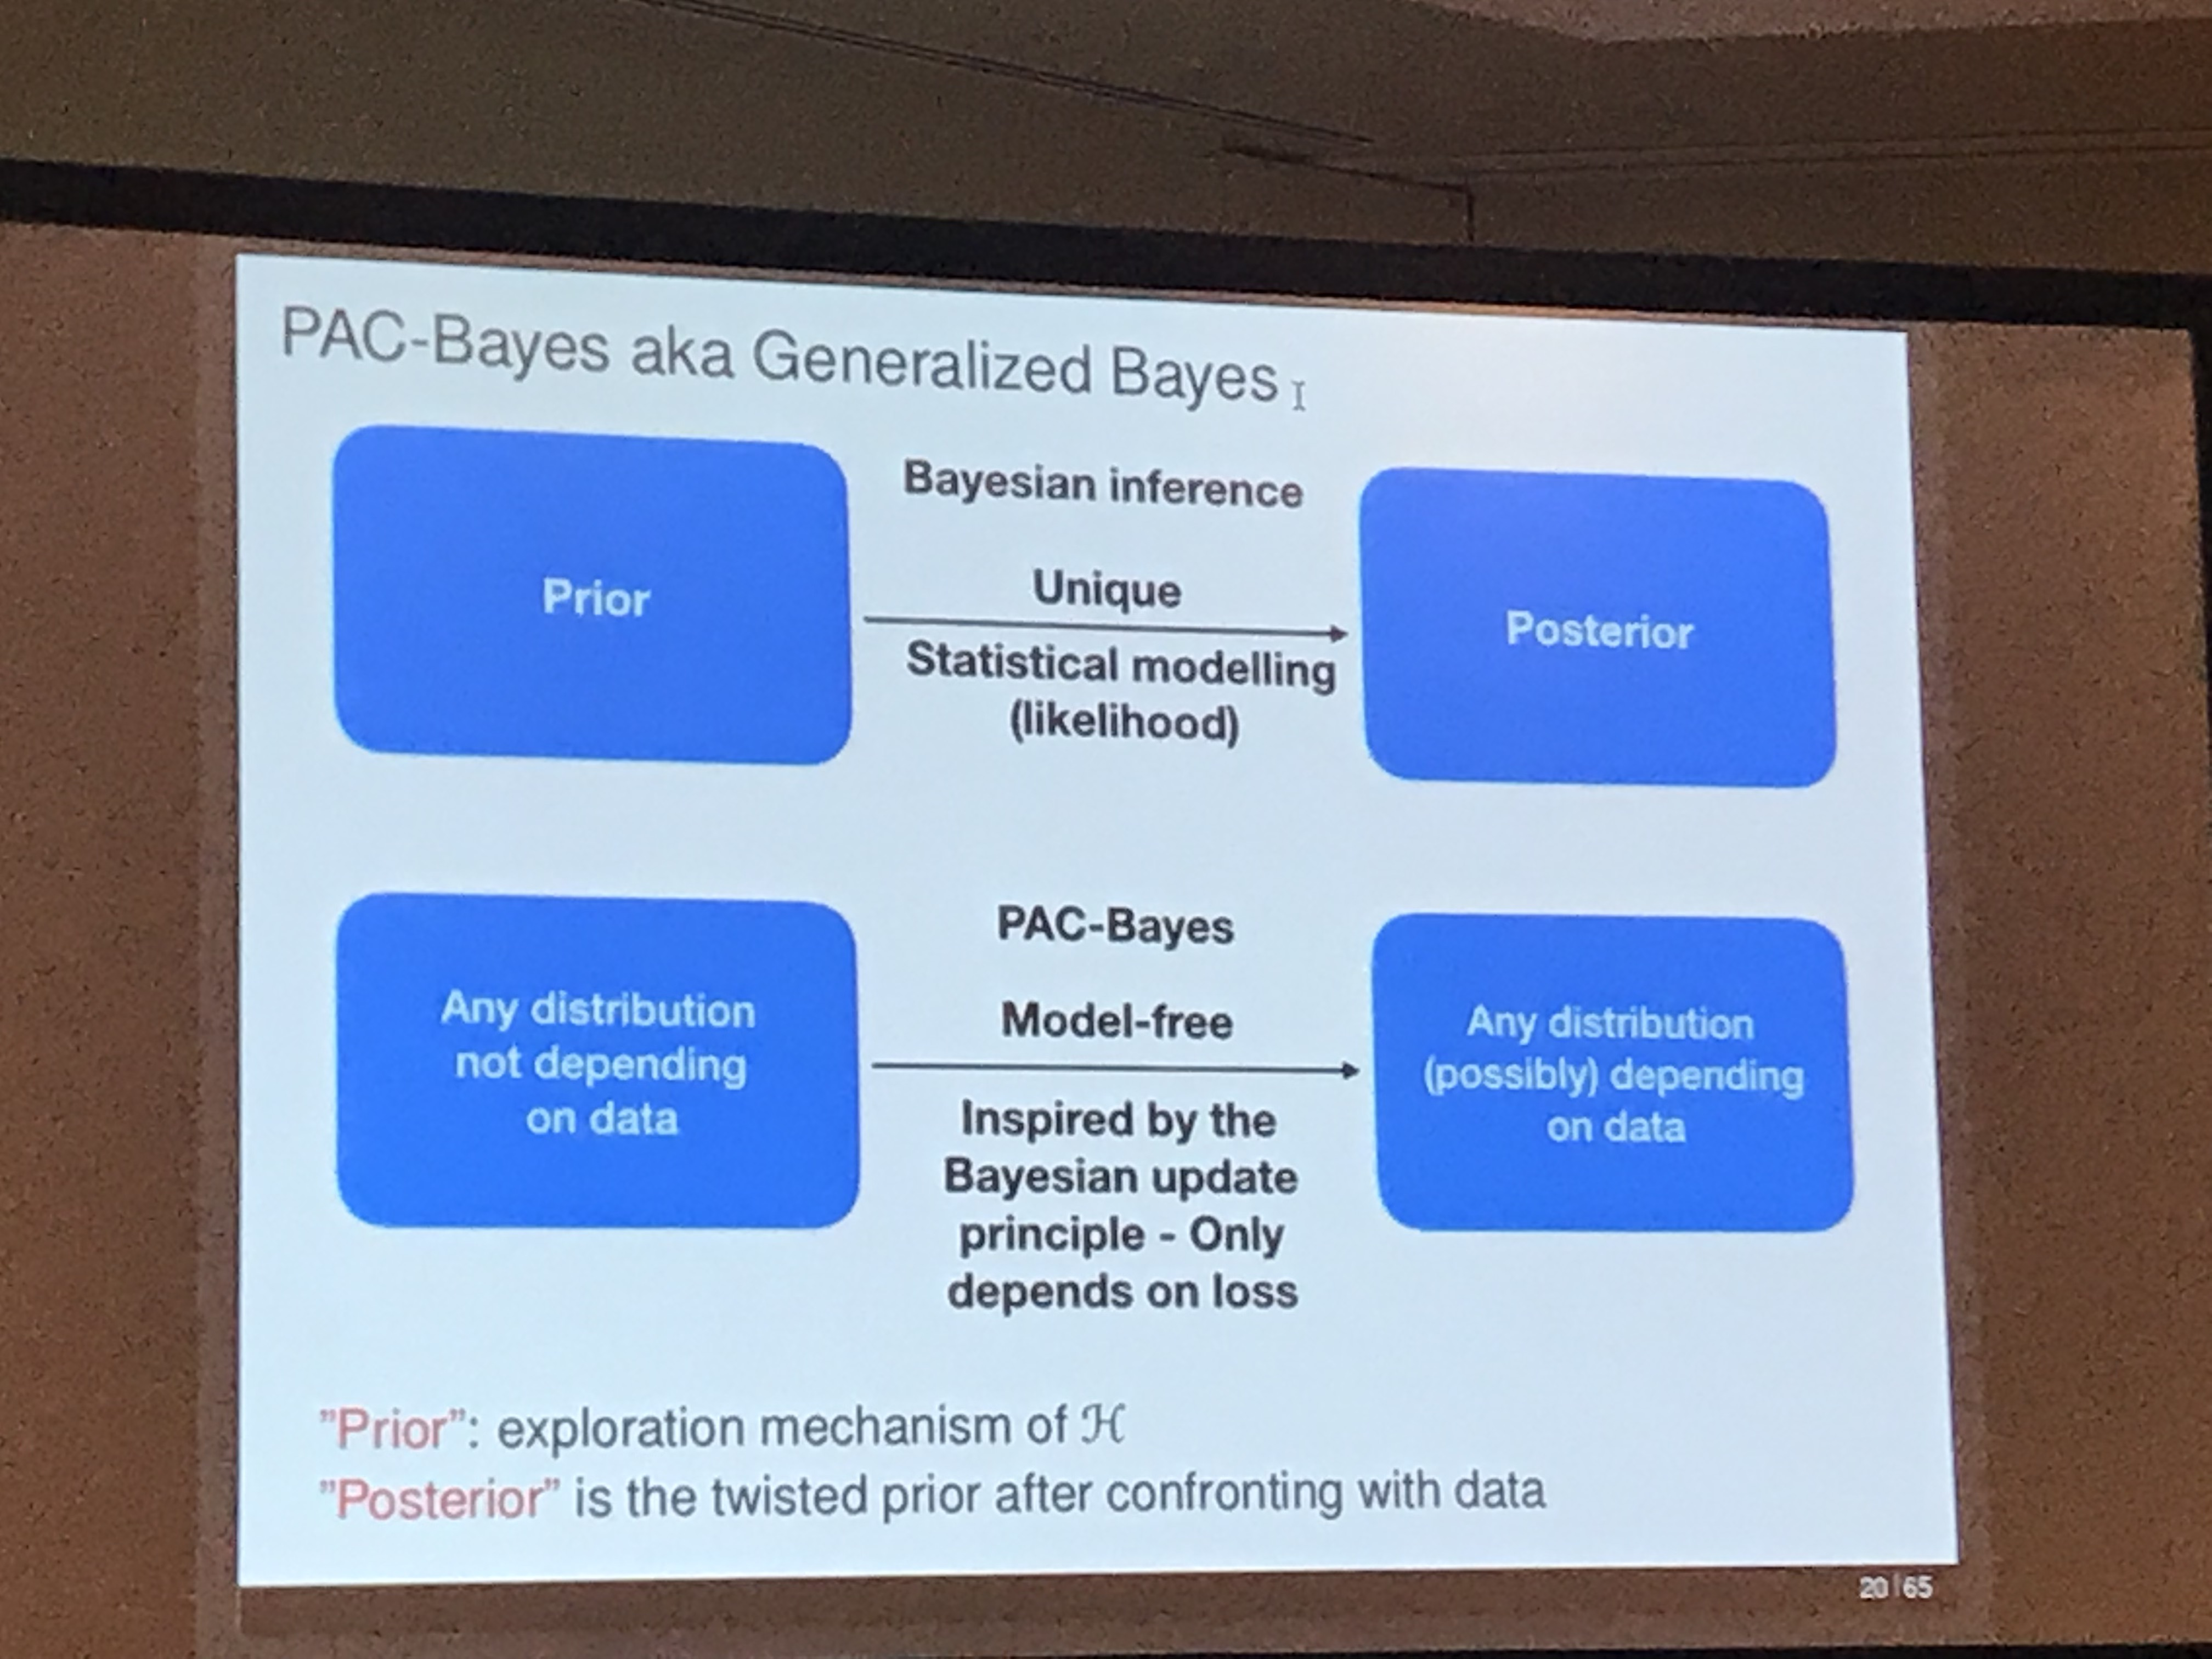
\includegraphics[width=0.5\textwidth]{images/pb1.JPG}
    \caption{Differences in Bayes and PAC-Bayes}
    \label{fig:pac_bayes}
\end{figure}


\begin{theorem}
\label{thm:pac_bayes}
(\citet{mcallester1999some}) For any prior $P$, $\delta \in (0,1]$, we have:
\begin{equation}
    \Pr\left(\forall_{Q \in \mc{H}} : R_{out}(Q) \leq R_{in}(Q) + \sqrt{\frac{\KL{Q}{P}) + \ln \frac{2 \sqrt{m}}{\delta}}{2m}}\right) \geq 1-\delta,
    \label{eq:pac_bayes}
\end{equation}
where $\mc{H}$ is the hypothesis space, $m$ is the number of samples, $R_{out}$ is the risk of a hypothesis on the test data, $R_{in}(h)$ is the risk of the data on the training data, $P$ is the prior, and $Q$ is the posterior.
\end{theorem}

PAC-Bayes: a flexible learning theoretic framework! Tight connections to regression, linear classification \& SVMs, transductive learning, uses in RL~\cite{fard2010pac}, and more.


\subsubsection{PAC-Bayes Theory}
This section explores the high level view of PAC-Bayesian Theory. \\

Q: How can PAC-Bayes drive learning? \\

A: First, recall:
\begin{equation}
    R_{out}(Q) \leq R_{in}(Q) + F(Q),
\end{equation}
Or:
\begin{equation}
    \text{Error on unseen data} \leq \text{Error on sample + complexity term}.
\end{equation}

This defines a principle strategy for obtaining new algorithms:
\begin{align}
    &h \sim Q^* \\
    &Q^* \in \text{arginf}_{Q \ll P} \left\{R_{in}(Q) + F(Q)\right\}.
\end{align}

Presents an optimization problem: can be solved or approximated to find good solutions! \\

PAC-Bayes interpretation of celebrated algorithms: 
\begin{itemize}
    \item SVM with a sigmoid loss and KL-regularized Adaboost canm be reinterpreted as minimizer of PAC-Bayesian bounds~\cite{ambroladze2007tighter}.
    \item Also, the minimizer of:
    \[
    \left\{R_{in}(Q) + \frac{KL}{\lambda}\right\},
    \]
    is the celbrated Gibbs posterior:
    \[
    Q_\lambda(h) \propto \exp(-\lambda R_{in}(h)) P9h), \hspace{5mm} \forall_{h \in \mc{H}}.
    \]
    
    When $\lambda \ra 0$, we get a flat posterior, and as $\lambda \ra \infty$, we get Dirac mass on expected risk minimization (ERMs).
\end{itemize}



\begin{theorem}
\[
\log \int (\exp \phi) dP = \sup_{Q \ll P} \left\{ \int \phi dQ - KL(Q,P)\right\}.
\]
\end{theorem}
\begin{proof}
First require variational definition of KL-Divergence~\cite{csiszar1975divergence}
\begin{align}
    -\KL{Q}{G} &= - \int \log\left(\frac{dQ}{dP} \frac{dP}{dG}\right) dQ \\
    &= -\KL{Q}{P} + \int \phi dp - \log \int(\exp \phi) dP.
\end{align}
Note that KL is non negative, $Q \ra -\KL{Q}{P}$ reaches its max in $Q=G$. Thus, taking $\phi = -\lambda R_{in}$:
\[
Q_\lambda(h) \propto \exp(-\lambda R_{in}(h)) P9h), \hspace{5mm} \forall_{h \in \mc{H}}. \qedhere
\]
\end{proof}

Q: What about non-i.i.d. data? \\

A: Sure! Let's drop the i.i.d. and bounded loss assumptions. First, consider the moment of a distribution:
\ddef{Moment}{The $p$-th moment of a distribution is given by:
\[
M_p := \int \bE\left[|R_{in}(h) - R_{out}(h)|^p )\right) dP(h).
\]}

Also make use of $f$-divergences, a generalization of the KL-Divergence. \\

\begin{theorem}
Let $\phi_p : x \mapsto x^p$. Fix $p > 1, q = \frac{p}{p-1}$ and $\delta \in (0,1)$. W/ probability at least $1-\delta$, for any distr. $Q$:
\[
|R_{out}(Q) - R_{in}(Q)| \leq (\frac{M_q}{\delta}^{1/q}(D_{\phi_{p-1}}(Q,P) + 1)^{1/p}.
\]
\end{theorem}

Takeaway: we can bound generalization error using the $f$-divergence ($D_{\phi_{p-1}}$ and moment $(M_q)$. Proof strategy requires: 1) Jensen's inequality, 2) change of measure, 3) Holder's inequality, and 4) Markov's inequality. \\

Oracle Bounds;~\citet{catoni2007pac} derived PAC-Bayesian bounds for the Gibbs posterior.

\subsubsection{PAC-Bayes and Task Awareness}

Note: PAC-Bayesian bounds express a tradeoff between empirical accuracy and a measure of complexity. \\

Q: So, how can we improve the bounds we get? How do we choose the right prior distribution so that we can 1) control complexity, and 2) ensure good performance? \\

$\ra$ So: can we choose a ``better' prior? (without looking at the test data itself?) \\

{\bf Main Idea:} use part of the data to learn how to choose a prior. \\

Can use PAC-Bayes in SVMs:
\begin{itemize}
    \item Assume prior and poster are spherical Gaussians (w/ prior centered at origin, posterirer centered at a scaling $\mu$ of unit SVM weight vector).
    \item Implies that KL term in generalization error bound is $\mu^2 / 2$ (see Theorem~\ref{thm:pac_bayes}).
    \item Can computer schochastic error of posterior distribution behaves like a soft margin, scaling $\mu$ trades between margin loss and KL.
    \item Bound holds for all $\mu$, so choose $\mu$ to optimize the bound.
\end{itemize}

Q: But how do we learn the prior for SVMs?
\begin{itemize}
    \item Bound depends on distance between prior and posterir
    \item Better prior means tighter bound
    \item Idea: learn prior $P$ with part of the data.
    \item Introduce learnt prior in the bound.
    \item Computer stochastic error with remaining data: PrPAC.
    \item Can go a step further: 1) scaling the prior in the chosen direction $\tau$-PrPAC, or 2) Adapt SVM to optimize the new bound: $\eta-$Prior SVM.
\end{itemize}

Results from the above methods for tightening the bounds: see Figure~\ref{fig:pb_results}. \\

\begin{figure}
    \centering
    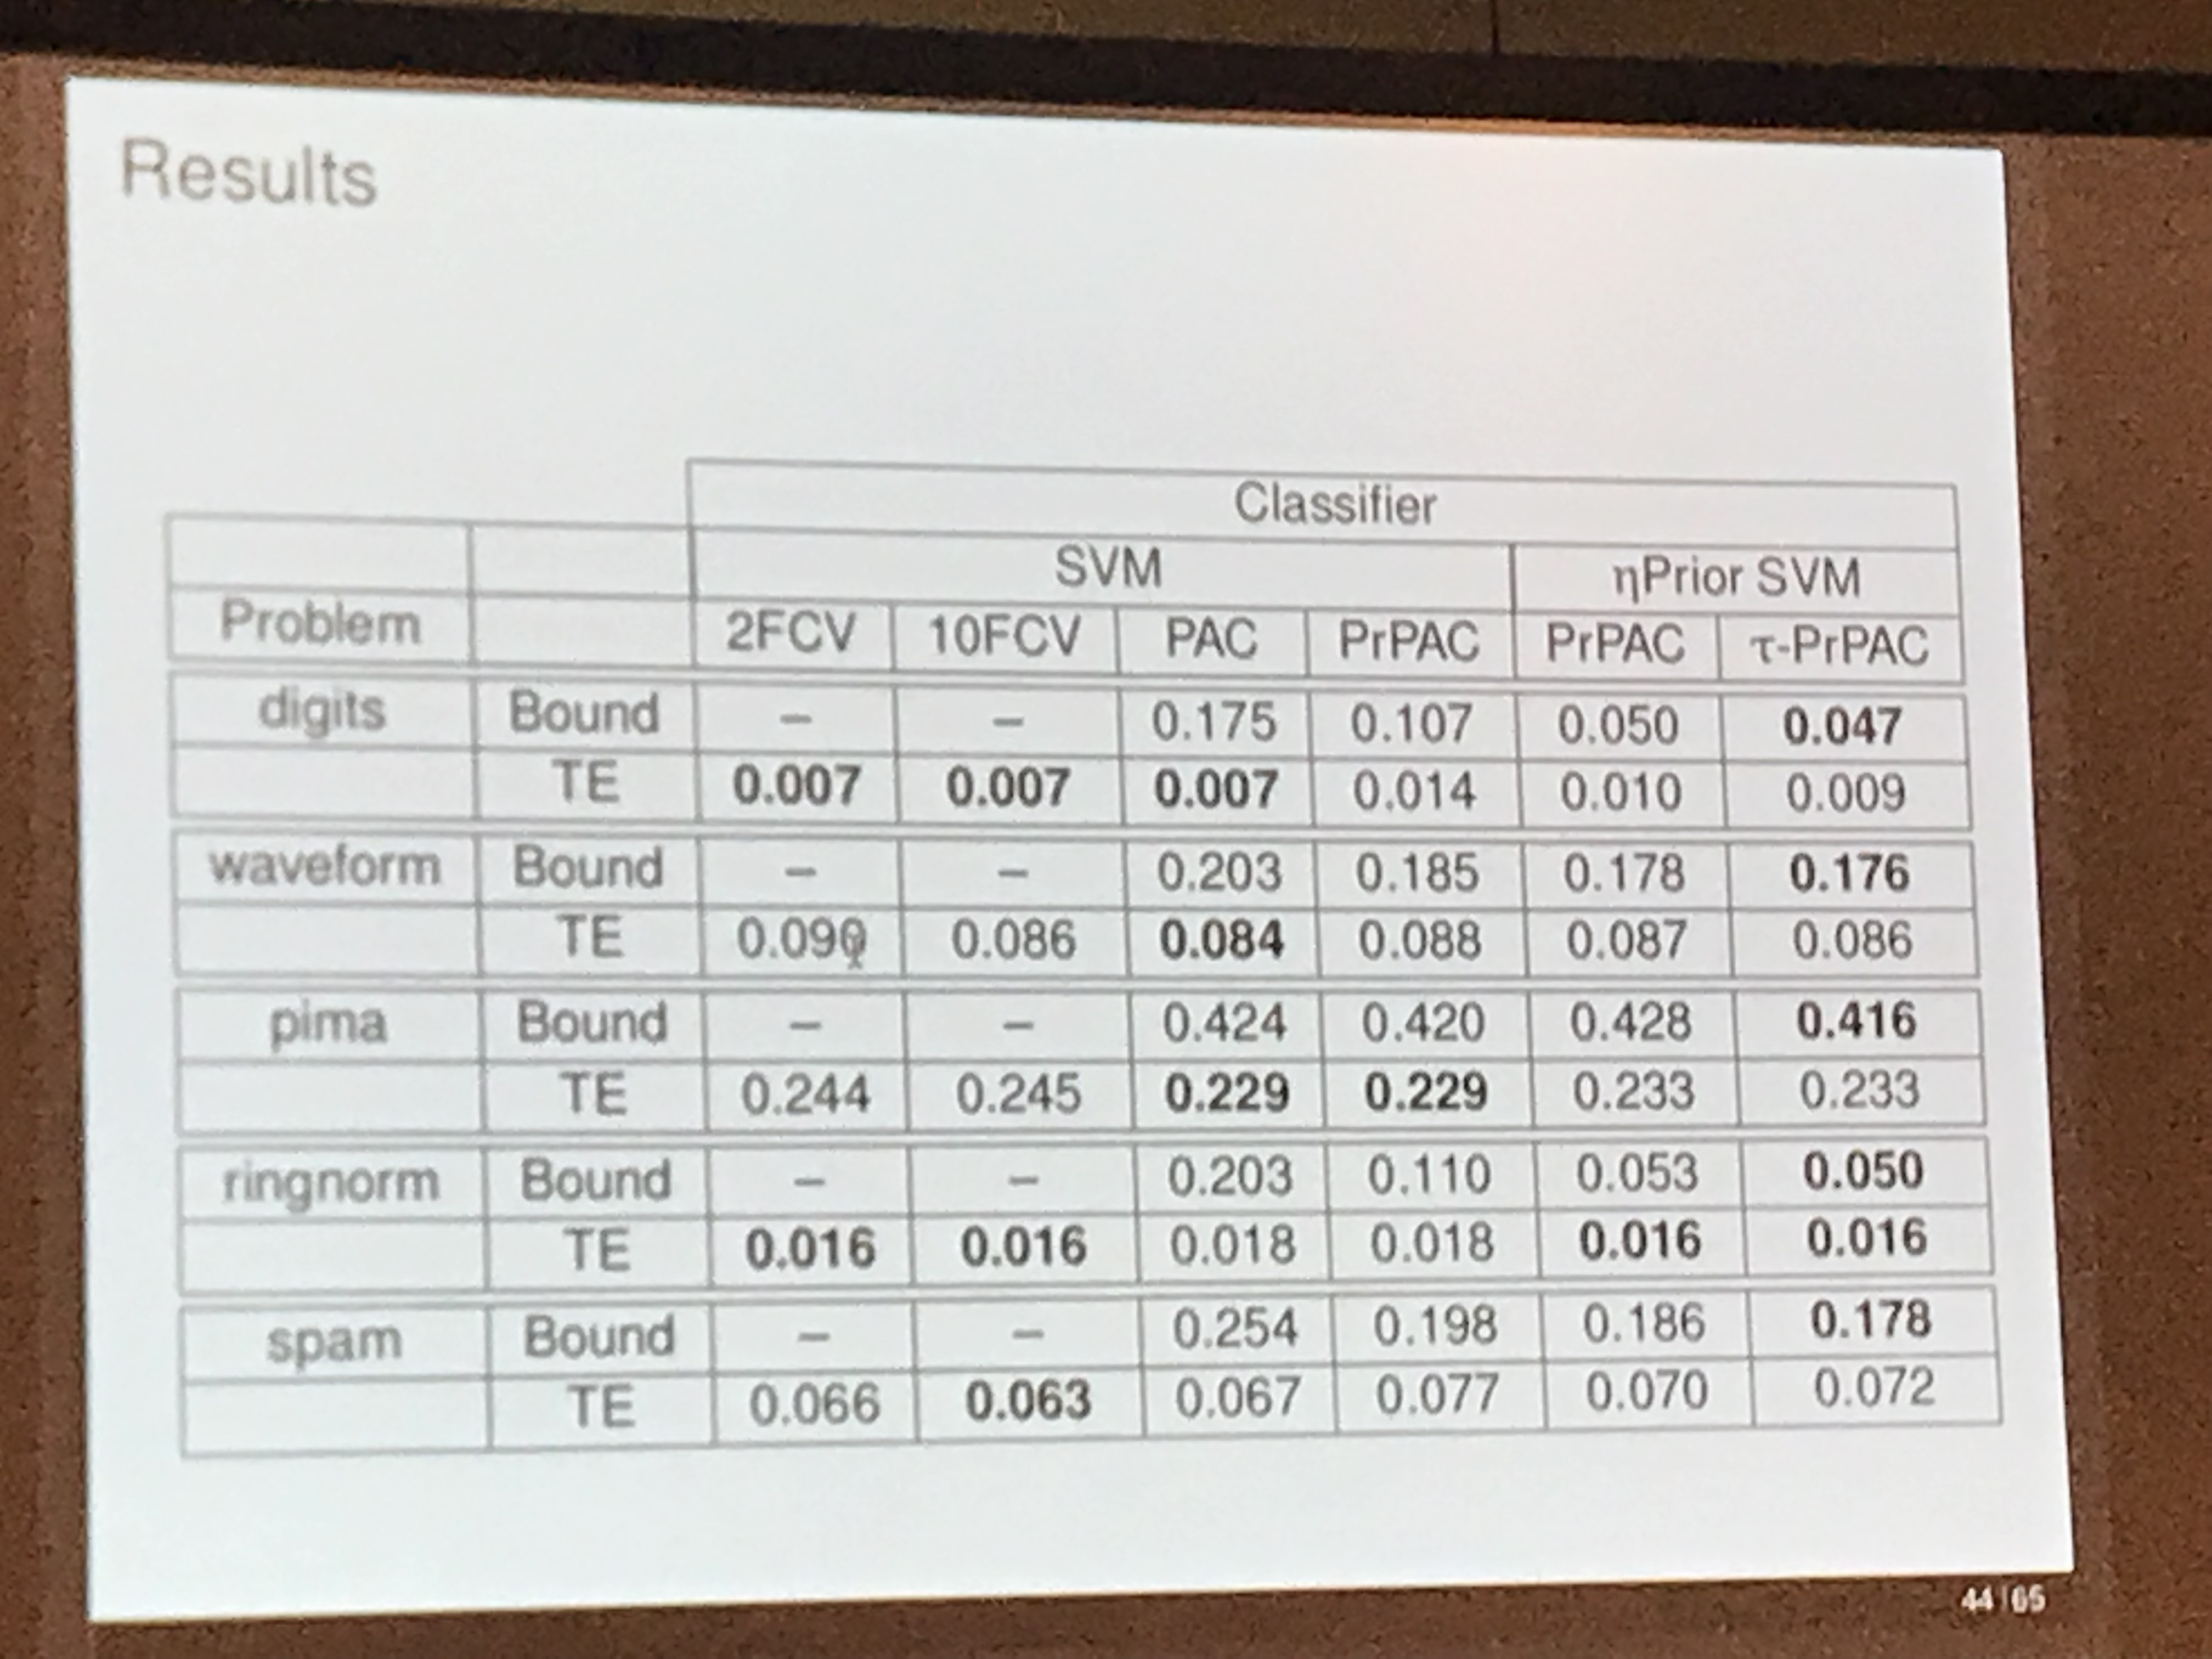
\includegraphics[width=0.5\textwidth]{images/pb_results.JPG}
    \caption{Results from applyinh differnet PAC-Bayes prior selection methods to experiments.}
    \label{fig:pb_results}
\end{figure}

Takeaways from results:
\begin{enumerate}
    \item Bounds are remarkably tight!
    \item Model-selection via these new bounds is {\it as good} as 10-fold cross validation.
    \item Best bounds don't necessarily translate into best model selection.
    
    $\ra$ We're not {\it completely} capturing the right thing (but definitely some of the right thing).
\end{enumerate}

Next up: distribution-defined priors:
\begin{itemize}
    \item Consider $P$ and $Q$ are Gibbs-Boltzmann distributions:
    \[
    P_\gamma(h) = \frac{1}{Z} \exp(-\gamma R_{out}(h) \hspace{8mm} Q_\gamma(h) = \frac{1}{Z}\exp(-\gamma R_{in}(h)).
    \]
    \item These distributions hard to work with since we can't apply it to a single weight vector. From~\citet{catoni2007pac}, we can show:
    \[
    \KL{R_{in}(Q_\lambda)}{R_{out}(Q_\lambda)} \tilde{\leq} \frac{1}{m} \left(\gamma / \sqrt{m} + \gamma^2/4m\right),
    \]
    where $\tilde{\leq}$ ignores log terms on the right hand side (\dnote{my (awful) construction for abbreviation, not theirs}).
    
\end{itemize}

On stability:
\begin{itemize}
    \item If $A$ has sensitivity $\beta$ at sample size $m$, then generalization error can be bounded~\cite{bousquet2002stability}.
    
    \item Q: Algorithm output is highly concentrated, does that imply stronger results?
    
    $\ra$ Yes! We can derive (tighter) bounds that depend on KL between a distributionally sensitive prior and a well chosen posterior.
    
    Open area! Lots of room to explore a new kind of generalization error analysis.
\end{itemize}

{\bf A final case study:} Can we use any of this to analyze deep neural networks? \\

Q: Is deep learning breaking the statistical paradigm we know? \\

$\ra$ Neural nets trained on massive datasets achieve {\it zero training error}, which does not bode well for their performance. Yet! They tend to achieve remarkably low error on test sets, too. \\

{\bf Idea:} Perhaps we can use PAC-Bayes to explain this phenomena. \\



\begin{figure}
    \centering
    \subfloat[Classical view of Overfitting]{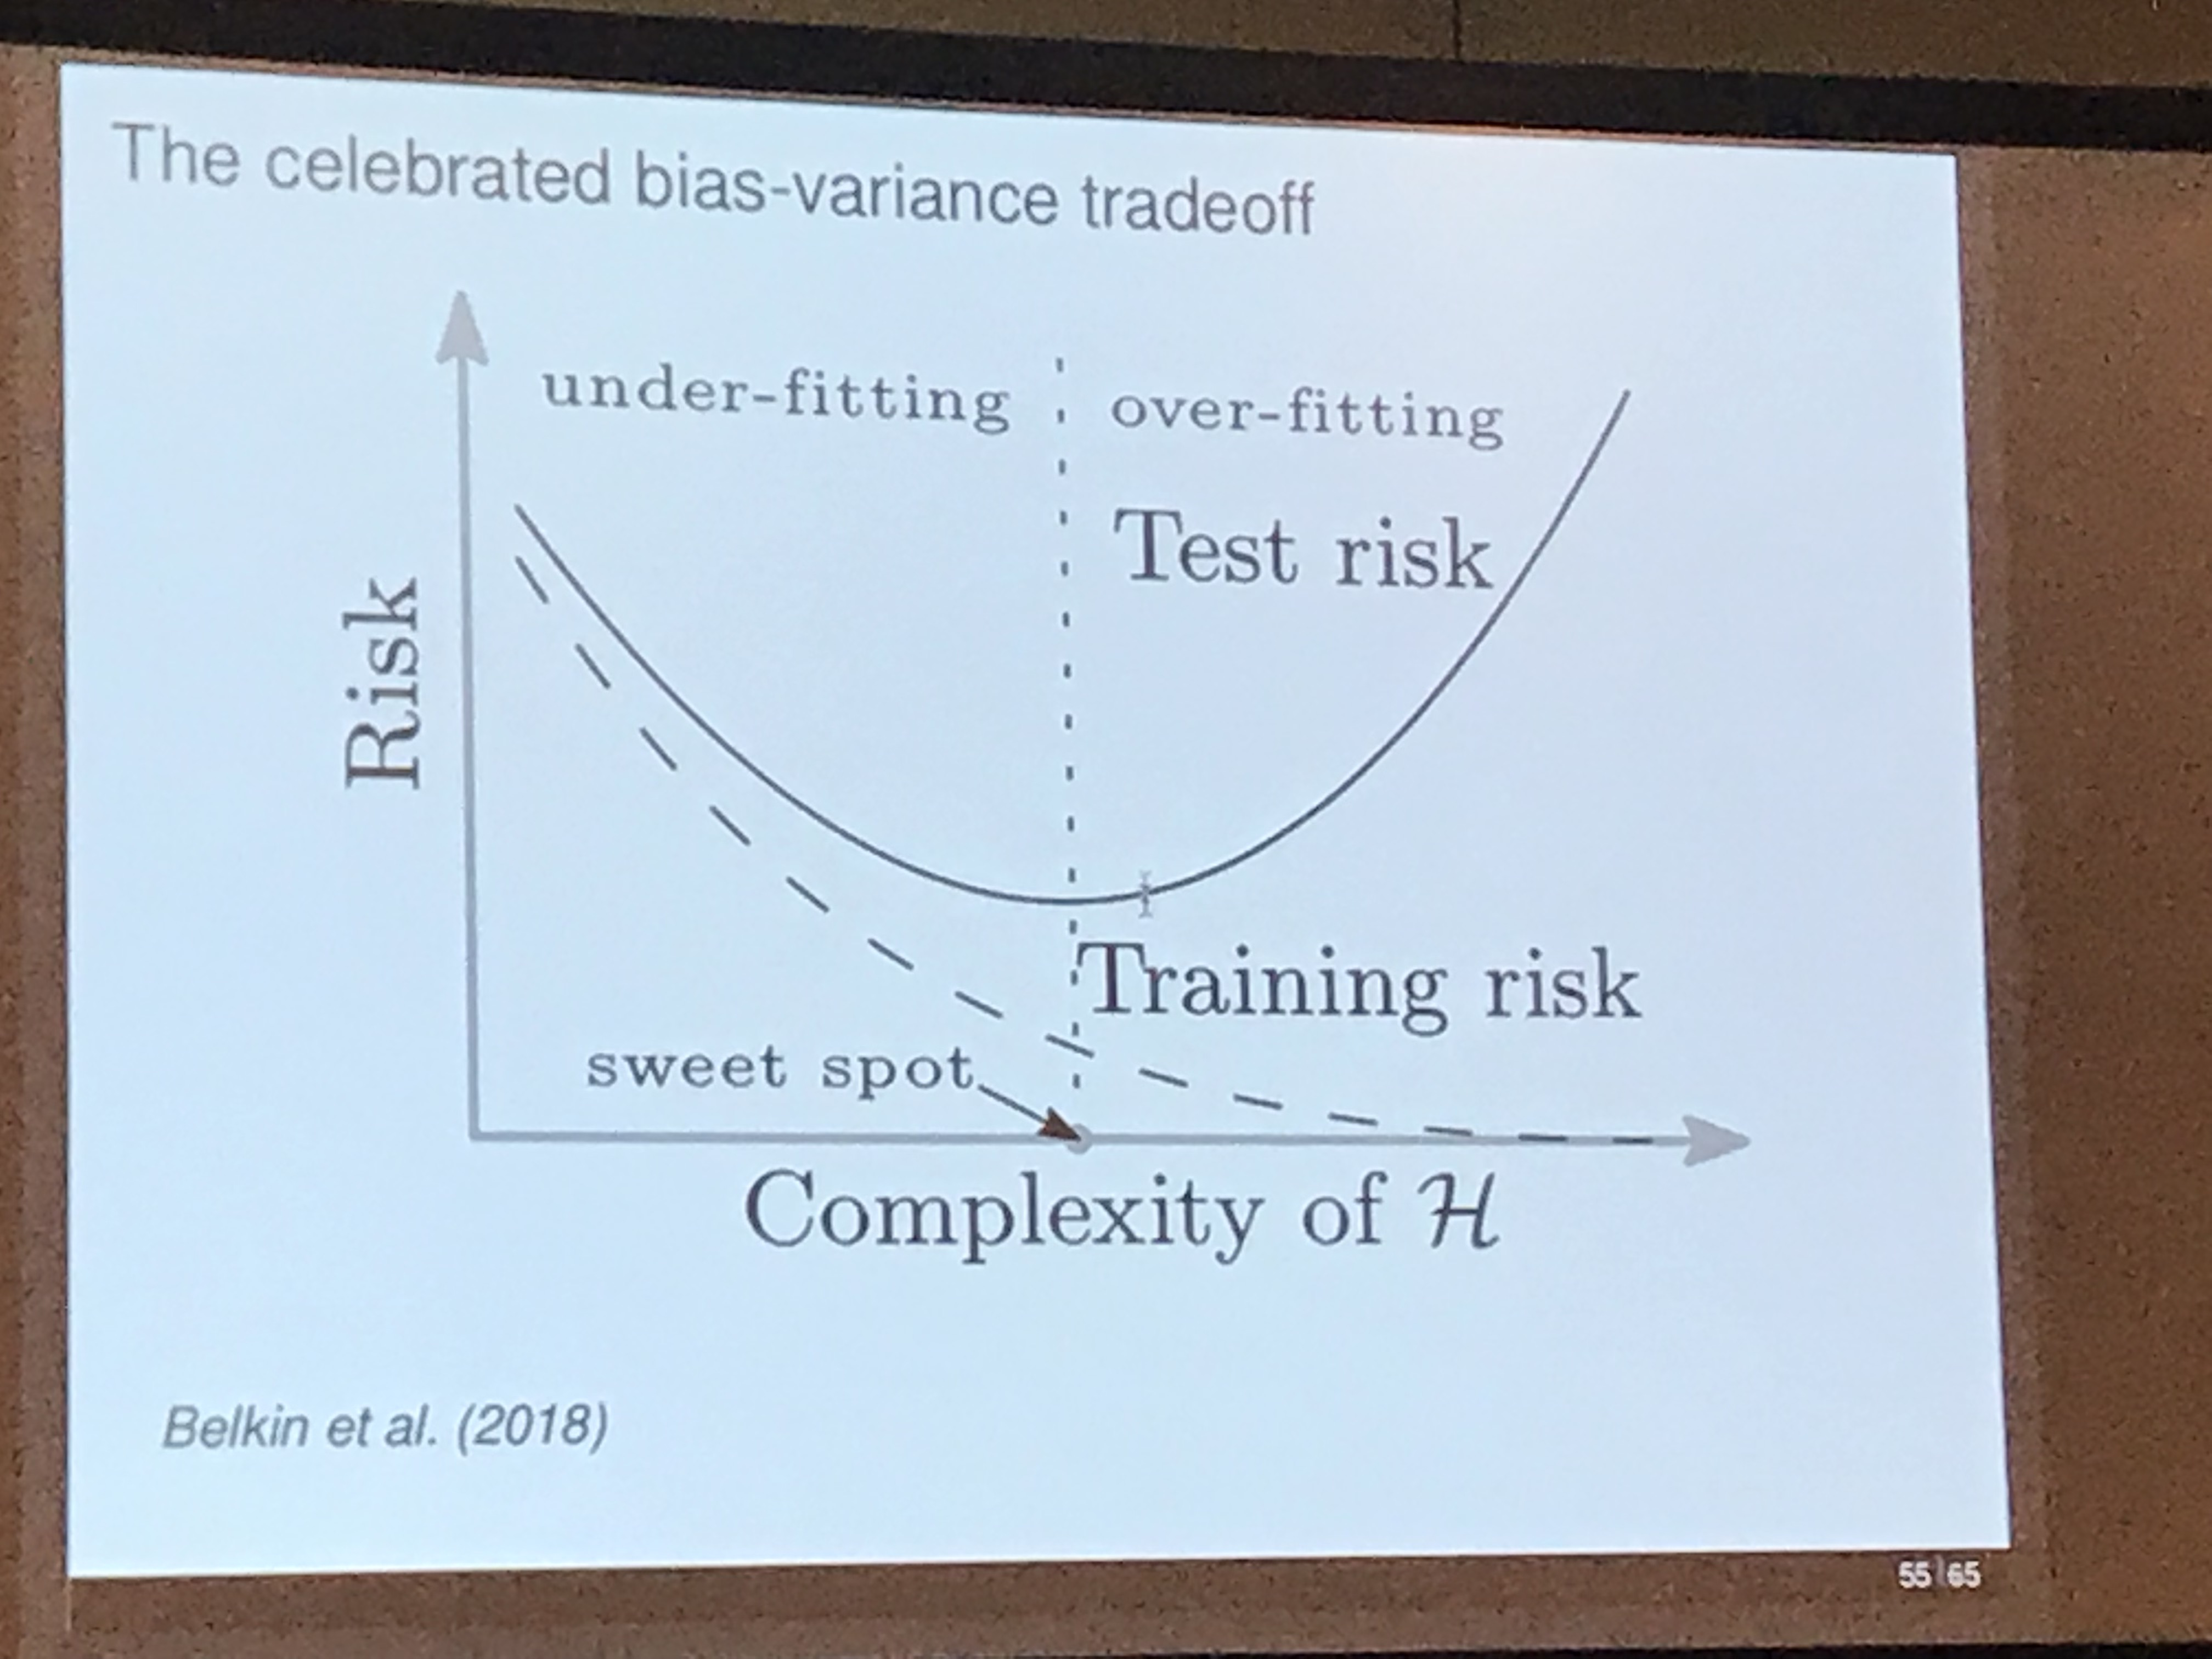
\includegraphics[width=0.45\textwidth]{images/of.JPG}} \hspace{2mm}
    \subfloat[New Paradigm?]{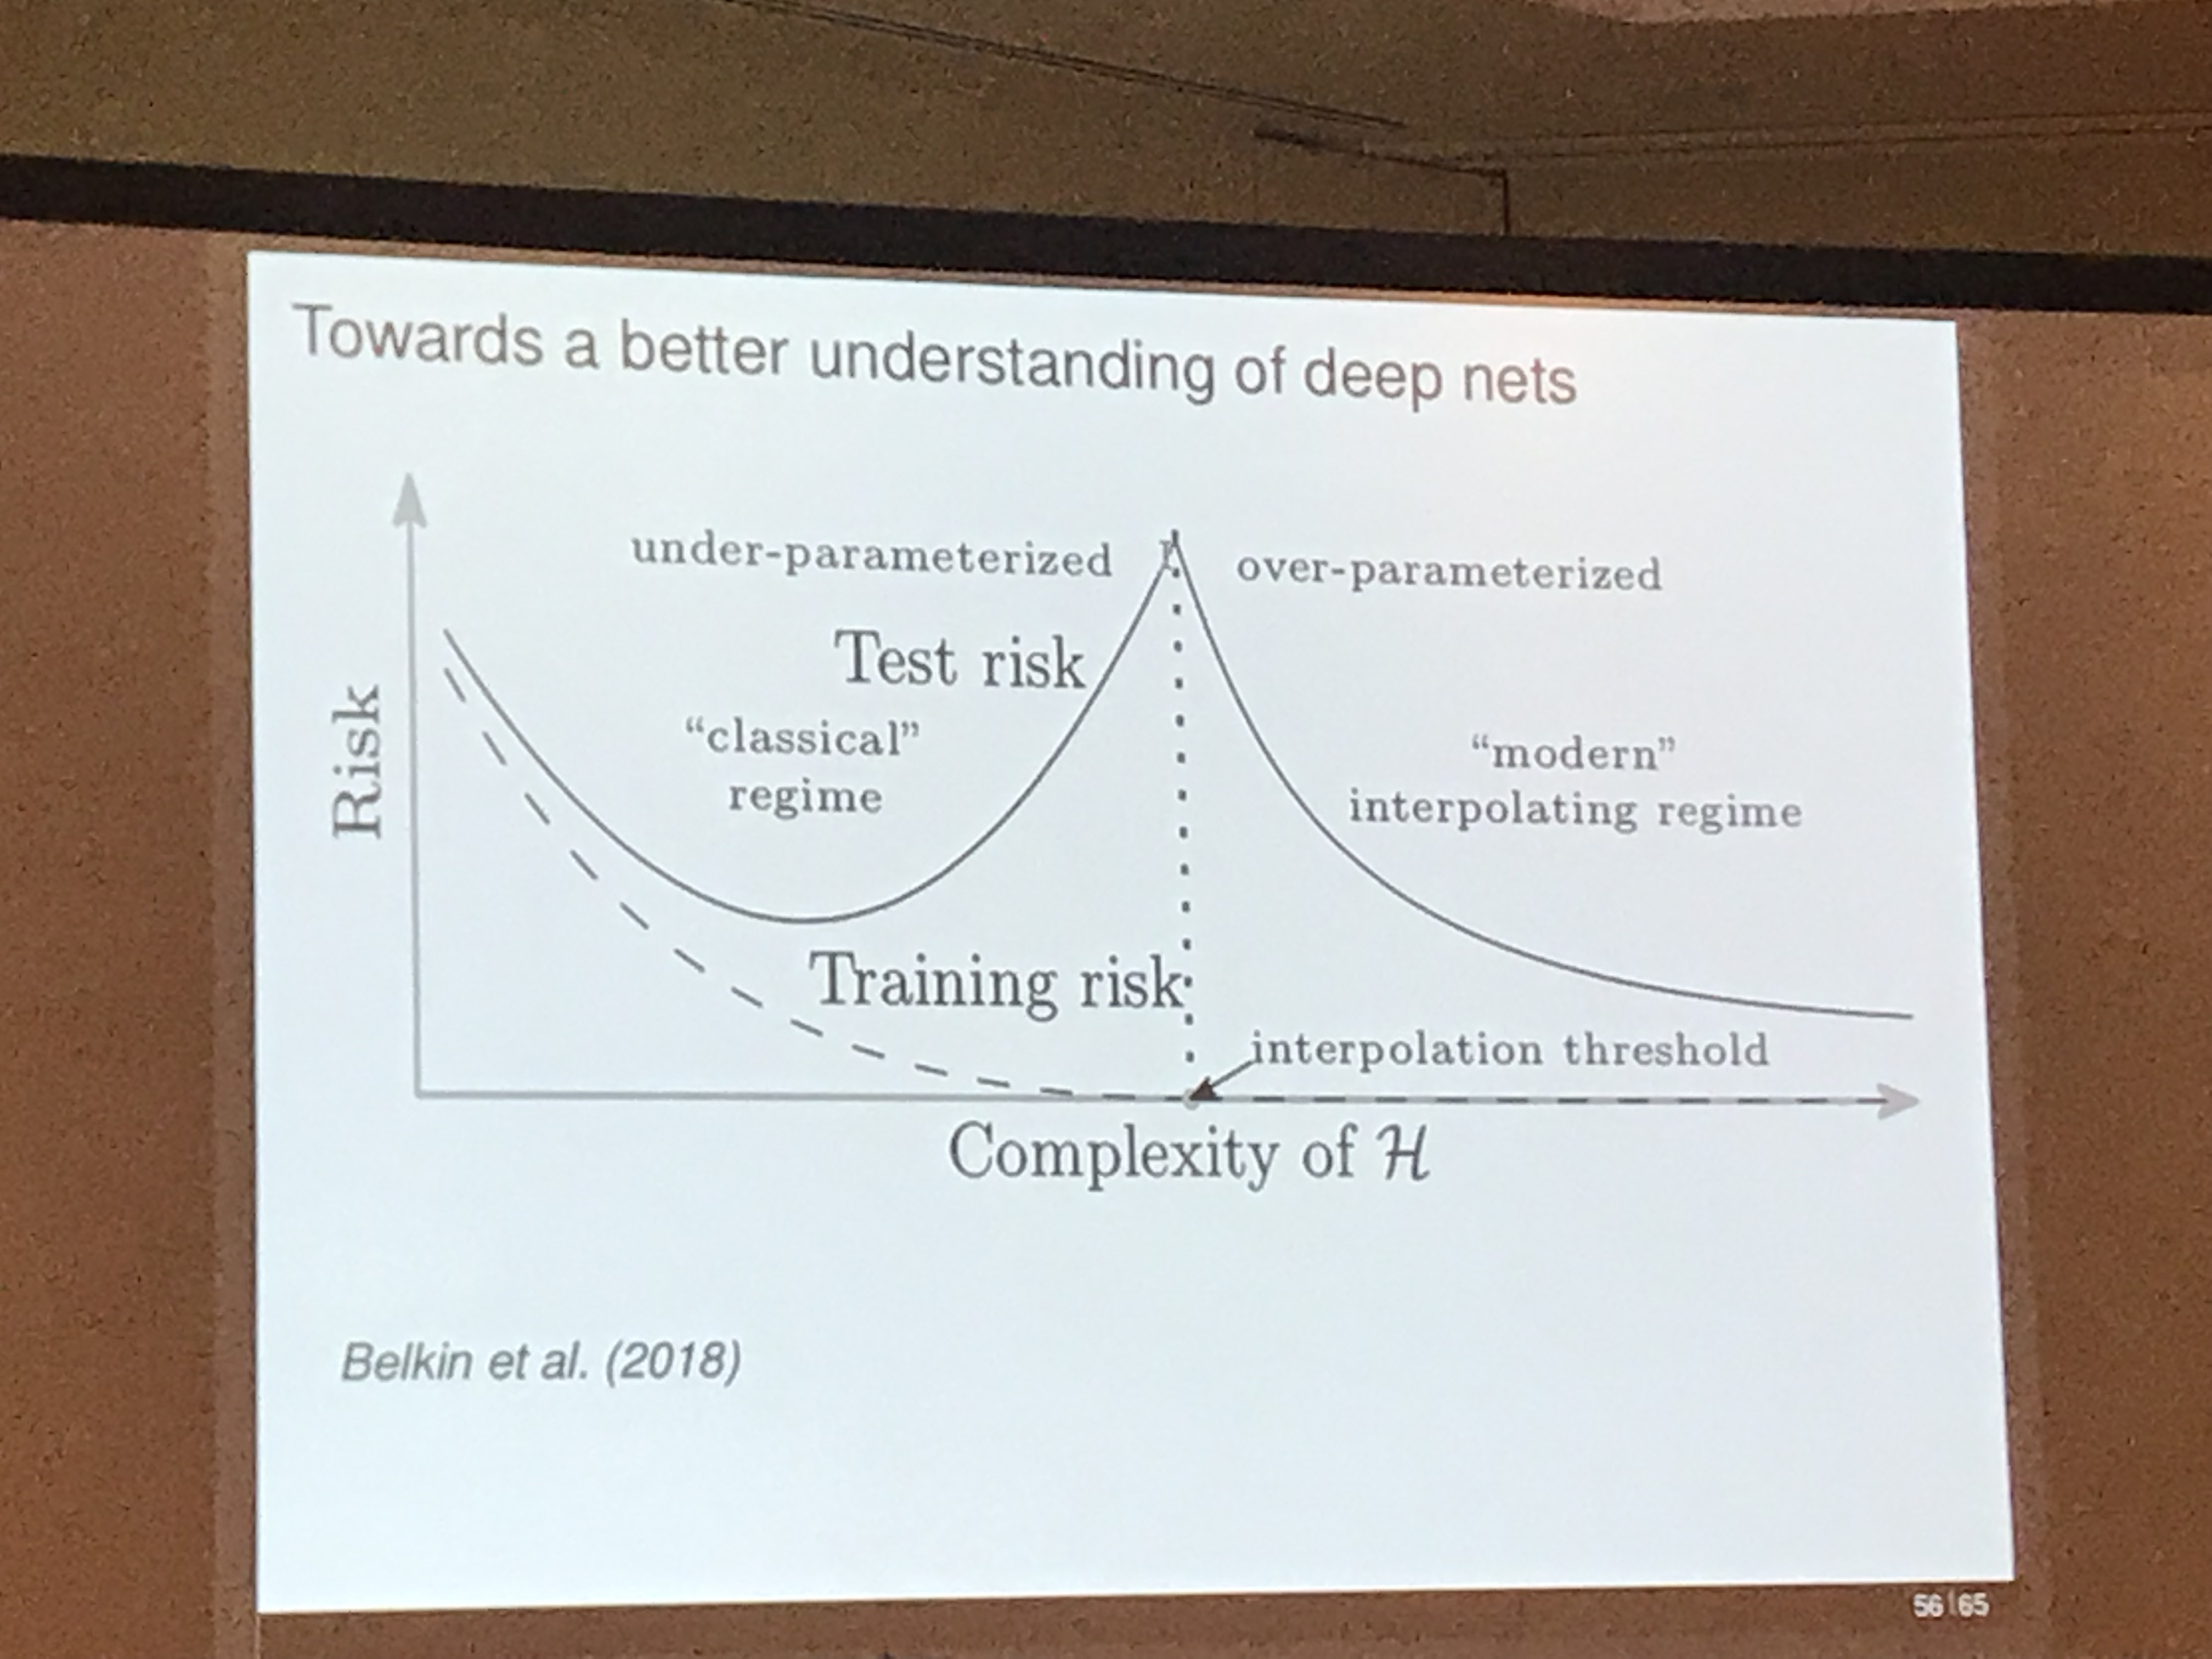
\includegraphics[width=0.45\textwidth]{images/of_2.JPG}}
    \caption{Classical view of overfitting (left), and a new proposal for why deep nets might be avoiding overfitting (right), from~\citet{belkin2018overfitting}.}
    \label{fig:overfitting}
\end{figure}

~\citet{dziugaite2017entropy} derived extremely tight deep learning generalization error bounds in this way;
\begin{itemize}
    \item Based on training to expand the ``basin of attraction"
    \item Hence, not measuring good generalization of {\it normal training}
\end{itemize}

Q: How much information is contained in the training set? \\

A1: ~\citet{achille2018information} studied the {\it amount of information} stored in the weights of deep networks. Overfitting might be related to information being stored in weights that encode training set, as opposed to the data generation distribution. \\

A2: Information bottleneck criterion~\cite{} might control this information, and could lead to a tighter PAC-Bayes bound. \\

{\bf Conclusions:}
\begin{itemize}
    \item PAC-Bayes arises from two fields: 1) statistical learning theory, and 2) Bayesian Learning
    \item Generlazies both fields and points to promising directions
    \item PAC-Bayes theory can be an inspiration toward new theoretical analysis, but also drive algorithm design (especially when theory has proven difficult).
\end{itemize}


\subsection{Tutorial: Meta-Learning}

The speakers are Chelsea Finn and Sergey Levine. \\

{\bf Motivation:} Learn from small amounts of data. \\

$\ra$ Recent advancements {\it thrive} in large diverse data sets 9in the sense that it allows for broad generalization) (see; BERT, AlexNet0 \\

$\ra$ Existing approaches require huge data sets. But, some questions:
\begin{enumerate}
\item  what if we don't have a large dataset/
\item What if we want a general purpose AI system in the world?
\item What if our data has a long tail?
\end{enumerate}

Point: these settings start to break the standard supervised learning setting. \\

Example: few shot learning with painting, people (the audience) was able to ``generalize" to guess the painter of a new painting. \\

Q: How do we accomplish this? \\

A: Well, previous experience! We weren't really doing this based on no prior experiences. We have encountered similar questions/tasks/images before. \\

Q: How might we get a machine to accomplish this task?  \\

A: Well, we might encode structure via: $\{$modeling image formation, geometry, task-specific features, hyperparameter choice$\}$, and so on \\

\dbox{{\bf Main Point:} Can we explicitly learn priors from previous experience that lead to efficient downstream learning?}

Outline:
\begin{itemize}
\item Problem statement
\item Meta-Learning Algorithms
\item Meta-Learning Applications
\item Meta-Reinforcement Learning
\end{itemize}

\subsubsection{Two Ways to View meta-Learning}

Q: How do we formulate the meta-learning problem? \\

A1: Mechanistic view! A model reads in an entire data set and makes predictions for new datapoints. Training this network uses a ``meta"-dataset which itself consists of many datasets. \\

A2: Probabilistic view: expreact prior info from a set of (meta-training) tasks that allows efficient learning of tasks. Learning a new task usis this prior training set to infer most likely posterior parameters. \\

$\ra$ A1 is more convenient for implementation, A2 is more convenient for understanding. \\

\ddef{Supervised Learning}{Find the parameters $\phi$ given data $D$:
\[
\argmax_{\phi} \Pr(\phi \mid D),
\]
where $D = \{(x_1,y_1), \ldots, (x_n, y_n)\}$. Applying Bayes rules, this comes out to:
\[
\argmax_{\phi} \log \Pr(D \mid \phi) + \Pr(\phi).
\]
}
\ddef{Meta-Learning}{Find the parameters $\theta$ that enables us to quickly solve new tasks, given a bunch of datasets $D_{\text{meta-train}}$:
\[
\argmax_{\phi} \log \Pr(\phi \mid D, D_{\text{meta-train}} = \argmax_{\theta} \log \int_\Theta \Pr(\phi \mid D, \theta) \Pr(\theta \mid D_{\text{meta-train}}.
\]
That is, we assume $\theta$ are the sufficient statistics for $\phi$. 
}
Hard to perform this decomposition in general: usually take a Maximum A Posteriori (MAP) approach. \\

{\bf Goal of Meta-Learning:} Find an appropriate set of parameters $\theta$, that are maximially probable given the meta-datasets. So:
\[
\theta^* = \argmax_\theta \log \Pr(\theta \mid D_{\text{meta-train}}.
\]

Notably, $D_{\text{meta-train}}$ might consist of {\it different} tasks (with related structure). \\

{\bf Example:} Want to classify new data sets. First, do meta learning;
\[
\theta^* = \argmax_\theta \log \Pr(\theta \mid D_{\text{meta-train}}.
\]
Then, adapt and find some nearby parameters, $\phi^*$:
\[
\phi^* = \argmax_{\phi} \log \Pr(\phi \mid D, \theta^*).
\]


{\bf Key Idea;} Our training procedure is based on a simple machine learning principle: test and train conditions much match" (from Vinyals et al. Matching Networks for One Shot learning). \\

Thus, for our above notion of meta-learning to make sense, we also need to hang on to tests {\it for each training} task. See Figure. \dnote{ADD FIG}. \\

Therefore, meta-learning can be written as:
\[
\theta^* = \max_\theta \nsum \log \Pr(\theta_i \mid D_i^{\text{test}}.
\]

\begin{figure}
    \centering
    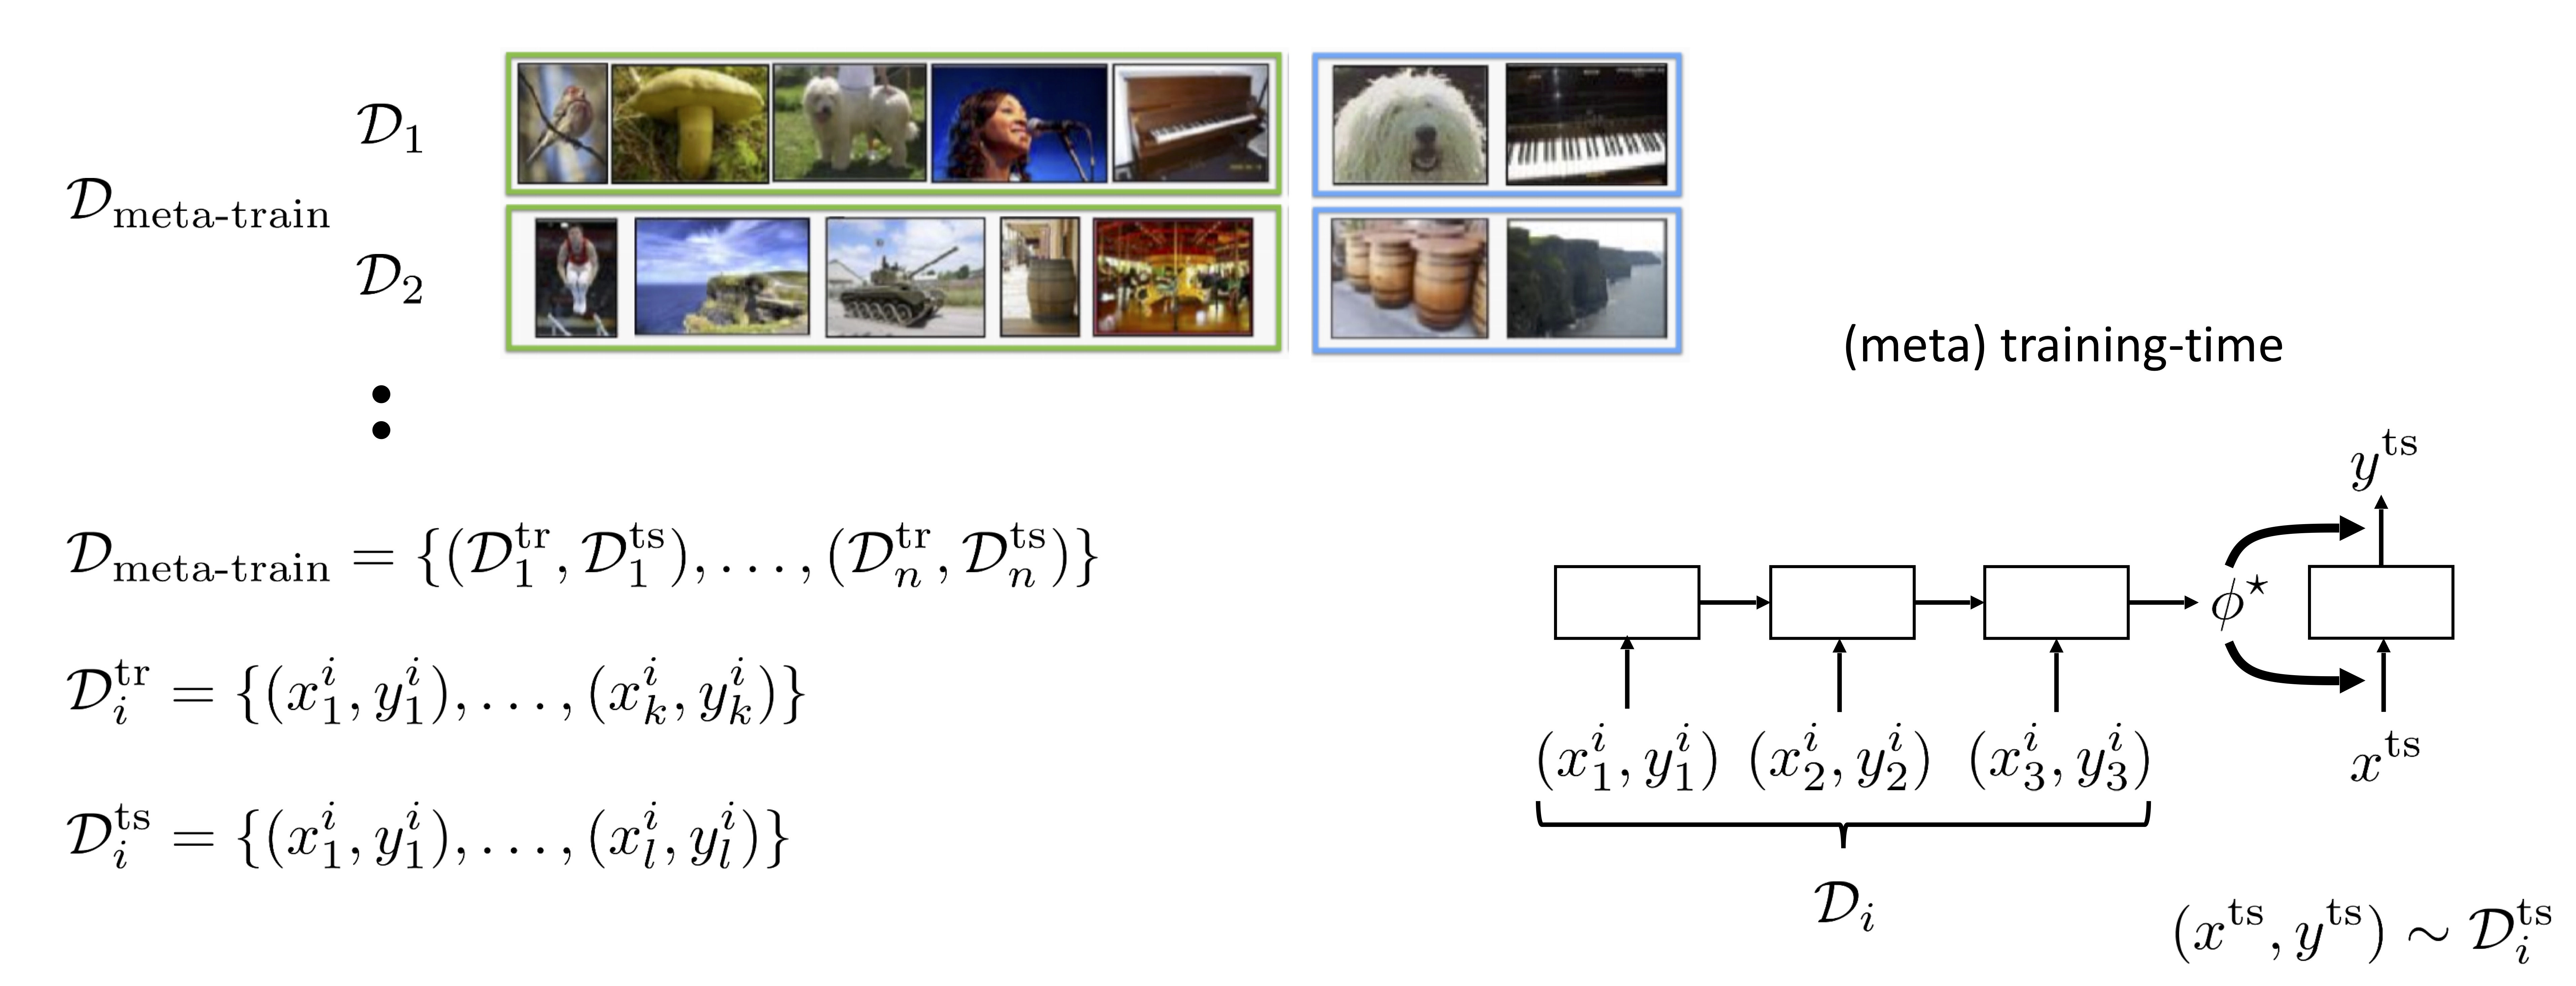
\includegraphics[width=0.75\textwidth]{images/meta_learn_1.jpg}
    \caption{Meta Learning paradigm}
    \label{fig:meta_learn}
\end{figure}

{\bf Closely related problem settings:}
\begin{enumerate}
\item Multi-task learning: special case of meta-learning where $\theta = \phi$.
\item Hyperparameter optimization: can also be cast as meta-learning with $\theta$=hyperparameters and $\phi$=network weights.
\end{enumerate}

\subsubsection{Meta-Learning Algorithms}

Before discussing algorithms, let's discuss {\it evaluation}. \\

{\bf Main Idea:} See~\citet{lake2015human}, introduced the Omniglot dataset. Idea: lots of classes, few examples of each class. Consists of 1623 characters from 50 different alphabets, 20 instances of each character. \\

$\ra$ Proposes both few-shot discriminative and few-shot generative problems. Initial few-short learning approaches w/ Bayesian models, non-parameterics. Other such databsets: CIFAR, CUB, MiniImageNEt. \\

Q: How do we evaluate a meta-learning algorithm? \\

A: Perform usual meta-training, and determine whether the resulting model can still perform quick generalization across different (held-out) tasks. \\

{\bf **General Recipe for Meta-Learning Algorithms:}
\begin{enumerate}
\item Choose a form of $\Pr(\phi_i \mid D_i^{\text{train}}, \theta)$.
\item Choose how to optimize $\theta$ with respect to max-likelihood objective using $D_{\text{meta-train}}$.
\end{enumerate}

Approach 1: Black-box adaptation. Key idea is to train a {\it neural net to represent} $\Pr(\phi_i \mid D_i^{\text{train}}, \theta)$. \\

$\ra$ For instance, might use an RNN to represent $f_\theta$, given a bunch of these meta-training datasets. Then, we can train with standard supervised learning:
\[
\max_\theta \sum_{T_i} L(f_\theta(D_i^{\text{train}}, D_i^{\text{test}})).
\]

{\bf Challenge:} Outputting all neural net parameters does not seem scalable
$\ra$ But, we don't need to output all parameters of a neural not, just the sufficient statistics. \\

Q: How can we frame this as an optimization procedure? \\

Approach 2: Acquire $\phi_i$ through optimization:
\[
\max_{\phi_i} \log \Pr(D_i^{\text{train}} \mid \phi_i) + \log \Pr(\phi_i \mid \theta).
\]
Meta-parameters $\theta$ serve as a {\it prior}. What form of prior? One form that has been successful: learn $\theta$ from {\it other tasks}. \\

{\bf Goal:} Learn a parameter vector $\theta$ that will transfer effectively, in the sense that it makes fine-tuning on new tasks easy/useful. To do so, solve the following problem;
\[
\min_\theta \sum_i L(\theta - \alpha \nabla_\theta L(\theta, D_i^{\tx{train}}), D_i^{\tx{test}}).
\]
General algorithm:
\begin{enumerate}
\item Sample task $T_i$.
\item Sample disjoint data sets from $D_i$
\item Optimize $\phi_i \la \theta - \alpha \nabla_\theta L(\theta, D_i^{\tx{tr}})$
\item Update $\theta$ using $\nabla_\theta L(\theta, D_i^{\tx{train}})$.
\end{enumerate}

So, we're left with two approaches: Optimization vs. Black-Box Adaptation \\

$\ra$ Model-Agnostic Meta-Learning (MAML), in the optimization can, can be viewed as a computation graph with embedded gradient operator (see Figure~\ref{fig:maml}:
\begin{align}
 y^{ts} &= f_{\tx{MAML}}(D_i^{\tx{train}}, x^{\tx{test}} \\
 &= f_{\phi_i}(x^{ts}),
\end{align}
where $\phi_i = \theta - \alpha \nabla_\theta L(\theta, D_i^{\tx{train}})$.

\begin{figure}
    \centering
    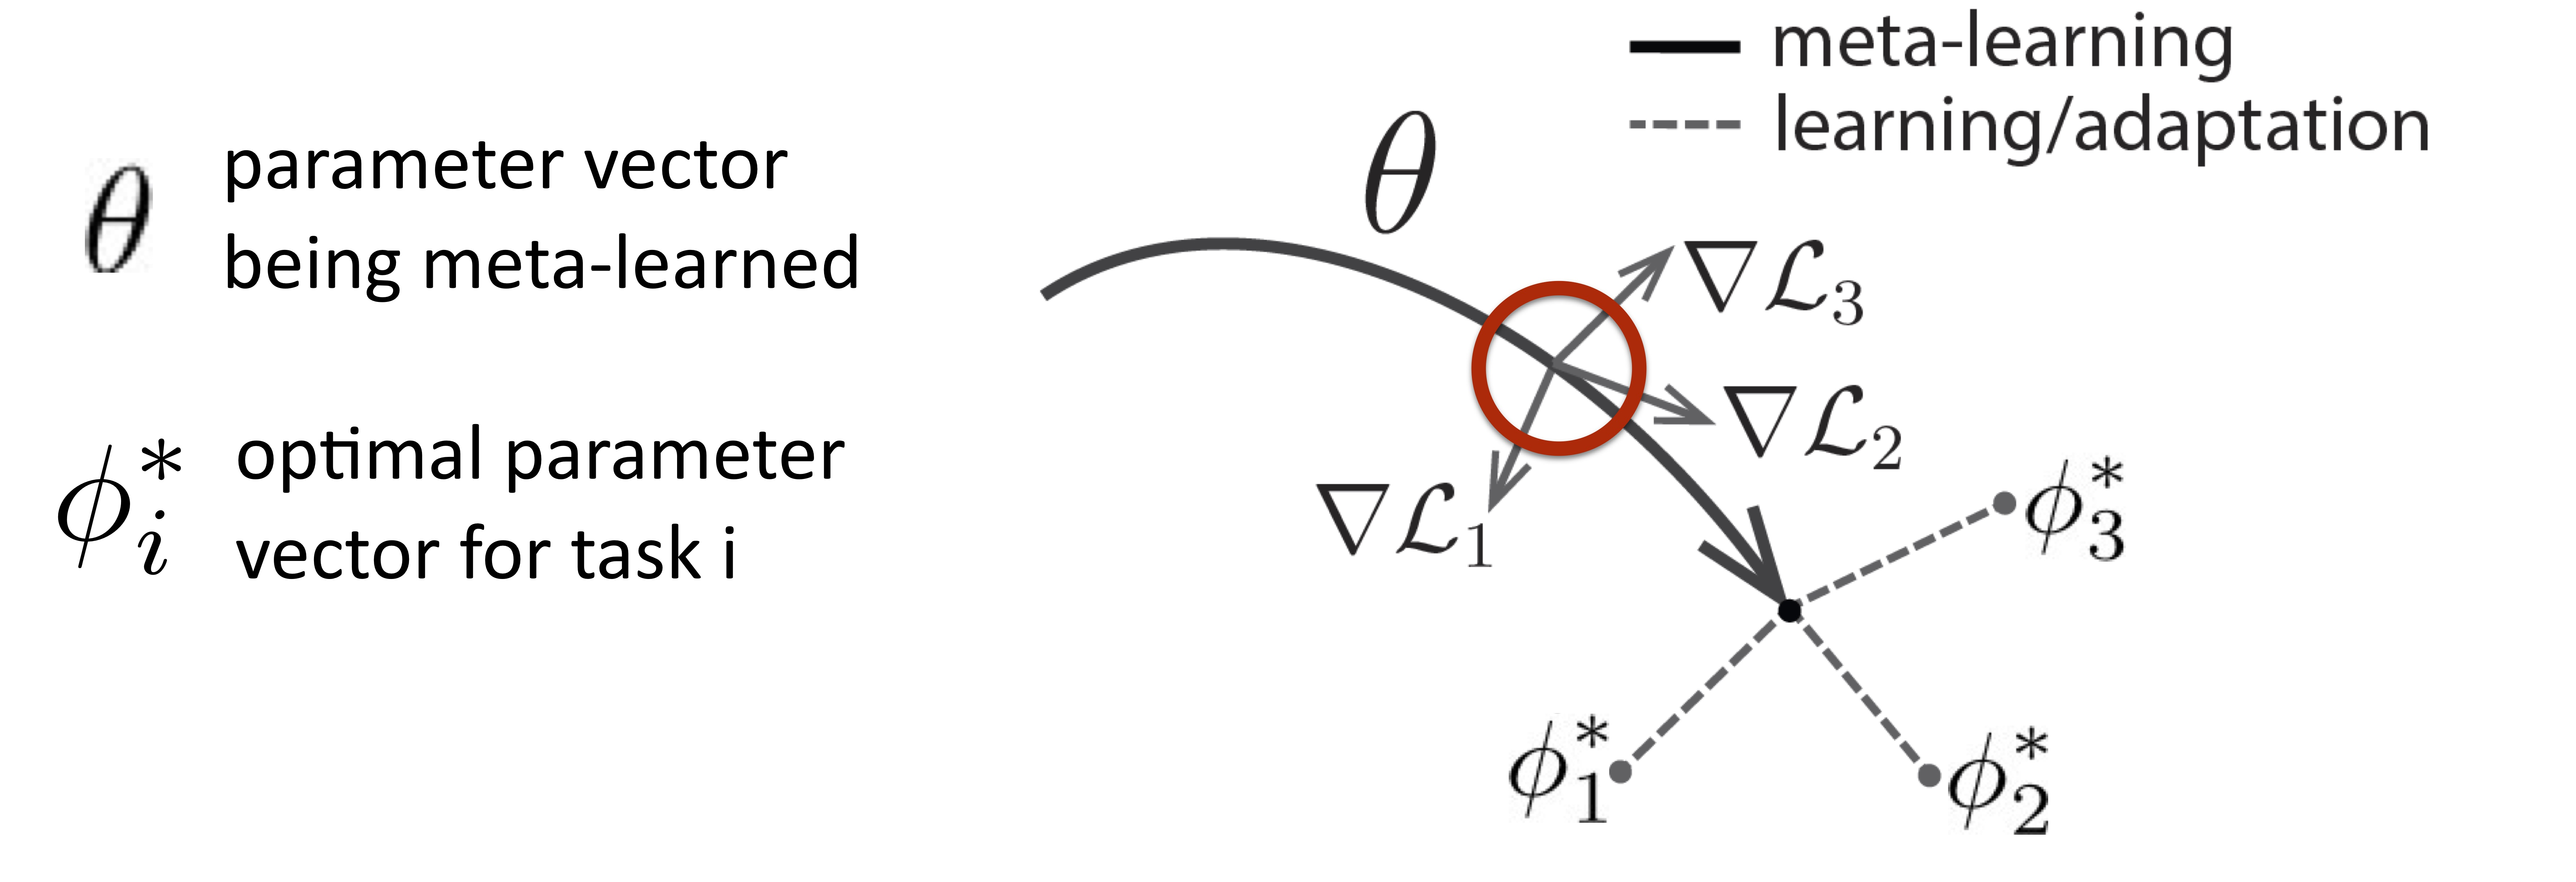
\includegraphics[width=0.65\textwidth]{images/maml.JPG}
    \caption{Model-Agnostic Meta-Learning}
    \label{fig:maml}
\end{figure}


{\bf Experiments;} Compare MAML with black-box approaches (SMAIL, MetaNetworks). Tend to find higher performance in domain adaption/extrapolated tasks. \\
$\ra$ Task was to shear digits in the Omnioglot dataset by some degree and inspect decay on performance. MAML rarely decays in performance. \\

Q: Does this learned structure come at a cost? \\

A: Not really! MAML function can approximation any function of $D_i^{\tx{train}}$, $x^{\tx{test}}$. Assumptions: nonzero $\alpha$, loss function does not lose information about the label, datapoints in $D_i^{\tx{train}}$ are unique. \\

$\therefore$ MAML has benefit of inductive bias without losing expressive power. \\

Another approach: probabilistic interpretation of optimization-based inference. Find: MAML is a form of {\it implicit} prior, roughly gradient-descent + early stopping, comes out to an implicit Gaussian prior. \\

Q; Other forms of priors expressible in meta-learning?  \\

A: Sure! Bayesian linear regression on learned features, or closed-form/convex optimization (as in ridge or logistic regression). \\


{\bf Challenges}:
\begin{itemize}
\item How do we choose an architecture that is effective for inner gradient step?
$\ra$ But, can do progressive neural search (w/ MAML) to overcome this.

\item Second-order meta-optimization can exhibit instabilities.
$\ra$ Lots of solutions available: 1) optimize only inner subset, 2) decouple learning rate, 3) introduce context variables, and so on
\end{itemize}


Approach 3: Non-parametric methods. In low data-regimes, non-parametric methods are simple and tend to work well. \\

$\ra$ During meta-test time: few shot learning $\equiv$ low data regime. During meta-training, still want to be parametric. \\

Q: Can we use parametric meta-learners that produce effectiv non-parametric learners? \\

A: Yes! Use non-parametric learners by comparing test data with training images. \\

Key Idea: learn a metric space that leads to more effective comparisons and predictions at test time. \\

%{\bf Comparison:} Compare these three approaches to meta-learning. 
{\bf Takeaways:} Each approach has some advantages/disavantages, listed in Figure~\ref{fig;maml_types}.
\begin{figure}[h!]
\centering
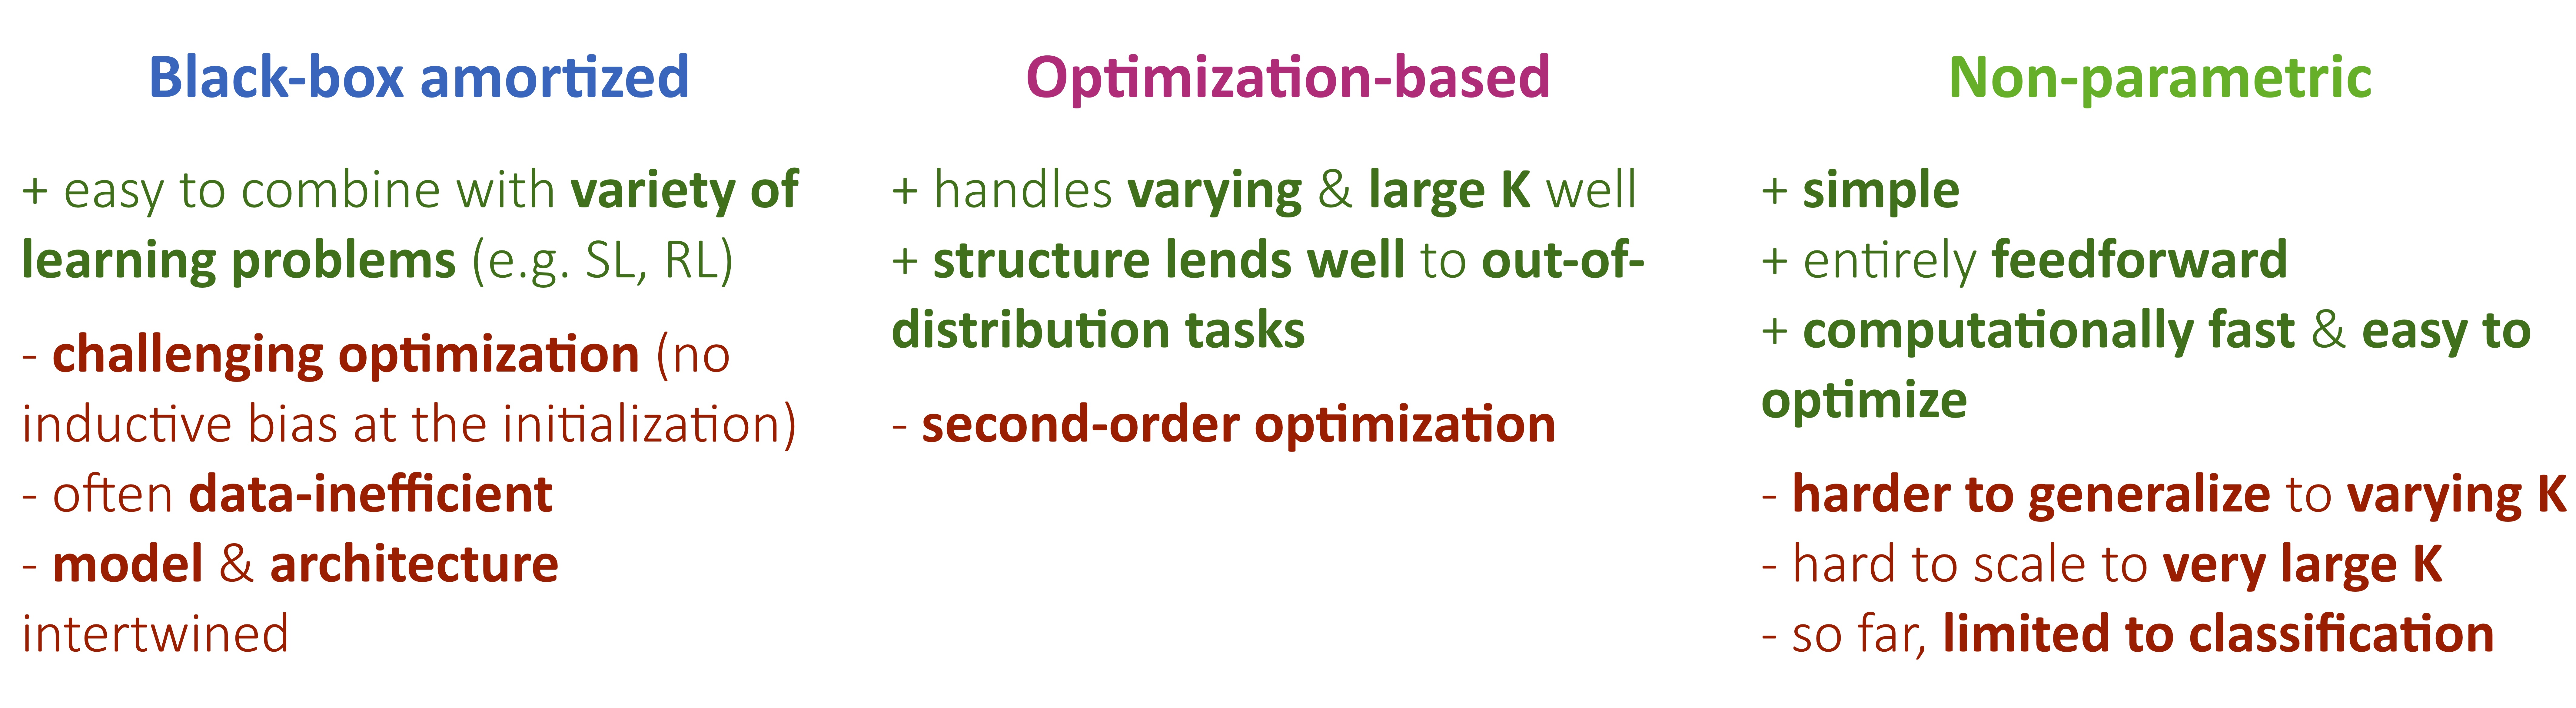
\includegraphics[width=0.85\textwidth]{images/maml_types.JPG}
\caption{Advantages and disadvantages of different approaches to meta-learning.}
\label{fig:maml_types}
\end{figure}


Approach 4: Bayesian Meta-Learning. \\

Assume we have a parameter prior $\Pr(\theta)$, $\Pr(\phi_i)$, can we sample $\phi_i \sim \Pr(\phi_i \mid x_i^{\tx{train}}, y_i^{\tx{train}})$. \\

Simple Idea: use neural net to produce a gaussian distribution over $h$, with $h$ some subset of relevant weights of the network (like the last layer). \\


Q: Okay, but what about Bayesian optimization-based meta-learning? \\

A: Sure! Lots of ways to do this. One idea is to model $\Pr(\phi_i \mid \theta)$ as Gaussian, perform variational inference for training (see Ravi and Beatson 2019). Another approach: do gradient-based inference on last layer only, use SVGD to avoid Gaussian modeling assumption (see work by~\citet{liu2016stein}). \\

$\ra$ Key Idea; Approximate $\Pr(\phi_i \mid \theta, x_i^{\tx{train}}, y_i^{\tx{train}})$ with a MAP inference. Very crude, but very convenient! \\


Further reading; ~\citet{garnelo2018conditional},~\citet{kim2018bayesian},~\citet{ravi2018amortized}.


{\bf Applications:}
\begin{itemize}
\item Vision: Few-shot image generation, image-to-image translation, generation of novel viewpoints.
\item Imitation Learning/RL: one-shot inverse RL, optimization based inference given demonstrations.
\item Language: Adapting to new programs, adapting to new languages, adapting dialogue agents to new personas.
\end{itemize}

\subsubsection{Meta-Reinforcement Learning}

Q: Why expect Meta-RL to be useful? \\

A: Well, major challenges in RL! Almost all related to the sample inefficiency of existing methods. Something TRPO, applied to a real robot, would take on the order of days or weeks for a robot to begin to make any kind of progress (in learning to walk). First, some background;\\

\ddef{Markov Decision Process (MDP)}{An MDP is a four tuple: $\langle, \mc{S}, \mc{A}, R, P\rangle$, with $\mc{S}$ a set of states, $\mc{A}$ is an action set, $P : \mc{S} \times \mc{A} \ra \Pr(\mc{S})$ denotes the transition function, and $R : \mc{S} \times \mc{A} \times \mc{S} \ra \mathbb{R}$ denotes the reward function.}

The goal is for an agent to learn a policy $\pi : \mc{S} \ra \mc{A}$ that maximizes long term expected reward:
\begin{align}
\theta^* = \argmax_\theta \bE_{\pi_\theta}\left[ R(\tau \mid \pi_\theta)\right],
\end{align}
where $\tau$ is the trajectory taken by $\pi_\theta$, and $R(\tau \mid \pi_\theta)$ picks out the rewards achieved by $\pi_\theta$. \\

``Every RL algorithm in a nutshell": finds $\pi_\theta$ either by: 1) learning a good policy directly, 2) learning a value function, or 3) learning a model and using it to find a good policy. \\

Meta-Learning so far: Learn $\theta$ uch that $\phi_i = f_\theta(D_i^{\tx{train}})$ is good for the test $D_i^{\tx{test}}$. \\

So, meta-RL problem is as follows;
\ddef{Meta-RL}{The Meta-Learning problem with the RL objective. That is, learn $\theta^*$:
\[
\theta^* = \argmax_{\theta} \nsum \bE_{\pi_{\phi_i}}\left[R(\tau \mid \pi_{\phi_i})\right],
\]
where $\phi_i = f_\theta(M_i)$}

Q: So how do we produce $M_i$, the meta-training MDPs? \\
A: One idea is to just choose related tasks (imagine we want a household chore robot, define $M_i$'s to be small and easy related tasks \\

Now, some meta-RL algorithms: similarly to supervised meta-learning, we also get a meta-RL based on black box approaches (here called ``recurrent policies"). \\

Main Question: how do we implement $f_\theta(M_i)$, with $M_i$ an MDP? Well, what should $f_\theta(M_i)$ do? \\

A: A few things: 1) improve policy with experience from $M_i$, and 2) Choose how to interact (that is, meta-RL must choose how to explore). \\

$\ra$ This mostly amounts to just running meta-RL with an RNN. \\

Q: But how do meta-RL algorithms explore effectively? This basically happens for free in this setting: optimizing reward over all episodes used in training leads to good exploration. \dnote{I don't see this, personally. Need to read more!} \\

{\bf Next View:} Treat meta-RL as an optimization problem. Standard RL formulate this as a policy gradient problem;
\[
\theta^* = \argmax_\theta \underbrace{\bE \left[R(\tau)\right]}{J(\theta)},
\]
then:
\[
\theta^{k+1} \la \theta_k + \alpha \nabla_{\theta_k} J(\theta)
\]


Next approach: meta-RL for partially observable RL! Need a richer environmental model:
\ddef{Partially Observable MDP (POMDP)}{A POMDP is a six tuple: $\langle S, A, O, P, E, r \rangle$, that is effectively an MDP, but the function $E$ generates observations from $O$ based on the current state. The agent only gets to perceive observations $o \in O$, not state.}

That is, the agent doesn't get to see everything relevant about the world, just some observation $o$ generated based on the state. \\

{\bf Key Idea:} Solving POMDPs is very hard! But, it's similar to meta-learning. Look for a policy $\pi_\theta(a \mid s, z)$, where we don't know $s$, only $z$. Works as follows: 1) Sample $z \sim \hat{p}(z_t \mid s_{1:t}, a_{1:t}, r_{1:t})$, 2) Act according to $\pi_\theta \mid s, z)$, acting as though $z$ was correct. \\


Three perspectives on Meta-RL:
\begin{enumerate}
\item Just RNN it: conceptually simple and easy, but vulnerable to overfitting and challenging to optimize.
\item MAML approach: good extraploating but complex (requires many samples).
\item POMDP approach: simple and effective, but also vulnerable to meta-overfitting.
\end{enumerate}

But: they're not that different! The POMDP approach is really just the RNN approach with an extra hidden variable, and the MAML approach is just a particular choice for the design of $f_\theta$. \\

\subsubsection{Challenges and Frontiers in Meat Learning}

Lots of exciting directions forward, but lots of challenges, too. \\

{\bf Challenge 1:} Meta-overfitting---meta learning requires a task distribution. Some approaches to meta-learning can {\it overfit} to these task distributions.\\

{\bf Challenge 2:} Task design---often these task distributions have to be chosen by hand, or are not diverse enough to encourage the right kind of behavior. It's hard to pick the task distribution in the right way! \\

{\bf Challenge 3:} Understanding which {\it algorithms} overfit---many difference approaches (black-box, optimization-based, non-parametric), but we don't have a sense of which kinds of algorithms are most vulnerable to meta-overfitting. \\

Q: What else can we do with meta-learning? \\

A1: Well, we might automatically propose tasks that generate the appropriate task distributions. $\implies$ ``Unsupervised meta learning", which refers to algorithms that learn to solve tasks efficiently without using hand-specified task distributions or labels during meta-training. \\

{\bf Challenge 4:} Memorization! Some algorithms may end up just memorizing solutions to the relevant test tasks.

{\bf Challenge 5:} How do we determine which task information should be in the input vs in the data? Broad task distributions can be useful, but makes exploration hard. If their too narrow, not representative enough. \\


\dnote{Had to run for the day!}

\spacerule



% ------------
% -- Monday --
% ------------
\newpage
\section{Tuesday June 11th: Main Conference}
I arrived today for the best paper award talk.

\subsection{Best Paper Talk: Challenging Assumptions in Learning Disentangled Representations}

Talk by Francesco Olivier Bachem. \\

\dbox{{\bf Central Question:} Can we learn disentangled representations in a purely unsupervised way?}


{\bf Context:} Representation learning. Consider a picture of a landscape. Goal of representation learning is to learn a function $f : \mc{X} \ra \Phi$, that translates each item of interest (say, images), into a set of features that capture the important characteristics about the images. \\

Q: What might we want to have in a representation?\\

A: lots of things! One idea, though: {\it disentanglement}. \\

\ddef{Disentanglement}{A single change in a factor should lead to single change in representation.}

Example: Consider geometric shapes placed in a scene, each of a different color/shape/size. If we vary one key aspect (a square's color or size, for instance) of the original image, the representation should change in exactly one way, too. \\

{\bf Focus:} Unsupervised learning od distentangle representations (so, critically, don't get to observe the ground truth factors of variation). \\

\dbox{Contributions:
\begin{enumerate}
    \item {\it Theoretical result:} for arbitrary data, unsupervised learning of disentangled representations is impossible.
    \item {\it Large-Scale Experimental Study:} Can we learn disentangled representations without looking at the labels?
    
    $\ra$ Can reconcile and still be effective! The theorem is about {\it worst case} data. Our data likely has the right structure that we can still learn these disentangled representations.
\end{enumerate}}

{\bf Experiments:} six methods, seven datasets, six metrics, yielding 10,000 trained models and 150,000 scores. \\

$\ra$ Questions to focus on:
\begin{enumerate}[Q1]
    \item Which method should be used?
    \item How do we choose the hyperparameters?
    \item How to select the best model from a set of trained models?
\end{enumerate}

Experimental findings:
\begin{enumerate}
    \item (Toward answering Q1): Random seed and hyperparameters seem to matter more than the choice of the objective function.
    \item (Toward answering Q2): Can't identify obvious trends that can be used as a rule-of-thumb for hyperparameter selection (but, transferring across tasks seems to help).
    $\ra$ Transfer of hyperparameters to different data set and metric does not seem to substantially
    \item (Toward answering Q3):  Unsupervisd model selection remains a key challenge!
\end{enumerate}

$\ra$ Implication: good runs from bad hyperparameter settings can easily outperform bad runs from good hyperparameter settings. \\

{\bf Key Takeaways:}
\begin{itemize}
    \item Role of inductive biases and supervision should be made explicit
    \item Concrete practical benefits of disentanglement should be demonstrated
    \item Sound, reproducible experimental setup with several data sets is crucial.
    \item Code: \url{github.com/google-research/disentanglement_lib/}. Also released 10,000 pretrained models.
\end{itemize}


\spacerule


\subsection{Contributed Talks: Deep RL}

Next we have 5 minute contributed talks. They're very short so I suspect I'll have a harder time transcribing.

\subsubsection{DQN and Time Discretization}

The speaker is Corentin Tallec. \\

{\bf Point:} Time discretization actually matters in deep RL! \\

$\ra$ Usual RL algorithms with high framerate leads to failure. Scalability often limited by algorithms; better hardware, sensers, actuators, can lead to new hyperparameters. \\

Q: Why is near continuous Q-learning failing? \\

A: As $\delta_t$ (time discretization), $Q^\pi(s,a) \ra V^\pi(s)$. As a result, at the limit, $Q$ no longer depends on actions! So we can't perform policy improvement. \\

Q: Can we solve this? \\

A: Yes! Can look at all these quantities, form new algorithms (for more, see the paper!). 

\spacerule

\subsubsection{Nonlinear Distributional Gradient TD Learning}

The speaker is Chao Qu. \\
 
{\bf Background:} Distributional RL considers stochastic nature of long term return, $Z(s,a)$. \\

{\bf This Work:} Consider a distributional counterpart of Gradient TD Learning. Properties:
\begin{itemize}
    \item Converges in off policy
    \item Converges with non-linear function approximation.
\end{itemize}

$\ra$ New algorithm: Distributionl GTD2. Uses temporal distribution difference instead of the temporal difference from GTD2. 

\begin{theorem}
Under mild assumptions, Distributional GTD2 converges in the limit.
\end{theorem}

{\bf Experiments:} Show that D-GTD2 does in fact converge.

\spacerule

\subsubsection{Composing Entropic Policies using Divergence Correction}

Talk by Jonathun Hunt. \\

Q: How do people solve complex motor control tasks such as juggling and unicycling at the same time? \\

A: Well, perhaps we tend to learn each of them independently, and then merging them together. \\

{\bf Note:} not option like! We don't do A then B, we do a new $A \circ B$ task. \\

{\bf Problem:} Given training tasks $T_1$ and $T_2$, we want to solve some merged task $T_b = T_1 + T_2$. \\

Prior work: generalized policy improvement~\cite{barreto} \dnote{CITE}, and compositional optimism (Haarnoja 2018 \dnote{CITE}). \\

Adapt existing ideas to this transfer setting:
\begin{enumerate}
    \item Successor Features
    \item Generalized Policy Improvement
    \item Divergence correction
\end{enumerate}

$\ra$ New algorithm for composing tasks in continuous action spaces. \\

\spacerule

\subsubsection{TibGM: A Graphical Model Approach for RL}

The speaker is Tameem Adel. \\

{\bf Genesis:} Graphical modeling approach for 1) increasing transferability generalization, and 2) adopt precise objectives and clear interpretations. \\

$\ra$ Do this by proposing an information theoretic objective aiming at maximizing ``local" reward and a more global measure (related to transfer). \\

{\bf Contributions:}
\begin{itemize}
    \item A graphical model based on
    \item Prove a correspondence between new objective and typical reward maximization objective.
    \item An information theoretic pretraining procedure focusing on exploration.
    \item State of the art results on 16 benchmark tasks.
\end{itemize}

\spacerule

\subsubsection{Multi-Agent Adversarial IRL}

The talk is by Lantao Yu. \\

{\bf Motivation:} Performance of RL agent relies on quality of reward function. \\

$\ra$ But, it can be hard to design the right reward function! \\

One solution: learn a reward function from expert demonstrations (as in imitation learning). \\

Q: But why shoul we care about reward learning? \\

A: Well, some advantages: 1) scientific inquiry (understanding animal behavior), 2) reward function is the most succinct, robust, and transferable description of a task, 3) can be helpful if we want to reoptimize policies in new environments.  \\

$\ra$ These properties are even more desirable in multi-agent setting! \\

\ddef{Single-agent IRL}{Find a reward function that explains expert behavior}

But: intractable! Too many reward functions explain the same behavior. \\

Generalize this setting to multi-agent using Markov Games:

\ddef{Markov Game}{A multi-agent generalization of MDPs~\cite{littman1994markov}}

Solution concept to a Markov Game is a Nash Equilibrium:
\ddef{Nash Equilibrium}{When no agent can achieve higher expected reward by changing its own policy.}

Method: introduced Logistic Stochastic Best Response Equilibrium (LSBRE). Optimize the pseudolikelihood objective. \\

{\bf Experiments:} Policy imitation performance. New method achieves state of the art in both cooperative/communicative and competitive tasks. \\

{\bf Summary:} New solution concept for Markov games, gives rise to new measures of interest. Propose the first multi-agent MaxEnt IRL framework.

\spacerule

\subsubsection{Policy Consolidation for Continual RL}

{\bf Motivation:} Catastrophic forgetting in neural nets! Nets tend to forget information from prior tasks. \\

$\ra$ Even happens in RL during continual learning, since distribution of seen states change over time as exploration/policy changes. \\

Agents should cope with: dicsrete and continuous changes to data distribution! \\

{\bf Contribiution:} Policy Consolidation agent. A bunch of agents are trained (via PPO) and connected via a KL distillation loss. \\

$\ra$ Final policy stored is the result of distilling all other policies trained. Ensures it doesn't deviate too much from prior performance. \\

{\bf Experiments:} Alternating task to explore effect of forgetting. Find their algorithm outperforms all other variants of PPO. \\

{\bf Future Work:} 1) Look at how to prioritize important memories during training, and 2) Adapt for off-policy learning. \\

\subsubsection{Off Policy Evaluation Deep RL w/o Exploration}

Consider: same off-policy algorithm (DDPG) used on same dataset with two differen approaches (orange and blue). \\

Agents: 1) Orange---interacts with the environment (standard rl loop), 2) Blue---just uses data from environment but doesn't actually interact! Yet, their performance is different \\

Q: Why would these be any different? \\

A: Extrapolation error: $Q(s,a,) \la r = \gamma Q(s',a')$, where $(s,a,r,s')$ come from the dataset. Basically, you might have a bad target $Q(s',a')$.\\

\ddef{Extrapolation error}{Attempting to evaluate $\pi$ without sufficient acccess to the $(s,a)$ pairs $\pi$ visits.}

Solution: batch-constrainted RL: only choose $\pi$ so that it selects $(s,a)$ pairs that are  in the dataset and maximizes performance. \\

$\ra$ New algorithm: Batch-constrained Deep Q Learning (BCQ). \\
\begin{enumerate}
    \item Imitate dataset via generative model
    \item $\pi(s) = \argmax_a Q(s,a)$
    \item Throw in some extra magic
\end{enumerate}

Finds that BCQ greatly outperforms some existing methods (DDPG), and is quite stable. \\

\spacerule

\subsubsection{Random Expert Distillation}

Talk by Ruohan Wang \\

\ddef{Imitation Learning}{Policy learning from a limited set of expert demonstrations}

Useful because: intuitive and efficient skill transfer, and can capture style/preferences of individual demonstrators. \\

$\ra$ Recent framework for IRL: Generative Adversarial Imitation Learning (GAIL). \\

But, optimization challenges; 1) training instability, and 2) sample inefficiency. \\

{\bf Main Contribution:} Random Expert Distillation (RED). Framework fir imitation learning using the estimated support of the expert policy as reward. \\

Optimize a new trajectory based loss based on a new reward function, and prove it approximates the right thing in the limit. \\

{\bf Experiment 1:} In MuJoCo, find high training stability and good sample efficiency compared to other approaches like GAIL. \\

{\bf Experiment 2:} Autonomous driving tasks with human actions as training data. Agent learns to follow the preferences of the trainer (speed, lane preference, and so on).

\spacerule

\subsubsection{Revisiting the Softmax Bellman Operator}

The speaker is Zhao Song. \\

Recall that the Bellman Operator is a contraction. \\

$\ra$ Mellowmax operator~\cite{asadi}\dnote{CITE} is also a contraction:
\[
max_{a'} Q(s',a') \ra \sum_{a'} \frac{\exp \tau Q}{\sum_b \exp \tau Q(s',b)}
\]
Q: Is softmax really as bad as sour milk? (credit to Ron Parr). \\

{\bf Idea:} combing the max function in the target network of DDQN with softmax. \\

$\ra$ Gives rise to the SQDN, achieves higher scores than DQN on most Atari games. \\

Thus: analysis of softmax is warranted! \\

\begin{theorem}
Analysis showing: good performance, guaranteed convergence, smaller error, reduction bound, and overestimation error monotically increases w.r.t. $\tau$ (inverse temperature).
\end{theorem}

\spacerule
\subsection{Contributed Talks: RL Theory}

More RL!

\subsubsection{Distributional RL for Efficient Exploration}

Talk by Hengshuai Yao. \\

{\bf Point:} Lots of sources of uncertainty in RL---estimation (in finite data regime), but also other factors like environmental stochasticity, opponents' play in game, and so on. \\

$\ra$ Exploration strategy based on uncertainty: {\it optimism under uncertainty}. In multi-armed bandits, choose arm according to:
\[
a = \argmax_k \hat{\mu}_k + c_k,
\]
where $\hat{\mu}_k$ is estimated mean payoff, and $c_k$ is some measure of uncertainty in this estimate (UCB like). \\

But! Using naive exploration bonus doesn't always work: favors actions with high intrinsic uncertainty forever. \\

{\bf New Idea:} To use optimism in face of uncertainty, perform decaying schedule of the weight of uncertainty. This ensures that as more evidence is gathered, the agent starts to exploit more.
\spacerule

\subsubsection{Optimistic Policy Optimization via Importance Sampling}

Talk by Matteo Papini. \\

{\bf Problem:} Policy Optimization.
\begin{itemize}
    \item Parameter space $\Theta \subseteq \mathbb{R}^d$
    \item Parapmetric policy for each $\theta \in \Theta$
    \item Each policy induces a distr. over trajectories, with $R(\tau)$ the return of the trajectory.
    \item Goal is to find he parameters that maximize the expected return:
    \[
    \max_{\theta \in \Theta} \bE[R(p_\tau \mid \theta)].
    \]
\end{itemize}

Challenge, though: exploration here is hard! \\

Q: What if we think about this as a multi-armed bandit? \\
Then:
\begin{itemize}
    \item Arms: parameters $\theta$
    \item Payoff: expected return $J(\theta)$
    \item Continuous Multi-Armed Bandit, effectively.
    \item Take advantage of arm correlation through trajectory distributions.
    \item Use Important Sampling to update return of a candidate policy.
\end{itemize}

{\bf Main result:} new algorithm ``\textsc{Optimist}", enjoys sublinear regret:
\[
Regret(T) - \tilde{O}(\sqrt{dT}).
\]

Code: \url{github.com/wolfLo/optimist} 

\spacerule

\subsubsection{Neural Logic RL}

The talk is by Shan Luo. \\

Two main challenges of deep RL: 1) How can we generalize learned policies from one task to another?, and 2) How can we interpret these learned policies? \\

{\bf Approach:} use background knowledge to learn concepts and relations, like \texttt{grandfather(x,y)}. To do so, use {\it differentiable inductive logic programming}.

$\ra$ Idea: learn logic rules with policy gradient (a new architecture, DILP, trained with REINFORCE). \\

{\bf Experiments:} For many settings, achieve high reward compared to MLP agent (baseline). \\

\spacerule

\subsubsection{Learning to Collaborate in MDPs}

The talk is by Goran Radanovic. \\

{\bf Motivation:} Human-AI collaboration---consider a helper AI assisting a person in solving some task. \\

$\ra$ The agents might share a common goal, but view the different in some way, or have different behavioral differences. \\

Formal model: two-agent MDP, where agents have {\it commitments}. \\

$\ra$ Goal is to design a learning algorithm (for the first, non-human AI) that achieves sublinear regret. \\

Challenge: from the perspective of A1, the world looks like a non-stationary MDP due to the presence of A2 (the person). \\

{\bf Main Contribution:} Experts with Double Recency Bias, a new algorithm for this setting, based on the recency bias. 

\begin{theorem}
(Main Result): The regret of this algorithm decays as $O\left(T^{\frac{1}{4}}\right)$.
\end{theorem}

\spacerule

\subsubsection{Predictor-Corrector Policy Optimization}

Talk by Ching-An Cheng. \\

{\bf Problem:} Episodic policy optimization. So, agent is trying to optimize some policy $\pi(a \mid s)$, that achieves high return. \\

$\ra$ One goal: sample efficiency. We should spend time on planning/thinking before any real interactions. \\

Q: Why should we use models? \\

A: Can summarize past experience, can be more sample-efficient, and can optimize a policy efficiently without real world interactions. \\

Q: Why don't use models? \\

A: Well, models are always inexact! Weaknesses of model can be exploited in policy optimization. \\

Q: Can we reconcile these two camps? \\

A: Sure! This paper: PicColo (see talk title). A meta algorithm based on the idea that: ``shoud not fully trust a model but leverage only the correct part" \\

$\ra$ How can this be achieved?
\begin{itemize}
    \item Frame policy optimization as predictable online learning (POLL
    \item Design a reduction based algorithm for POL to reuse known algorithms.
    \item When translated back this gives a meta-algorithm for policy optimization.
\end{itemize}

Online learning: consider a learner and an opponent, with the learning chooses a decision $\pi_n \in \Pi$ every so often. Opponent chooses a loss function to minimize performance, rinse and repeat. \\

$\ra$ Most common performance measure is {\it regret}. {\bf Idea:} Define policy optimization as an online learning process. \\

$\ra$ Algorithmically: can try typical no-regret algorithms (mirror descent), but not optimal! Want to learn faster. \\

Idea: view predictability as the ability to predict future gradients. Introduce the following model:

\ddef{Predictive model}{A function that estimates the {\it gradient of future loss}
\[
\Phi_n(\pi) \approx \nabla \ell_n(\pi)
\]}

Now, develop an algorithm based on this predictability model. \\

$\ra$ Want a reduction from predictability to online learning. This is PicColo! \\

Suppose we have a predictable learning problem, idea is to turn it into an adversarial one. So:
\[
\ell_n(\cdot) = \hat{\ell}_n(\cdot) + \Delta_n(\cdot),
\]
which is a combination of prediction loss (the first term) and error (the second loss). \dnote{I didn't catch what the second source of error is}

PicColO: two steps---1) Prediction step ($\pi_n = \hat{\pi}_n - \eta_{n}\hat{g}_n$, and 2) correction step---$\hat{\pi}_{n+1} = \eta_n(g_n - \hat{g}_n$, with $g$ the return.\\

{\bf Experiments:} Compare PiColo with a variety of other algorithms on MuJoCo tasks. \\

{\bf Summary:}
\begin{itemize}
    \item PicColO can change a model-free algorithm to be faster but without the bias.
    \item Predictive model can be viewed as a unified interface for injecting prior
    \item As PicCoLO is degiend for general predictable online learning, we expect applications to other problems and domains.
\end{itemize}


\spacerule

\subsubsection{Learning a Prior over Intent via Meta IRL}

Talk by Kelvin Xu. \\

{\bf Motivation:} we often assume we have a well specified reward function! \\

Q: How can an agent infer rewards from one or a few demonstrations? \\

$\ra$ This work! Use demonstrations from previous tasks to induce tasks priors that can be used in new tasks. \\

{\bf Main idea:} use prior task information to accelerate inverse RL. \\

$\ra$ Builds on MAML (see meta-learning tutorial!). \\

{\bf Experiment:} Sprite world environment, and 2) First person navigation task. In both cases, learn task priors from meta-training task, use to learn quickly in test tasks. \\

$\ra$ Results: performs very well even only given a small number of demonstrations. \\

\spacerule

\subsubsection{DeepMDP: Learning Late Space Models for RL}

Talk by Carles Gelada. \\

{\bf Goal:} Find simple representations for RL. \\

Approach: learn a latent space model $\bar{M} = \langlage \bar{\mc{S}}, \bar{\mc{A}}, \bar{R}, \bar{T} \rangle$. Based on two losses;
\begin{align}
    &\bar{R}(s,a) \approx R(s,a), \forall_{s,a} \\
    \bar{T}(s' \mid s,a) \approx T(s' \mid s,a), \forall_{s,a,s'}.
\end{align}

Using these losses, ensure that $\phi$ is a good representation in the sense that it only throws out bad/useless policies. \\

{\bf Experiments 1:} Donut world. Image of a circle. Embedding function ends up finding a similar representation. \\

{\bf Experiments 2:} Atari w/ C51, find improvement over baselines.

\spacerule

\subsubsection{Importance Sampling Policy Evaluation}

Talk by Josiah Hanna. \\

Note: lots of recent empirical RL success! \\

But: for RL to be successful, we must ask: ``How can RL agents get the most from small amounts of experience?". \\

{\bf Core Contribution:} Study important sampling for the RL sub-problem of policy evaluation. More specifically: replace the denominator of importance sampling with an estimate, and prove that this is justified empirically and theoretically. \\

Typical importance sampling in RL:
\[
OIS(\pi, D) = \frac{1}{m} \nsum \Pi_{t=0}^L \frac{\pi(a_t \mid s_t)}{\pi_D(a_t \mid s_t} \sum_{t=0}^L \gamma^t R_t
\]
They replace the denominator with an MLE {\it estimate} of the behavioral policy's performance:
\[
New-IS(\pi, D) = \frac{1}{m} \nsum \Pi_{t=0}^L \frac{\pi(a_t \mid s_t)}{\hat{\pi}_D(a_t \mid s_t} \sum_{t=0}^L \gamma^t R_t
\]
Paper provides theory and experiments showing this is a good thing to do. 

\spacerule

\subsection{Learning from a Learner}

Talk by Alexis Jacq. \\

{\bf Goal:} Want to learn an optimal behaviour by watching others learning. \\

Assume: learning is optimizing a regularized objective:
\[
J(\pi) = \bE_\pi \left[ \sum_{t} \gamma^t(r(s_t,a_t) + \alpha H(\pi(\cdot \mid s_t))\right].
\]
The value of a state action couple is given by the fixed point of the regularized bellman equation. Moreover, the softmax is an improvement of the policy (see \citet{haarnoja2018soft}). \\

{\bf Experiments:} on MujoCo, find improvement.

\spacerule

\subsection{Separating Value Functions Across Time-Scales}

Talk by Joshua Romoff. \\

Multi-step returns:
\[
G_t^k = \sum_{i=0}^{k-1} \gamma^i r_{t+1} + \gamma^k V(s_{t+k}).
\]
Can choose $k$ to trade-off between bias-variance. Or, the $\lambda$ returns:
\[
G_t^\almbda := (1-\lambda) \sum_{k=1}^\infty \lambda^{k-1} G_t^k.
\]
Many tasks are {\it discounted:} when $\gamma \ra 1$, training $V_\gamma$ is difficult. \\

Q: Why use discount factor?\\

A: Well, it makes the problem simpler. Only ever thinking about the next few rewards, so agents can learn to make decisions more easily.\\

$\ra$ But, add a lot of bias! Sometimes we don't really care about early rewards more. \\

{\bf Take a step back:} what would the ideal RL agent do? It would learn to do well quickly! \\

Ideally: want to 1) learn with a discount factor that is large but, 2) built on top of methods that are computationally and sample efficient. \\

{\bf Solution:} define a sequence of $\lambda$s:
\[
\Delta ;= \{\gamma_0, \gamma_1, \ldots, \gamma_Z\},
\]
where $\gamma_i \leq \gamma_{i+1}, \forall_i$. \\

Then, form a sequence of Bellman Equations using this sequence of $\gamma$s:
\begin{align}
W_0 &: r_t + \gamma_0 W_0(s_{t+1}) \\
W_{i > 0} &: (\gamma_i - \gamma_{i-1})V_{\gamma_{i-1}}(s_{t+1}) + \gamma_i W_i(s_{t+1}).
\end{align}
Algorithm: TD$(\Delta)$, equivalent to standard $TD(\lambda)$. \\

Analysis: Under some conditions, equivalent to standard TD$(\lambda)$.
    
    $\ra$ So, why would you do this new, sequenced thing?
    
    $\ra$ Well, equivalent when using linear function approximation. And: 1) Same learning rates for each $W$, and 2) Same $k$-step, $\gamma$, and $\lambda$ for each $W$.
    
    $\ra$ (But of course, don't have to set these parameters the same way). \\
    
Can extend TD($\Delta$) to Deep RL: 1) Share network multiple outputs, 2) Train $W$s as described, 3) Use the same of $W$s instead of $V$s \\

{\bf Experiments:} Tested in Atari, contrast TD($\Delta)$ with PPO and PPO+ (PPO but with additional parameters). \\

$\ra$ Further explore what $TD(\Delta)$ learns by plotting the value function. \\

Things they didn't try (but we should!):
\begin{itemize}
    \item Adding {\it more} $W$s.
    \item Q-learning extension (everything they tried was on policy).
    \item Model architecture for the value functions: could explore using fewer parameters, and so on.
    \item Distributed variant.
\end{itemize}

{\bf Summary:}
\begin{enumerate}
    \item Deompose the value function based off of $\gamma$
    \item Train with Bellman-like equations
    \item Improves sample efficiency
\end{enumerate}

\spacerule
\subsubsection{Learning Action Representations in RL}

Talk by Yash Chandak. \\

{\bf Problem:} consider RL problems with {\it thousands} of possible actions! (applications might be a medical treatment, advertisement, or portfolio management). \\

$\ra$ Might capture this by learning options~\cite{sutton1999between}, but usually leads to learning {\it too many options}. \\

Q: How can we learn good action representations, but not learn too many? \\

{\bf Key Insights:}
\begin{enumerate}
    \item Actions are not independent discrete quantities
    \item There is a low dimensional structure underlying their behavior.
    \item This structure can be learned independent of the reward.
    
    \item Thus, instead of raw actions, agent can act in this new space of bejavior, behavior can be generalized to similar actions. 
\end{enumerate}

New Algorithm: 1) Supervised learning of action representations, and 2) Learn internal policy of these representations using policy gradient. \\

{\bf Experiments:} Applied algorithm to a variety of domains with rich action spaces (recommendation in photoshop, for instance), find consistently good performance. \\

\spacerule

\subsubsection{Bayesian Counterfactual Risk Minimization}

Talk by Ben London. \\

{\bf Problem:} Learning from Logged Data to recommend music. \\

Challenges:
\begin{enumerate}
    \item Feedback is bandit feedback, so only learn from chosen actions
    \item Data is biased based on chosen logging policy.
\end{enumerate}

$\ra$ One way to counteract this bias is to use inverse propensity scoring:
\[
\argmin_{\pi} \frac{1}{n} \nsum -r_i \frac{\pi(a_i \mid x_i)}{p_i}.
\]
Can also use {\it variance regularization}, giving rise to the Counterfactual Risk Minimization (CRM) principle;
\[
\argmin_{\pi} \frac{1}{n} \nsum -r_i \frac{\pi(a_i \mid x_i)}{p_i} + \lambda \sqrt{Var(\pi, S)}
\]
$\ra$ Motivated by PAC analysis, ensures low generalization error. \\

{\bf This Work:} Bayesian view of CRM (motivated by PAC-Bayes analysis). Yields a nice generalization error bound. \\

$\ra$ Application to mixed logits. \\

\spacerule

\subsubsection{Per-Decision Option Counting}

Talk by Anna Haratunyan. \\

{\bf Motivation:} Agents that reason over long temporal horizons. But: {\it horizon depends on choice of $\gamma$}. \\

Q: Perhaps we can do this with options~\cite{sutton1999between}? \\

A: But, doesn't really handle different horizons. \\

\dbox{{\bf Main contribution:} generalize the options framework to allow for per-option discounting.}

$\ra$ That is, add a per-decision option discount, $(\gamma_r, \gamma_p)$. \\

In this framework, they identify a bias-variance trade-off captured by these new discounts. \\

\spacerule

\subsubsection{Problem Dependent Regret Bounds in RL}

Talk by Andrea Zanette. \\

{\bf Focus:} Exploration in episodic, tabular RL. \\

$\ra$ State of the art regret bounds:
\begin{itemize}
    \item No intelligent exploration $\tilde{O}(T)$
    \item Efficient Expliration; $\tilde{O}(H\sqrt{SAT})$
    \item Lower Bound: $\tilde{O}(\sqrt{HSAT})$
    \item Below the Lower Bound: problem dependent!
\end{itemize}

Main result (requires variance of value, and scaling of reward)
\begin{theorem}
With high probability, can achieve regret of:
\[
\tilde{O}(\sqrt{\mathbb{Q}^*SAT}),
\]
where $\mathbb{Q}^*$ is a problem dependent term.
\end{theorem}

Answers an open conjecture from Jiang and Agarwal 2018 (COLT): any algorithm must suffer $H$ regret in goal-based MDPs. \\

$\ra$ Also explore effect of stochasticity on regret. \\

\spacerule

\subsubsection{A Theory of Regularized MDPs}

Talk by Matthieu Geist. \\

{\bf Motivation:} Many deep RL algorithms make use of regularization, but no general theory of how to regularize in RL. \\

$\ra$ This work: generalizes regularization in RL in two ways:
\begin{enumerate}
    \item Larger class of regularizers
    \item General modified policy iteration scheme.
\end{enumerate}

LEt $\Omega : \Delta_A \ra \mathbb{R}$ be a strongly convex function. The convex conjugate is a smoothed maximum:
\[
\forall_{q_s} \in \mathbb{R}^A, \Omega^*(q_s) = \max_{\pi_s \in \Delta_A} (\pi_s, q_s) - \Omega(\pi_s).
\]

Thus, we can regularize the Bellman Equation:
\begin{equation}
    T_{\pi,\Omega}[V] = T_\pi[V] - \Omega(V).
\end{equation}

The regularized Bellman Operators satisfy the same properties as the original ones: 1) $T_{\pi, \Omega}$ is affine, 2) Monotonicity, distributitivity, and $\gamma$-contraction. \\

$\ra$ Introduce a new algorithmic scheme, regularized policy improvement, and prove the following result:

\begin{theorem}
After $k$ iterations of reg-MPI, the loss is bounded.
\end{theorem}

$\ra$ Can also use this theory to characterize existing approaches to regularization in RL (like TRPO, DPP, and so on). \\

{\bf Summary:}
\begin{itemize}
    \item Bridges some gaps between dynamic programming and optimization
    \item Introduced temporal consistency equations, as with entropy
    \item Can generalized existing approaches to regularization, such as regularized policy gradient.
\end{itemize}


\spacerule

\subsubsection{Discovering Options for Exploration by Minimizing Cover Time}

\dnote{Now, our paper!} The talk is by Yuu Jinnai. \\

{\bf Goal:} Choose options that are effective for exploration. \\

Contribution:
\begin{enumerate}
    \item Introduce an objective function for exploration called {\it cover time} (see below).
    \item Algorithm for option discovery that minimizes an upper bound on the cover time.
    
    $\ra$ Computes the {\it Fiedler} vector based on the graph induced by the graph of the MDP, uses it to minimize the cover time.
\end{enumerate}

\ddef{Cover Time}{The expected number of steps needed to visit every state.}

\begin{theorem}
The upper bound on the cover time is improved;
\[
\bE[C(G')] \leq \frac{n^2 \ln n}{\lambda_2 C(G')}
\]
\end{theorem}

Performed empirical comparison contrasting learning performance with different kinds of options. \\

\spacerule

\subsubsection{Policy Certificates: Towards Accountable RL}
Talk by Cristoph Dann. \\

Key contribution: new algorithm for episodic tabular MDPs with:
\begin{theorem}
PAC Bound;
\[
\tilde{O}\left(\frac{SAH^2}{\eps^2}\right),
\]
and a matching regret bound.
\end{theorem}

Motivation, though: {\it accountability}, not necessarily sample efficiency. \\

Q: How good will my treatment be? Is it the best possible? \\
$\ra$ What kinds of methods can answer these kinds of questions? 

{\bf Main IDea:} Introduce {\it policy certificates} to add accountability.
\ddef{Policy Certificate}{Confidence interval around optimal and algorithm's performance}

$\ra$ Natural extension of model-based optimistic algorithms. \\

Challenge: $Q^\pi$ is random, so it can be hard to compute confidence intervals for it. But! From optimism, we know $Q^\pi \ra Q^*$ at a known rate. So, we can bound this quantity. \\

Two main benefits:
\begin{enumerate}
    \item More accountable algorithms through accurate policy certificates.
    \item Better exploration bonuses yield minimiax-optimal PAC and regret bounds.
\end{enumerate}

\spacerule

\subsubsection{Action Robust RL}


Talk by Chen Tessler. \\

{\bf Goal:} Achieve robustness in RL/MDPs. Consider cases of abrupt disruption, highly stochastic problems, and so on. \\

$\ra$ Thus, study robust MDPs where;
\[
\pi_\alpha(\pi, \pi^') = \begin{cases}
\pi& w.p. 1-\alpha \\
\pi^'& w.p. \alpha
\end{cases}
\]

Introduce an algorithm as a a player in a two player, adversarial game. Guaranteed to converge to nash. \\

$\ra$ Propose a Deep RL variant based on this robust MDP algorithm, experiment on MuJoCo. 

\spacerule

\subsubsection{The Value Function Polytope}

Talk by Robert Dadashi. \\

{\bf Central Question:} Can we characterize the geoemtry of the space of possible value functions for a given MDP? \\

Why ask this?
\begin{itemize}
    \item Relationship between policy space and value function space
    \item Better understand the dynamics of existing algorithms
    \item New formalism of representation learning in RL.
\end{itemize}

Main Result: what is the geometry of the space of value functions of a given MDP?
\begin{theorem}
The ensemble of value functions are (possibly non-convex) value polytopes.
\end{theorem}

Building blocks: 1) the line theorem (value functions of mixtures of similar policies describe a line in value function space), and 2) boundary theorem (\dnote{missed explanation}).\\

Ongoing future work: new representation learning schemes for RL, new actor-critic algorithms. \\

\dnote{And that's a wrap for Tuesday!}



% ------------
% -- Tuesday --
% ------------
\newpage
\section{Wednesday June 12th: Main Conference}
The day (afternoon, really) begins with contributed talks on multitask/lifelong learning.

\subsection{Contributed Talks: Multitask and Lifelong Learning}

Most talks will again be five minutes, with a few being 20. 

\subsubsection{Domain Agnostic Learning with Disentangled Representations~\cite{peng2019domain}}

Talk by Xingchao Peng. \\

{\bf Idea:} Carry out supervised learning when the domain shifts. \\
$\ra$ Well motivated by applications (lots of cases where training data differs from true task).

\ddef{Domain Adaptation}{Train on some source domain, $P_S(X_S,Y_S)$, with lots of labeled data, then test of target $P_T(X_T,Y_T)$.}

Example: Performing image recognition on canonical, full color images, then translating to recognition on {\it sketches}, some of which might be black and white. \\

Lots of related work~\cite{saito2018maximum,ganin2016domain,tzeng2017adversarial}. \\

{\bf New Approach:} Deep Adversarial Disentangled Autoencoder (DADA).
\begin{itemize}
    \item Class disentanglement: disentangle to class-irrelevant and domain-invariant features
    \item Domain disentanglement: Disentangle to domain-specific and domain invariant features.
\end{itemize}

Example: class-invariance vs. domain invariance.

$\ra$ Domain invariance; given two images, one from a real car, one of a painting of a car $\ra$ pass both into some neural net yields some features. In principle these features should be {\it domain-invariant} since they're found in both of these car renditions. \\

$\ra$ Class invariance: take a look at the backgrounds of the cars, this would yield the {\it class invariant} features, since they identify different classes. \\

Class disentanglement: train class identifier with the following loss:
\[
L_{ce} = \bE_{x,y} \left[\sum_{k=1}^K \indic\{k=y\} \log C(f_D)\right].
\]
Create a similar loss (and piece of the architecture) for domain disentanglement;
\[
L_{vae} = ||\hat{f}_G - f_G||^2 + \KL{q(z \mid f_g)}{p(z)}.
\]
{\bf Experiments:} Three benchmarks: 1) 5 digit datasets, 2) Office domains, 3) DomainNet, each of which contains a variety of domains and categories. \\

$\ra$ Finding: new model (DAD) improves performance over SOTA by 6\% on average across these datasets.

\spacerule


\subsubsection{Composing Value Functions in RL~\cite{van2019composing}}

Talk by Steve James. \\

\dbox{{\bf Central Question:} Can we blence value functions together from different tasks to solve interesting combinations of the tasks without further learning?}

In general, consider skills $Q_1$ and $Q_2$. Typically, we see $Q_1 \oplus Q_2 = \frownie$. \\

This work: considers entropy regularized RL:
\[
r_{ent}(r,s) = r(s,a) - r \KL{\pi_s}{\bar{\pi}_s}.
\]


With entropy regularized RL we show that: $Q_1 \oplus Q_2 = \smile$ \\

Idea: OR task composition: can optimally compose $Q(\square)$ and $Q(\circ)$ to solve the task of collecting $\square$ OR $\circ$. \\

Corollary: in the limit, prov that $Q(\circ OR \square) = \max\{Q(\circ), Q(\square)\}$. \\

{\bf Experiment:} Agents should pick up some object, train in tasks where they have to pick up just one type, then test in case where either is OK. \\

Summary:
\begin{enumerate}
    \item Can do zero shot composition to provably find solution to OR tasks.
    \item Works well in experiments!
\end{enumerate}

\spacerule
\subsubsection{CAVIA: Fast Context Adaptation via Meta Learning~\cite{zintgraf2019fast}}

Talk by Luisa Zintgraf. \\

{\bf Idea:} Meta-learning for fast adaptation---learn how to map $x$ to $y$ on new tasks, fast and with little data. \\

$\ra$ Earl approach: MAML (see meta-learning tutorial). \\

{\bf New Algorithm:} CAVIA: Fast Context Adaptation via Meta Learning--- 1) less prone to overfitting and 2) interpretable. \\

$\ra$ Many tasks and currrent benchmarks only require task identification. many parameters and few data points can lead to {\it overfitting}. \\

{\bf Experiment 1:} sine curve experiments. Task is defined by learning amplitude and phase. MAML require 1500 parameters, whereas CAVIA requires only 2 context parameters. \\

$\ra$ Context parameters are interpretable, and can be reused across tasks. \\

{\bf Experiment 2:} mini-imagenet experimnents. As the network becomes more complex, MAML requires 30000 parameters, hwereas cAVIA only requires a few hundred. \\

\spacerule

\subsubsection{Gradient Based Meta-Learning~\cite{khodak2019adaptive}}

Talk by Mikhail Khodak. \\

Q1: What kinds of task-relationships can meta-learning algorithms exploit?  \\

Q2: Are we restrictinv outsrleves by using such simple methods ? \\

Q3: How does meta-learning relate to classical multi-task methods? \\

{\bf This Work:} Address these questions in the convex case. Answers:

\begin{enumerate}
    \item Better avg. performance per-task if optimal task-parameters are close together
    \item GBML is the best we can do without stronger task-similarity assumptions
    \item NAtural connection between GBML to regularized multi-task learning
\end{enumerate}

Main strategy: connection to online convex optimization.\\
$\ra$ Consider what a standard gradient based method does. Pick first initialization $\phi_1 \in \Phi$, then for task $t = 1 \ldots T$;
\begin{enumerate}
    \item Run $m$ steps of SGD
    \item \dnote{Missed it.}
\end{enumerate}
Can then import guarantees from online convex optimization, specifically regret guarantees that encode distance from initialization. \\

Main result:
\begin{theorem}
GRBML achieve average regret of:
\[
O\left(D + \frac{\log T}{T} \sqrt{m}\right),
\]
where $T$ is the number of tasks, $D$ is the radius, \dnote{didn't catch $m$, presumably num samples}.
\end{theorem}

\spacerule

\subsubsection{Towards Understanding Knowledge Distillation~\cite{phuong2019towards}}

Talk by Mary Phuong. \\

{\bf Idea:} Knowledge distillation. A teacher (trained neural net), comes up with/represents a function $f_\theta : \mc{X} \ra \mc{Y}$. Then, would like to compress this function into a smaller/simpler network (a student!). \\

Q: How effective is distillation? Make this concrete by studying a quantity called the {\it transfer risk}, measuring how bad the distillation process can be. \\

Setting: linear distillation: 1) linear teacher, 2) student is a deep neural net. \\

{\bf Results:}
\begin{enumerate}
    \item Can compute exactly what the student will learn! Teacher is $f_t(x) = w^\top x$, then student will be either exactly the teacher (depending on amount of data).
    \item Can also bound the transfer risk:
    \begin{align}
        n_data &\geq d \implies risk = 0 \\
        n_data &< d \implies risk \leq \left(\frac{\log n_{data}}{n-data}\right)^\kappa, \\
    \end{align}
    with $\kappa \in [0,\In infty)$ the easiness of the distr.
\end{enumerate}

\spacerule

\subsubsection{Transferable Adversarial Training~\cite{liu2019transferable}}

Talk by Hong Liu. \\

{\bf Typical Assumption:} training data and test data are drawn from same distribution. \\

$\ra$ What if we change this? \\

$\therefore$ This work: how do we generalize a learner across different distributions $P$ and $Q$. \\

{\bf Goal:} bound the target error (on distr $Q$) with error from train error (on distr $P$). \\

$\ra$ existing theory based on domain adaptation. \\

Prior work (adversarial feature adaptation):
\begin{enumerate}
    \item Minimize source risk
    \item Minimize discrepancy term: learn a few feature representation where discrepancy is minimized
    \item Define as a two player game: domain discriminator tries to discriminate the source and target domain, while feature extractor tries to confuse it.
\end{enumerate}

But, a prerequisite for doing domain adaptation: adaptability quantified by $\lambda$. If $\lambda$ is large, we can never expect to adapt a learner trained on source domain. \\

Q: How can we amend this? \\

A: One way is to fix feature representations to prevent adaptability from getting worse. \\

But: now we need to figure out how to adapt to the target domain. \\

{\bf New Model:} Transferable ADversarial Training (TAT).
\begin{itemize}
    \item Main Idea: instead of feature adaptation associated source and target domain with transferable examples
    \item Generate transferable examples to bridge the gap across the two domains.
    
    $\ra$ Concretely: train a classifier and a domain discriminator.
    \item Overall optimization problem: 
    \begin{enumerate}
        \item four loss terms, w/ fixed feature representations.
        \item  No need of feature adaption (light weight computation)
        \item Order of magnitude faster than adversarial feature adaptation.
    \end{enumerate} 
\end{itemize}

Analysis: consider the rotating two moon problem. Target domain is rotated $30^\circ$ from source domain. \\

{\bf Experiments:} Domain adaptation benchmarks (Office031, Image-CLEF, Office-home, ViSDA). \\

$\ra$ Finding: achieve comparable performance to SOTA. \\

Code: \url{github.com/thuml/Transferable-Adversarial-Training}

\spacerule

\subsection{Contributed Talks: RL Theory}

Now, more RL theory.

\subsubsection{Provably Efficient Imitation Learning from Observation Alone~\cite{sun2019provably}}

Talk by Wen Sun. \\

Prior works can achieve sample complexity of:
\[
\text{poly}(Horizon, |A|, |S|, 1/(1-\gamma)).
\]

This setting: Imitation learning from observations
\begin{itemize}
    \item Given: trajectories of observations
    \item Learning from observations
    \item No interactive expert, no expert action, no reset, and no cost signals
\end{itemize}

{\bf NE Algorithm:} Forward Adversarial Imitation Learning (FAIL), model-free approcah. \\

$\ra$ Idea: learn a sequence of policies, $\pi_1, \ldots, \pi_{T-1}$. To learn each policy, treat it as a two player game. \\

$\ra$ To solve the game, treat it as a min-max game, sove it as a minimzing integral probability metric (IPM):
\[
\max_{f \in \mc{F}} \bE_{x \sim P}\left[f(x)\right] - \bE_{x \sim Q}\left[f(x)\right],
\]
with $\mc{F}$ a set of discriminators. $\pi_0$ together with the dynamic model define one agent (the generator), and $\pi_1^\star$ as the expert distribution. Then, want:
\[
\max_{\pi_0 \in \Pi} \max_{f \in \mc{F}}f(\pi_1^{\star} - f(\pi_0).
\]
Solving the above yields the next policy, $\pi_1$, and rinse and repeat this process. \\

Q: What is the sample complexity of this approach? \\

A: Well, if discriminator is very strong, we'll overfit. But if it's too weak, it will be unable to distinguish well. \\

$\ra$ So, introduce the ``inherent bellman error"
\ddef{Inherent Bellman Error}{The inherent bellman error of a function class $\mc{F}$ is given by:
\[
\Gamma^* f(x) \triangleq \bE_{a \sim \pi^*, x \sim P(\cdot \mid s, a)} \left[f(x')\right]
\]}

Result of FAIL:
\begin{theorem}
Under the realiazability assumption, so $\pi^* \in \Pi$ and $V^* \in \mc{F}$, then to learn a near optimal policy we need:
\[
\text{poly}\left(T, A, 1/\eps, SC(\Pi), SC(\mc{F})\right),
\]
with SC the statistical complexity of the function family.
\end{theorem}

But, the above forces us to suffer this inherent bellman error. \\

Q: Is this inherent bellman error avoidable in the imitation learning from observation setting? \\

A: Yes! But in model-based RL.
\begin{itemize}
    \item Start with a realizable model class, so $P \in \mc{P}$.
    \item Then there exists an algorithm that takes $\mc{P}, \m{F}$ as input, outputs an $\eps$ optimal policy in the above sample bound.
\end{itemize}

{\bf Experiments:} Implement this imitation learning algorithm on simulated results (fetch reach and reacher), perform quite well (with limited parameter tuning). \\

{\bf Takeaways:}
\begin{itemize}
    \item With observations alone from experts, we can learn optimal policies
    \item Near-optimal guarantees
    \item Supervised learning type sample complexity
    \item Out-of-box performance is pretty good.
\end{itemize}

\spacerule

\subsubsection{Dead Ends and Secure Exploration~\cite{fatemi2019dead}}

Talk by Mehdi Fatemi. \\

Q: What is a dead end? \\

$\ra$ A terminal state is {\it is undesired} if it prevents achieving maximum return. \\

\ddef{Dead End State}{A state $s_d$ is dead end if all trajectories starting from $s_d$ reach an undesired terminal state with probability $1$ in some finite (possibly random) number of steps.}

Q: Why should we care about dead ends? \\

A: Most algorithms only converge under the assumption of infinite $(s,a)$ visitation $\forall_{s,a}$. \\

$\ra$ New idea:
\ddef{Policy Security}{A policy is secure if for any $\lambda \in [0,1]$:
\[
\sum_{s'} T(s,a,s') \geq 1-\lambda \implies \eta(s,a) \leq \lambda.
\]}

{\bf Solution:} Make a new MDP called the ``exploration" MDP similar to the original MDP but with some subtle changes. Result:
\begin{theorem}
Let $\eta$ be any policy s.t. $\eta(s,a) \leq 1+ Q^*(s,a)$, where $Q^*(s,a) \neq -1$ for at least one action. \\

Then, $\eta$ is secure.
\end{theorem}

(Also run experiments). \\


\spacerule
\subsubsection{Statistics and Samples in Distributional RL~\cite{rowland2019statistics}}

Talk by Mark Rowland. \\

{\bf Recall:} Distributional RL aims to learn full return distributions:
\[
Z^{\pi}(s,a) = \sum_{i=0}^\infty \gamma^t R_t.
\]

{\bf Main Contribution:} New approach---learn functions of the return distributions directltly like moments, tail probabilities, expectations, and so on. \\

New framework! Allows progress in new areas:
\begin{itemize}
    \item {\it Theory:} fundamentally, what properties can we learn about return distributions from dynamic programming
    \item {\it Algorithms:} framework for approximate learning of statistics of the return distributions.
\end{itemize}

 Application: ``expectiles". New deep RL agent ``Expectile-Regression DQN" (ER-DQN) with improved mean performance relative to QR-DQN (quantile regression DQN).
 
 \spacerule
 
 \subsubsection{Hessian Aided Policy Gradient~\cite{shen2019hessian}}
 Talk by Zebang Shen. \\
 
 {\bf Idea:} Formulate policy optimization as optimization of a trajectory. \\
 
 $\ra$ Old approach: use REINFORCE/SGD to slowly improve policies via polict gradients. \\
 
 New approach: ``oblivious" policy optimization. Can improve sample efficiency of existing policy gradients in this ``obvivious case". \\
 
 But: in the ``oblivious" case, the policy gradient algorithm becomes biased. So, correct \\
 
 {\bf Summary:} First provable method that reduces sample complexity to achieve an $\eps$ optimal from $O(1/\eps^4)$ to $O(1/\eps^3)$ via policy optimization.
 
 \spacerule
 
 \subsubsection{Maximum Entropy Exploration~\cite{hazan2018provably}}
 
 Talk by Elad Hazan. \\
 
 {\bf Setting:} Agent is in an MDP without a reward signal. How can it explore? \\
 
 $\ra$ Existing approaches; task-agnostic exploration, curiosity, and exploration bonuses. \\
 
 Main Q: Can we solve exploration without rewards efficiently? \\
 
 The setting:
 \begin{itemize}
     \item Every $\pi$ induces a state distribution
     \item Given a policy class $\Pi$ and a concave functional $H$, action on the state distr., can we find:
     \[
     \max_{\pi \in \Pi} H(d_\pi),
     \]
     with $d_\pi$ the stationary distr. on states induced by $\pi$.
 \end{itemize}
 
 \begin{proposition}
 $H(d_\pi)$ is not concave in $\pi$.
 \end{proposition}
 
 {\bf New Algorithm:} Max Entropy algorithm. Take the concept of a uniform mixture of policies $C = (\pi_1, \ldots, \pi_k)$.
 \begin{enumerate}
     \item Density estimator
     \item 
 \end{enumerate}
 
 \begin{theorem}
 In finite (small) iterations, algorithm guarantees $H(d_{mix}) \leq \max_{\pi \in \Pi}H(d_\pi) -\eps$ (effectively solves this problem).
 \end{theorem}
 
 \spacerule
 \subsubsection{Combining Multiple Models for Off-Policy Evaluation~\cite{gottesman2019combining}}
 
 Talk by Omer Gottesman. \\
 
 \ddef{Off-policy Evaluation}{Assume we have a batch of data collected by some policy $\pi$ we don't control, and use this data to evaluate some other policy $\widehat{\pi}$.}
 
 Two general approaches:
 \begin{enumerate}
     \item Model-based: Use the data to learn an environmental model, then use this to evaluate the new policy.
     \item Importance-sampling: reweight returns/state visitations based on policy differences.
     
     $\ra$ Problem: huge variance! (even if other nice statistical properties).
 \end{enumerate}
 
 Q: If we had multiple models with different strengths, could we combine them to get better estimates? \\
 
 A: Yes, this underlies main idea of the work! \\
 
 {\bf Intuitive example:} two regions of an MDP--- 1) top, well modeled, and 2) bottom, poorly modeled. Suppose we have models that move into just the top/bottom areas: we know the trajectories in the top will be better! So, stick with the model that does will in this region \\
 
 $\ra$ Idea: might want to trade-off short term vs. long term accuracy. Bound on model-errors:
 \[
 |g_T - \hat{g}_T| \leq L-t \sum_{t=0}^T \gamma^t \sum_{t'=0}^T L_t^{t'} \eps_t (t-t'-1) + \sum_{t=0}^T \gamma^ \eps_r(t),
 \]
where $\eps_r$ and $\eps_t$ are error bounds, $g_T$ is return (and $\hat{g}_T$ is estimate), and $L_t$ is a Lipschitz constant \dnote{(on transitions, I think?)} \\

Idea: use MCTS to minimize return error bound over entire trajectories. \\

Two kinds of models:
\begin{enumerate}
    \item Nonparametric models: predicting the dynamics for a given state-action pair based on similarity to neighbors.
    
    {\bf Strength:}  Can be very accurate in regions of state space where data is abundant
    
    \item Parametric models: any parametric regression model or hand coded model incorporating domain knowledge.
    
    {\bf Strength:} Tend to generalize better to situations different from ones observed in data.
\end{enumerate}

$\ra$ Nice thing about these two kinds of models: they have different strengths! So, let's combine these two.\\

{\bf Experiments:} Medical simulators (simulating growth of cancer cells and HIV). Compare, for different behavioral policies, off-policy evaluation. \\

{\bf Summary:}
\begin{itemize}
    \item provide a general framework for combining multiple models to improve off-policy evaluation
    \item Improvements via individual models, error estimation or combining multiple models.
\end{itemize}

\spacerule


\subsubsection{Sample-Optimal Parametric $Q$-Learning Using Linear Features~\cite{yang2019sample}}

Talk by Lin F. Yang. \\

Consider: curse of dimenstionality! Optimal sample complexity is:
\[
\tilde{\Theta}\left((1-\gamma)^{-3}|\mc{S}||\mc{A}|\right)
\]

$\ra$ Too many states and actions. So, how can we optimally reduce dimensionality of the game?\\

A: Exploit structure! \\

{\bf Approach:} Feature-based MDP. decompose transition model:
\[
P(s' \mid s,a) = \sum_{k \in [K]} \phi_k(s,a)^T \psi_k(s'),
\]
which decomposes MDP into some number of factors, where $\phi$ is {\it known} and $\psi$ is unknown. \\

Toy Example: Stock prices! In some financial models we can decompose a stock price into a linear combination of a set of representative stocks. If this is the case, we can solve the RL problem parametrically using a $Q$ that models this linear relationship. \\

$\ra$ Idea: Generative Model we are able to sample from (any $s,a$). Represent $Q$ function with parameters $w \in \mathbb{R}^k$, so:
\[
Q_w = r(s,a) \gamma \phi(s,a)^t w
\]
Then, learning with modified Q-Learning can achieve sample complexity of:
\[
\tilde{O}\left(\frac{K}{\eps(1-\gamma)^7}\right).
\]

Q: Is this optimal? \\

A: No, can show that under the ``anchor condition", this collapses to:
\[
\tilde{\Theta}\left(\frac{K}{\eps^2(1-\gamma)^3}\right).
\]

\spacerule

\subsubsection{Transfer of Samples in Policy Search~\cite{tirinzoni2019transfer}}

Talk by Andre Tirinzoni. \\

{\bf Policy Search:} Effective RL technique for continuous control tasks. \\

$\ra$ High sample complexity remains a major limitation. Samples available from several sources are discarded. \\

Formally: given some source tasks (MDPs with different models), reuse data collected from these problems in a {\it new}, related task. \\

{\bf Contribution 1:} A new importance sampler technique that allows for a more effective gradient estimator. \\

$\ra$ Nice properties of the estimator
\begin{enumerate}
    \item Unbiased and bounded weights.
    \item Easily combined w/ other variance reduction techniques.
    \item Effective sample size $\equiv$ transferable knowledge (adaptive batch size.
    \item Provably robust to negative transfer.
\end{enumerate}

Problem! $P$ unknown in general so importance weights can't be computed. \\

$\ra$ Solution: online minimization of upper bound. \\

Empirical results: good performance with both known and unknown models (cartpole, minigolg). Very effective sample reuse from different policies but same environment. \\

\spacerule

\subsubsection{Exploration Conscious RL Revisited}

Q: Why exploration conscious? \\

A: To learn a good policy an RL agent must explore! \\

$\ra$ New Objective: find the optimal policy knowing exploration will occur under a particular {\it strategy}. \\

{\bf Main Approach:} consider a fixed exploration scheme ($\eps$ greedy, etc.). Then: 1) choose greedy action, 2) draw exploration action, 3) act, 4) receive $r, s'$. \\

$\ra$ Use information about the exploration conscious problem. \\

Two Methods:
\begin{enumerate}
    \item {\it Expected:} Update $Q$ of action you actually took, but expect the agent might explore in the next state. Thus, bootstrap using this method (but, calculating this expectation can be hard).
    \item {\it Surrogate:} (Main Contribution): add exploration directly into the environment.
\end{enumerate}

{\bf Conclusion:} Exploration conscious RL and specifically, surrogate approach, can easily help improve a variety of RL algorithms.

\spacerule

\subsubsection{Kernel Based RL in Robust MDPs~\cite{lim2019kernel}}

Talk by Shiau Hong Lim. \\

\ddef{Robust MDP}{Extends MDP by considering model mismatch and parameter uncertainty.}

For ustate aggregation, performance bound on $||V_R^\pi - V^*||$ improved via robust policies:
\[
O(\frac{1}{(1-\gamma)^2} \ra O(\frac{1}{(1-\gamma)}
\]

{\bf Contributions;}
\begin{enumerate}
    \item Robust performance bound improvement by extending to kernal averager setting.
    \item Formulation of a practical kernel-based robust algorithm, with empirical results on benchmark tasks.
\end{enumerate}

\begin{theorem}
Extend value loss bounds of state aggregation to count-based setting.
\end{theorem}

$\ra$ Practical algorithm: use kernel averager to approximate MDP model, then solve approximate model with approximate robust Bellman operator.\\

{\bf Conclusion:} 1) Performance guarantees for robus kernel-based RL, and 2) Show significant empirical benefits from this method.

\dnote{And that's a wrap for Wednesday!}



% --------------
% -- Thursday --
% --------------
\newpage
\section{Thursday June 13th: Main Conference}
The final day of the regular conference! I'll again mostly be in RL sessions.

\subsection{Contributed Talks: RL}

Again talks will be either 20 minutes or 5 minutes (starting with 20).


\subsubsection{Batch Policy learning under Constraints}

Talk by Hoang M. Le. \\





% ------------
% -- Friday --
% ------------
\newpage
\section{Friday June 14th: Workshops}
Workshops today!

\subsection{Workshop: AI for Climate Change}

First, John Platt (a follow up to his wonderful talk a few years back!)

\subsubsection{John Platt on What ML can do to help Climate Change}

\dbox{{\bf Main Point:} Energy research is not the same as fighting climate change.}

$\ra$ Climate crisis: we are running out of our carbon budget! Without intervention, our best models project \\

Turns out we can't stop energy infrastructure (trillions invested). Best we can do is slowly stop using them: might achieve a 3\% reduction (in energy use), or if we suppose some {\it miraculous} rate, maybe 10\%.\\

$\ra$ Assuming {\it rapid decarbonization} (of 10\%), in order to hit our goal (as defined by the Paris agreement), we have to start {\bf now}! \\

$\ra$ Okay, but what if it's not radical? More conservative: 3.3\%.

Measure: Final temperature rise ($^\circ$).

{\bf What needs to Happen?}:
\begin{itemize}
    \item Decarbonize rapidly and quickly to avoid >$2^\circ$.
    \item Zero carbon energy technologies must be shovel ready
    
    $\ra$ Renewables are ready now, relatively scalable.
    
    \item Post 2040 zero carbon technologies still useful.
    $\ra$Backstop to avoid absolute worst climate change
    
    $\ra$ Scenario of plentiful energy for everyone still achievable and desirable.
    
    
\end{itemize}


{\bf Idea:} Suppose we want to deploy renewable energy tech (solar, wind, and so on). \\

$\ra$ Problem: Demand and supply fluctuate dramatically, and thus there will likely be gaps between when we have energy and need energy (consider a cloudy day!).\\

Code/work available exploring cost of renewables called DOSCOE~\cite{platt2017analyzing}. Code: \url{https://bit.ly/DOSCOE}. \\

Q: Can ML help this problem?
\begin{itemize}
    \item Most valuable zero-carbon sources are dispatchable (like hydropower)
    \item Can dispatch demand as well (turn on when carbon intensity of supply is low)
    \item Can ML/AI demand response?
    $\ra$ Google  reported 40\% less energy spent on data center cooling via ML control.
\end{itemize}

Two Caveats:
\begin{enumerate}
    \item Many sources contribute to climate crisis. Breakdown from John's ``pie-chart of sadness": Industry: 21\%, Electricity and Heat production 25\%, Transportation: 14\%, Buildings 6\%, Agriculture/Forest and other Land use: 24\%.
    
    \item Require ``carbon pressure": the free market doesn't encourage these practices!
    \begin{itemize}
        \item Currently no incentive for demand response
        \item Increased efficiency lowers price of electricity and fossil fuel
        \item Less energy use $\ra$ more income + economic growth $\ra$ more energy.
        \item Efficiency makes people better off, even with Jevon's paradox (save 1J of energy, cause $>$1J of energy consumption).
    \end{itemize}
\end{enumerate}

{\bf Idea:} ML for material science? 1) New ways of making concrete?, 2) Fixing nitrogen?, 3) Better batteries?, 4) Neutron-resistant materials? \\

$\ra$ Other ideas: detect methane leaks (w/ ML)? Telepresence to reduce transportation (notably a very high bar)? Optimize freight?\\

Other things ML can do to help:
\begin{enumerate}
    \item Flood forecasting:
    \begin{itemize}
        \item Floods are bad now: 9.8 billion annual damage, affects 250 people per year
        \item Will get worse at higher temperature!
        \item Goal: forecast flood effects using public data.
        
        $\ra$ Problems: data usually too noisy, floods usually in flat areas.
        
        \item One solution: use ML to derive surface maps, can be used to forecast more accurately
    \end{itemize}
    \item Moonshot: push CO2 out of atmosphere in second half of the century.
    \begin{itemize}
        \item Bio-energy with carbon capture and sequestration (already assumed in IPCC pathways).
        \item Increase carbon in soil via plants (soil contains $>3\times$ carbon of atmosphere)
        \item Free air capture (David Keith claims \$100 per ton cost).
        \item Can ML/AI help any of these?
    \end{itemize}
\end{enumerate}


{\bf Summary:}
\begin{enumerate}
    \item Climate and energy is a huge problem
    \item Major takeaway: multiple time scales
        1) ML/AI can help long term technologies (post 2040)
        2) But, need immediate and radical carbonization now.
    \item Many sources/sinks of greenhouse gases. But, no single silver bullet, must push on many fronts at once.
    \item No purely technological solution.
\end{enumerate}


{\bf Call to Action:}
\begin{enumerate}
    \item Find an ML application (get inspiration from recent paper)
    \item Collaborate with domain experts, and 3) Start work and don't settle!
    \item Don't be satisfied with saving 10,000 tons of CO$_2$.
    $\ra$ This a huge problem: aim for megatons!

    $\ra$ Also: massively hard problem. Most things don't work.
\end{enumerate}

\spacerule

\subsubsection{Jack Kelly: Why It's Hard to Mitigate Climate Change, and How to Do Better}

{\bf Goal:} Help us reduce emissions as rapidly as possible. \\

\dbox{{\bf Central Question:} Why is it hard to reduce carbon emissions?}

Visual: industry on the left, a ``mountain of pain" in the middle", researchers and start ups on the right. What is this mountain, and how can we mitigate it? \\

Jack recently founded Open Climate Fix, a non-profit based on two hunches:
\begin{enumerate}
    \item Open science, share data, help researchers and companies be successful in their endeavors on fighting climate change,
    \item Develop better forecasting tools for helping predict the amount of available solar energy.
    
    $\ra$ Developing an open platform of solar panels in the world. With better forecasts, less spinning reserves.
\end{enumerate}

{\bf Challenges:}
\begin{enumerate}
    \item {\it Incentives:} Wrong incentives in the world---companies optimized to maximize profit, scientists optimize h-index, neither of which well align with climate challenges.
    \item {\it Data:} Lots of challenges here:
    \begin{enumerate}
        \item 1) organizations reluctant to share (companies believe it has commercial value, data the new oil, etc), 
        \item Size
        \item Under diagnosed systems
        \item Quality: often extremely noisy, missing labels, and so on.
        \item Access: sometimes in different/unusual physical forms, no standardization.
        \item No perfect simulators.
    \end{enumerate}
    
    But, some solutions: 1) Budget lots of time for data engineering! 2) Ask questions early, 3) Find people who can help, 4) Be flexible, and 5) Use simple models.
    
    \item {\it Intellectual Property:} Most things are behind closed doors. \\
    
    $\ra$ But, some solutions: 1) Open source everything, 2) Talk to commercialization teams (universities/labs).
    
    \item {\it Industry is unlikely to read your paper:} You need to sit down with people in industry and work on their problems. Help industry use your algorithm! Build a production service, consult, and so on.
    
    \item {\it Demonstrating Performance:} No standard data sets or metrics or benchmarks.

    
\end{enumerate}


{\bf Takeaways:}
\begin{enumerate}
    \item Spend as much time as possible with people in the industry you're targeting.
    \item Be lean, build a minimum viable product, rapidly test your ideas. Fail, and fail fast, then move on to the next thing.
\end{enumerate}

Audience Question: Can you mention why it's so useful to spend time with industry folks? Any specifics? \\

Jack A: Sure! Great point. Consider working with forecasting clouds. One thing we'll need to do is estimate the 3d structure of clouds. It's hard but with conversations with the meteorologists we can estimate volumetric info from rain fall and numerical weather predictions. Super valuable talking to industry folks, couldn't imagine doing this online. \\

Audience Question: Do you think a carbon tax could be better communicated to put it in motion? \\

Jack: Great question! Maybe we need to change the term (people don't like the term ``tax"). Figuring out a better way to communicate such things is really important.

\spacerule

\subsubsection{Andrew Ng: Tackling Climate Change with AI through Collaboration}

{\bf Backdrop:} We have already seen massive impacts from climate change (see: more fires, flooding, and other disasters). \\

$\ra$ Many of our children will be alive in 2100. The decisions we make today will directly shape the world they live in. \\

Lots to do: 1) Mitigation (energy, industry, buildings, forest), 2) Adaptation (disaster prevention, societal/ecological) 3) Alteration (sequestration), 4) Climate Science. \\

{\bf Project One:} Methane prediction (second most important greenhouse gas).
\begin{itemize}
    \item Methane comes 50/50 from human and natural sources.
    \item Biggest source of methane source are {\it wetlands}.
    \item Unlike CO2: Limited number of sensors around the world to detect methane.
    
    $\ra$ Andrew and colleagues visited a methane sensor: every few weeks, one of the researchers has to visit the sensor to collect data.
    \item Ng et al. now have access to 37 methane sensors around the world.
    
    {\bf Idea:} Use these data to then predict methane emissions elsewhere in the world! Using data from these sensors, can now predict methane all over the world.
\end{itemize}

{\bf Project Two:} Wind turbine detection
\begin{itemize}
    \item The world is moving toward renewables
    \item But, a problem: with the way solar and wind farms are rolled out, we don't often know where they are.
    
    $\ra$ To facilitate growth and integration of renewables, we need to {\it locate} renewables.
    
    \item Can improve USGS database of renewable location by: 1) automatic curation, 2) updating frequently.
    
    \item To locate wind turbines:
    \begin{itemize}
        \item Data consisting of 100k images of locations of wind turbines.
        \item Run detection on 1.8M images
        \item Baseline model: DenseNet-121
        \item Weakly supervised localization: GradCAM.
    \end{itemize}
    \item {\it Estimating Wind Energy:} With these models, have a good estimate of location of wind turbines {\it and} a good estimate of wind in the US (see: \url{http://hint.fm/wind/}).
    
    $\ra$ Combined with their work, DeepWind, can then predict energy output of wind turbines in the USA.
\end{itemize}

{\bf Other Projects:} 
\begin{itemize}
    \item Machine learning for Modeling Atmospheric Convection~\cite{o2018using}
    \item Spatiotemporal Global Climate Model Tracking
    \item Mitigation: optimizing renewables. DeepMind predicts wind power output 36 hours ahead of schedule.
    \item GasNet: using deep learning to automatically detect methane leaks from real-time videos at natural gas power plants~\cite{wang2019machine}.
    \item Economic Impact: better understanding of how climate change will impact economically different countries ~\cite{diffenbaugh2019global}.
\end{itemize}

Echoing Jack's point: we need to collaborate with climate scientists, ecologists, meteorologists, and so on! See Figure~\ref{fig:venn}.

\begin{figure}
    \centering
    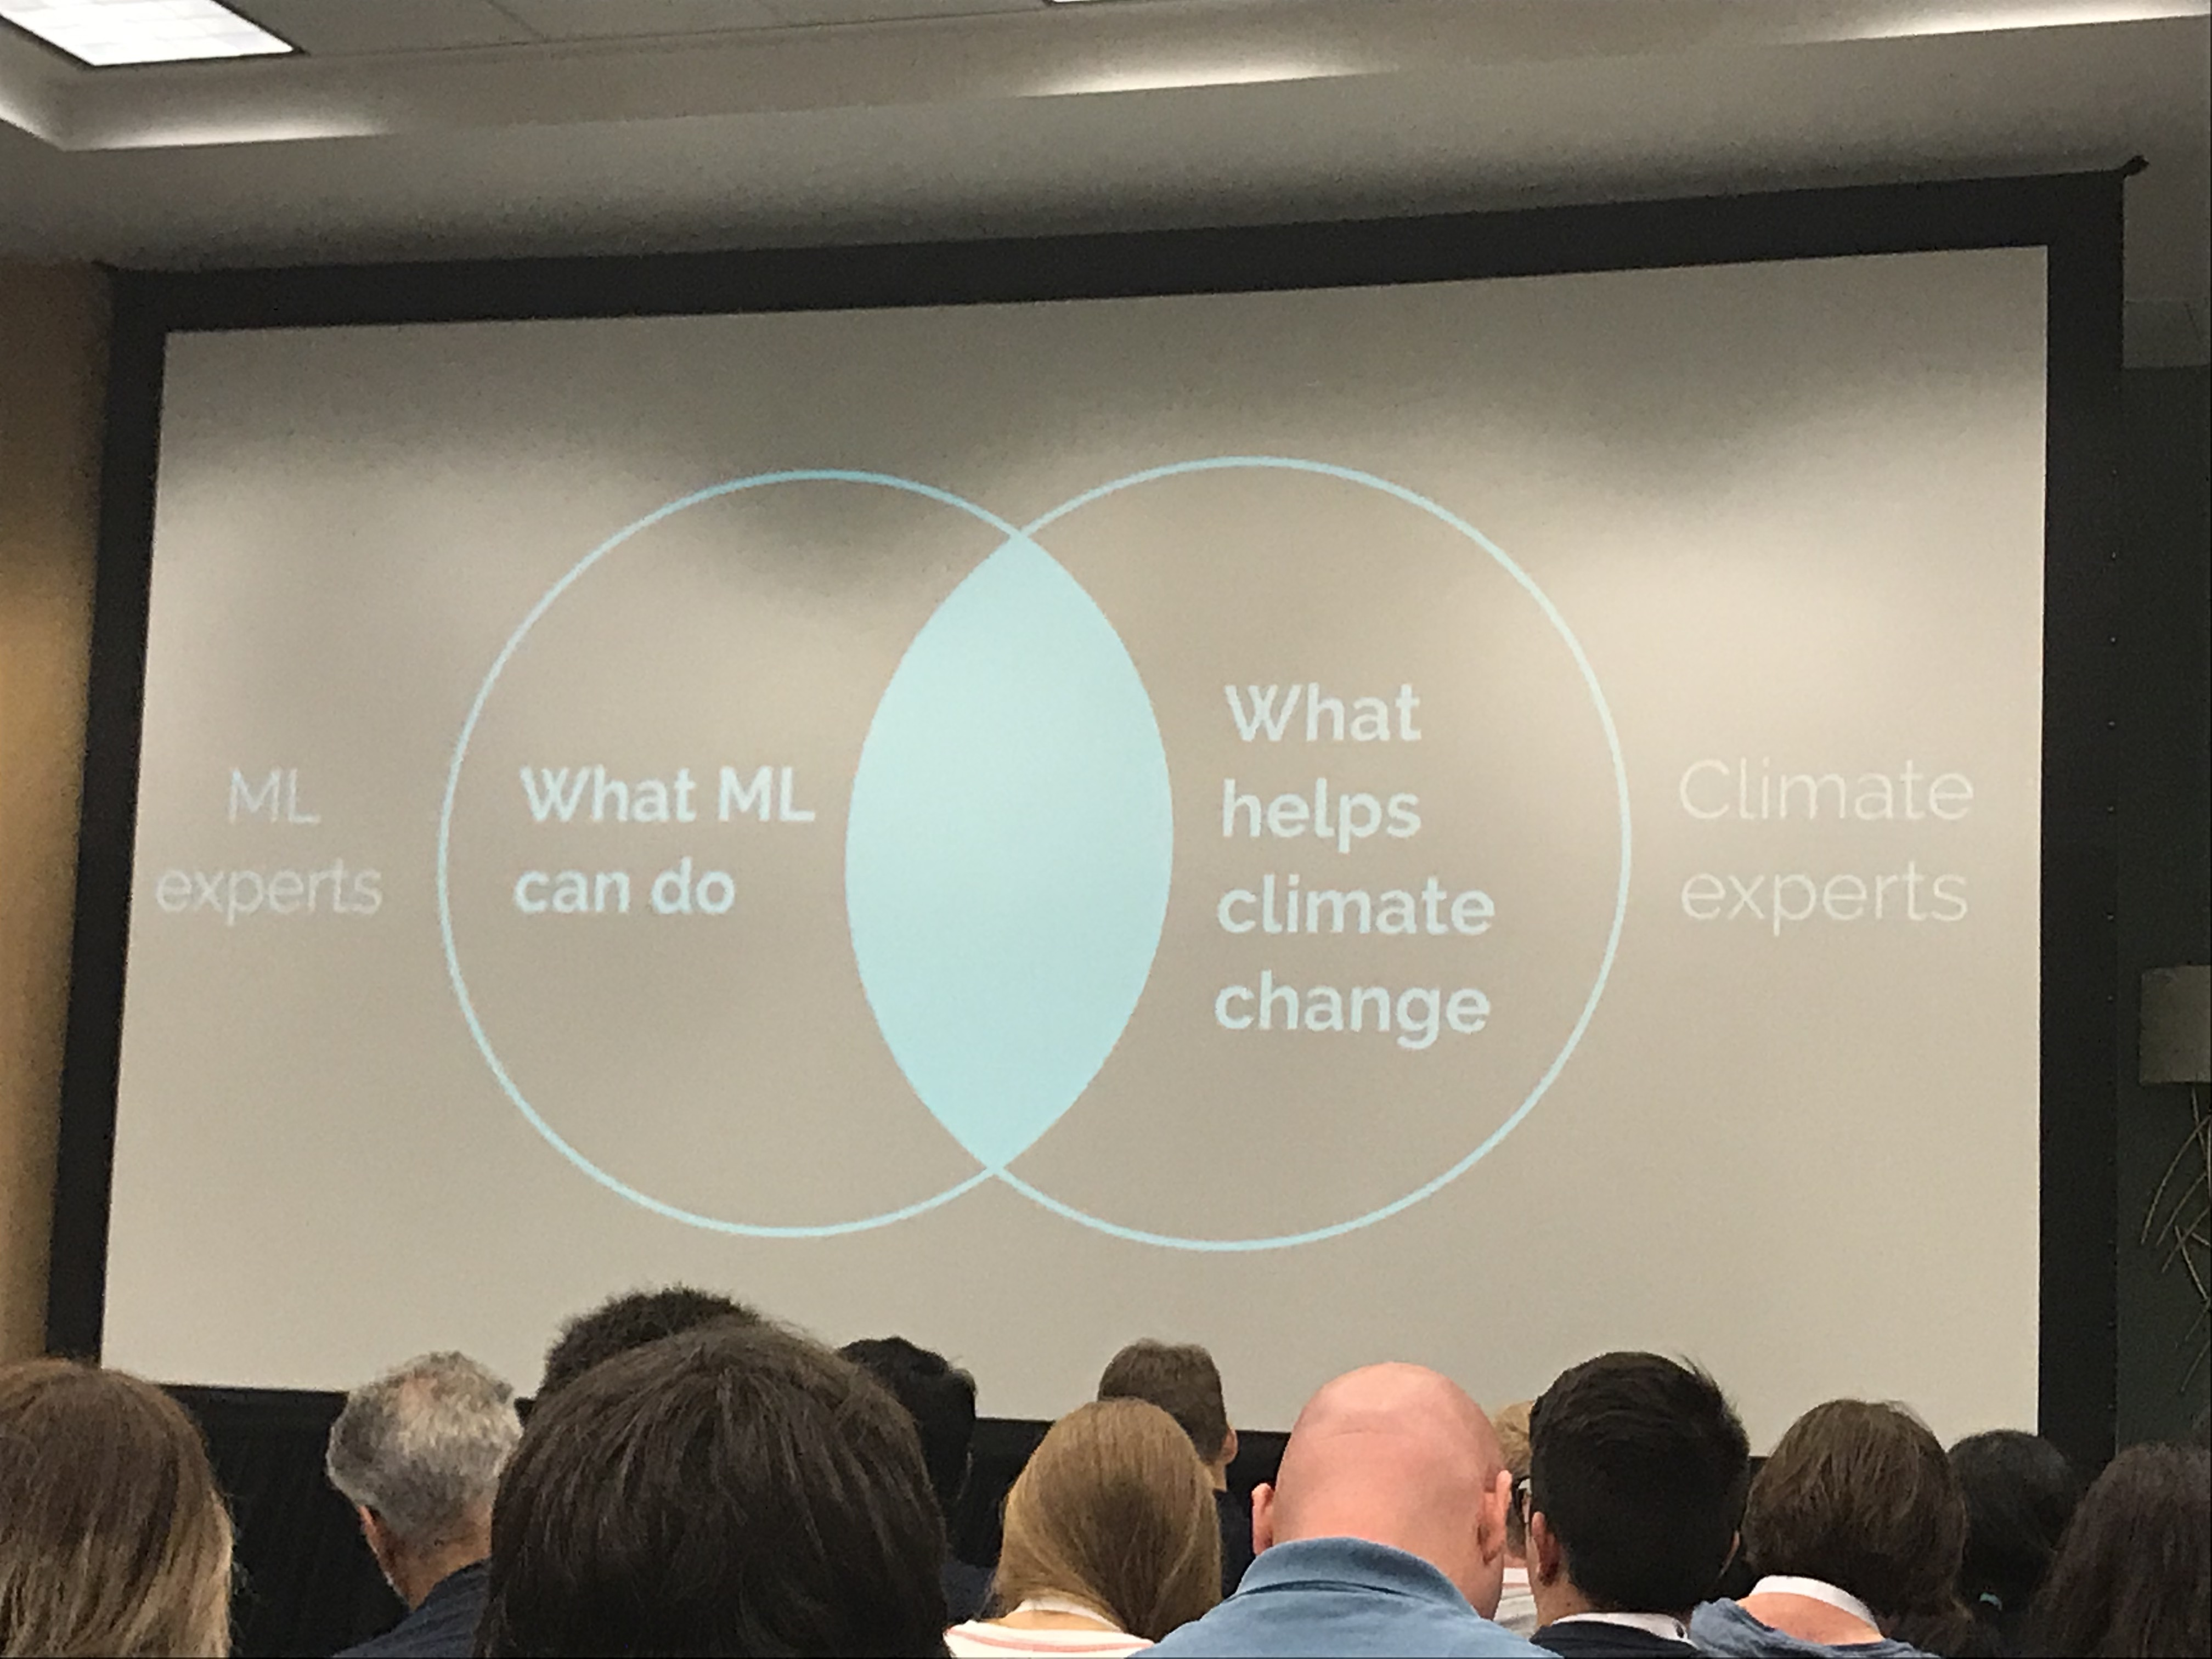
\includegraphics[width=0.5\textwidth]{images/venn.JPG}
    \caption{Call for collaboration across ML and climate science.}
    \label{fig:venn}
\end{figure}


{\bf Concluding thought}: In eras of technological disruption, collaboration matters. Work together! Share data! This problem is bigger than ourselves.

\spacerule

\subsection{Workshop: RL for Real Life}

I arrived just in time for the panel.

\subsubsection{Panel Discussion}
\label{sec:panel}

The panelists are Craig Boutilier (CB), Emma Brunskill (EB), Chelsea Finn (CF), Mohammad Ghavamzadeh (MG), John Langford (JL), David Silver (DS), and Peter Stone (PS). I'll abbreviate each by their initials. \\

Moderated by Alborz Geramifard (AG). \\

Q: What application areas are most promising for RL and why? \\

JL: Bread and butter baseline is personalization---of news stories, of advice, layouts, many other things. \\

CB: For me, interested in agents that can act on behalf of users, lots of problems though (multi-agent, preference elicitation). Recommender systems are promising but also challenging. We won't see wins short term, but recommender systems long term over long periods of time should serve as a really valuable test bed and a way to stress RL algorithms. \\

PS: We need a definition of promising to answer the question. Excited about promise of RL in robotics and manipulation, like my colleagues, the general class of user engagement through nudges/influencing people's behaviors in helpful ways (insidious ways, too, though). Help people rehab or take medicine; well fit for RL. We do have to think about what settings in the real world are safe/well fit. \\

CF: The best fits for RL are not really the problem the community focuses on. MuJoCo for instance has served its purpose for a time, but we need to scale now to partial observability, transfer, continuous state/action. Robotics fits that well though. \\

JL: Moving beyond bread and butter that are deployed right now, I think system optimization is a natural area for RL application. Most of these systems have a good recording over time, so lots of data (and don't have to wrestle with uncertainty). \\

EB: Personalization is a raw term, lots of things are changing in the world. Prior applications (when I was in grad school) was robotics and games. Opportunities now for personalization, given the world right now, is both a huge responsibility {\it and} exciting opportunity. \\

DS: Follow up to something John said in his talk---if we get the foundations right, there will be applications everywhere. If we get an algorithm that just works, we should expect to see RL in all kinds of places. Who knows what methods/approaches are out there? Let's continue to push the foundations. We should of course keep pushing and try to deploy it too, but I think we can expect to be surprised too. Looking a little farther in the future, one open area where there's huge potential for getting RL right is personalized health care. Can transform many people's lives. \\

MG: Lots of OR applications everywhere---think about system optimization, huge opportunity for RL. What's happening with Amazon storage facilities. One more thing for recommendation systems. Recommender systems are everywhere and we have tons of data. Consequences of our actions are clear, need to consider safety and robustness. Although consequences of actions in recommender systems aren't catastrophic, it's still important we get it right. \\

\spacerule

AG Q: Great segue into next question. How should we explore in these problems? \\

DS: Part of every framework, even in simulation. We always have to handle explorations (agents die, we don't receive more reward/data). If it has opportunity to come back and learn more, then we can still learn from the {\it lack of experience} to get more. That's nice in recommender systems too since we get ``parallel lifetimes", if a stream of experience stops we can still learn from it. It's signal that someone stopped using the system \\

CB: Yeah except for people that die in certain trajectories. Maybe not in recommender systems but in broad multi-user systems. In multi-user systems you get to distribute these decisions/explore. Can learn from individual users in a distributed way to guarantee safety (no individual action that can be so bad). In clinical setting, in recommender setting, can distribute exploration to not do damage to any individual. \\

EB: I think this is a really interesting question in a lot of settings---it's a reason to use policy gradients or imitation learning or methods with monotonic improvement. Some work shows we can be optimal too (be greedy w.r.t. information we have so far can still do well). These kinds of approaches help us avoid the major burdens of exploration. Lots of tools and directions to make progress. \\

PS: To me it's a fascinating question of meta-learning. When we do have a big population of users, should we pick a small subset and burn them and use our exploration budget, or should we explore a bit across all users (or other strategies)? Meta-objective: keep population happy with what you're doing, so: how should we achieve this? \\

CB: Quick response. If we have a model of cost of exploration this all falls out of the wash.\\

JL: This is a place where theory is really important. If we're going to optimize only for efficiency, you'll be driven away from $\eps$-greedy, and if we want to think about safety, we can use bounds to guide decision making in a safe way. \\

MG: Ways to make exploration more conservative. How conservative can we be? Well that depends on individual task/product/setting. If we know information about users/domain, we can set the exploration appropriately. Another important question: how do we fill the gap between simulation and the real world? Really hard. But having those simulators will help us explore in the world. \\

DS: Even in the real world, there are times when users leave, and we can actually continue to learn from these settings. If we do it right, it's all there in the framework: how should we maximize reward? Sometimes we take actions that keep people engaged or not, and that's ok. \\

EB: One thing we've been thinking about is how to keep exploration safe. Idea: policy certificates. Can promise explicitly how a particular method will explore/behave. We can have tools that can allow us to expose when we're going to explore and when we won't.

\spacerule

AG-Q: What are general principles that are key for bringing RL to the real world? \\

JL: First principle is that the framing of the problem is more important than anything else. Second one: if I gave you a long laundry list of things that are more important in real world than simulated worlds. \\

CF: One principle important to safety is to {\it identify} cases where it's safe to explore. Maybe you buy a small robot first and then transfer what it learns (like it's okay to fall down as a kid to learn from it). Identify situations where it's safe to explore, then can maybe be equipped to explore in new situations. \\

PS: Biggest lesson---simulators are never perfect! Super appealing because they're safe and we can get lots of data. We should use simulators, but we're never going to get them perfect. Efforts to make simulators perfect are misguided we should make new methods. \\

CF: Completely agreed! If you could make a simulator that's perfect you've already solved the problem. Learning in the real world is going to be required. \\

CB: One other principle I'd like to raise---reward function and objective function design. That first reward function you specify is never the right one! We walk away and say ``this is the best policy", but it's clearly not based on the behavior, we got the reward function wrong. Human-in-the loop methods are really important for correcting/designing the right objectives/reward functions. \\

EB: I want to echo that---my lab does a lot of work in education and health care. Coupling this work (and these choices of reward functions) with domain experts is massively important. The first known application of RL to education was in 1999 to understand how students do well on problems. Example: give students problems until student gets it right, then give the student the same one over and over again (exploit!). \\

DS: Number one principle in my own work---scalability. We should only try to strive for methods that scale well with resources (three: 1) compute, 2) experience, 3) memory). If we can achieve that level of scalability, we just need to scale up the resources. If we design something where we put a ceiling into the method itself (stop exploring, stop learning, other constraints), that ceiling will hurt us. Goal should always be scalability.  If you look at the success of deep learning, I claim it's successful because it scales with all three things (compute, experience, memory). It does better and better with these resources. So we should find the RL methods that scale. \\

MG: First principle is to make sure RL is the right solution for your problem. Second, make sure we have the data available for RL. Think about supervised learned, if half your data is bad, you can still do well. Same situation for RL we can't do well. Reiterate what Craig said: reward functions are super important. Part of the reward function might be company profit (as opposed to say, customer happiness). \\

JL: I want to mention I agree with David. The process of educating people on the realities of RL is always fun. \\

PS: The design principle of our platform at Cogitai is a two part hypothesis: 1) RL is ready for the real world (that is, we, in this room, are ready to solve problems in the real world), and 2) the real world is ready for RL. This second piece is what John mentioned. Lots of problems in the world we know RL is ready, but it's a big challenge for us to work with folks from outside RL/ML to help them identify which problems are RL problems and help them use RL tools to solve their problems. The first bucket is easy (us find RL problems) while the second is hard (convince others). Important point from David: we're going to be surprised! It wasn't the people that made the smart-phone that built the apps. We build the technology and tools that enable people outside this room to use these ideas. That's the goal. Get it robust enough that we can be surprised. \\

CB: Widespread acceptance of RL is ultimately an important goal. We could have been having this same conversation $N$ years ago about ML in industry. Not very long ago just getting ML to be accepted in large scale production systems, but here we are. \\

\spacerule 

Audience-Q: (paraphrased by PS): can we compare approaches to supervised learning and RL on real problems? \\

PS: Well, I don't think it's well posed to do this test. There are RL problems and supervised problems. These are different. \\

JL: Consider recommendation. Enormous number of actions. To apply RL to an enormous number of things often won't work. If you have a supervised signal source, that doesn't suffer from same sample complexity issue. Could apply RL on top to get the personalization which you can't really get from SL. There is no representational limit to RL---the same representations that can work for SL can work for RL. We've done reductions between these and this works. \\

CB: You can treat RL problems as supervised learning problems in recommender systems. Make a prediction, store it. The differences is whether we're being myopic vs. looking at the long term. The question is, if you learn representations about how users act in long term vs. short term, do you get some benefit? I don't know. \\

DS: A comment about A-B testing. You raised it as if it were outside RL, but you can think about it as a bad RL algorithm. Do this one thing and stick to it, do this other thing, then compare how these do after the trial. That's part of RL but we can also do better like contextual bandits. \\

\spacerule

Audience-Q: On horizons/reward design. Algorithms might exploit human weaknesses more heavily in the future, a lot of the behaviors of ML algorithms are probably due to their myopic nature. Being able to look ahead for multiple time steps might allow for better reward functions. Thoughts? Second, when we use RL for problems with humans in the loop, what is the longest horizon we can actually use. \\

JL: Right now, typically, horizon is relatively short (hours, minutes, days). As that increases data is harder to come by. If we succeed in RL there's no reason it can't be lifetimes. \\

EB: Depends on what level of granularity you're using: hierarchical can help here! Both of those views are definitely possible. The technology we're developing is dual use and an amplifier. Will be constrained by the people and not the techniques themselves. \\

CB: Totally agree with with John and Emma. I still don't think we have the technology in our hands to do multi-scale planning, but we'll get there. With respect to doing right by the user. One important thing: we really don't have good methods for understanding user preferences and utilities, and how their behaviours reveal these. Real limiting factor to applying RL over long horizons is a developing techniques where we can know quickly what a users' utility function is. RL is also about planning but we're far from being able to do that.

CF: On reward design and David's comment about scalability---we should be thinking about algorithms that scale, but if we're in the real world, reward function supervision isn't a scalable source of feedback. In those settings is important to consider how we should frame the problem so it's scalable. Shouldn't be afraid to change the problem statement. For example, if you want a scalable algorithm, design a setting and algorithm that can scale with the resources involved. Don't really feel constrained by the classical RL statement if your problem doesn't match that.

\spacerule

Audience-Q: First, when is a policy safe to deploy? \\

PS: Tempting but wrong: Deploy when optimal! Will definitely depend on domain. Testing should be empirical---can we drive better than people? \\

EB: Can learn a lot by looking at verification (in RL, in deep learning). For these examples, sometimes people can't be in the loop to verify. Can use these to avoid worst-case scenarios (see: making aircrafts avoid collisions). Some safety guarantees. \\

JL: Practical answer: frame your problem so no actions are particularly bad/catastrophic. Then do RL on top of that.




PS: RL has components that are Art and components that are Science. We've been trying to make it 100\% science, but we need to accept that parts of it are art.

\spacerule


{\it Lihong Li on closing remarks:} 
\begin{itemize}
    \item Goal of workshop: Bring together researchers and practitioners from industry and academia interested in addressing practical and/or theoretical issues in applying RL to real life scenarios. 
    \item RL in real life: games, robotics, transportation, resource allocation.
    \item Challenges: partial observability, multi-agent systems, stochasticity, large action set, simulators, evaluation, generalization.
    \item Post workshop discussion via slack (on the workshop website: \url{https://sites.google.com/view/RL4RealLife}).
\end{itemize}


\spacerule

Next up is the afternoon session of a closely related workshop.

\subsection{Workshop: Real World Sequential Decision Making}
\label{sec:off_pol}

The workshop begins with an invited talk by Emma Brunskill.

\subsubsection{Emma Brunskill on Efficient RL When Data is Costly}

{\bf Questions:} What's the best way to teach a student coding? How should this patient be treated for cancer? Will job training increase future income? \\

$\ra$ We'd like to answer these question in an evidence based way! See: interventional science. \\

{\bf Problem:} The way we do interventional science at the moment is flawed. Example: run a bootcamp. See which intervention leads to higher graduation rates. One idea: dynamically adapt how we assign students to conditions. $\implies$ use RL! \\

$\ra$ Can use RL to understand the science of intervention. \\

Historical test beds: video games and robots. Now, though: new kinds of test beds. \\

Recent changes: massive compute, massive sensors, and ability to dynamically interact with people. 

$\therefore$ opportunities to apply RL have emerged! Lots of negatives to this, but many opportunities too. \\

{\bf Goal:} Learn to make good decisions faster (in a statistically efficient way), to benefit more people. \\

Q: How can we create AI that help students? \\

A: Project---RL assistance leads to 1.3$\times$ faster learning, longer learning, and more learning. \\

Key Techniques:
\begin{enumerate}
    \item Exploration!
    \item Counterfactual/Batch Off Policy RL (focus today).
    
    $\ra$ Tension between beautiful math and impacting society. But! This area allows for both.
    
    $\ra$ Growing interest in Causal Inference and ML. See: {\it The Book of Why} by~\citet{pearl2018book}.
\end{enumerate}

Q: How can we learn from historical sequential data? \\

A: It's really hard! Many challenges: data generation process is fundamentally different. That is:
\[
\tx{Different Policies} \implies \tx{Different Actions} \implies \tx{Different States}
\]
That is: decisions {\it compound}. \\

$\ra$ Moreover: we don't even know the behavioral policy. \\

{\bf Classic challenge:} Batch Off Policy Evaluation. We're given a dataset $D$ of trajectories gathered by some policy $\pi_D$, and we would like to compute the value of some new policy $\pi'$. \\

$\ra$ One spin: batch off policy {\it optimization}. Just want to know how to {\it act}, given data from prior policy. \\

Example: when should we treat patients? Really, how can we come up with a {\it personalized} policy for when to intervene (take a ventilator off, for instance). \\

$\ra$ One specific kind of intervention policy: vast majority of decisions are ``nothing", then suddenly we have to intervene. Let's call such a decision the \texttt{when-to-treat-policy}. \\

Q: When should we start HIV treatment? When should we stop some kind of treatment? \\

$\ra$ These cases are well captured by parameterized policies conditioned on relevant contexts. \\

Two solutions: Importance weighting (also called ``inverse propensity weighting"). Goal is to estimate expected value of new \texttt{when-to-treat-policy}. \\

$\ra$ Advantage: simple and consistent
$\ra$ But: uses only trajectories that match data, not very robust, high variance. \\

{\bf New Idea:} Advantage decomposition: $\tau_\pi$ is a stopping time w.r.t. some filtration \texttt{when-to-start-treatment} according to policy $\pi$. Then:
\begin{align}
\mu_{now}(S_{1:t}) &= \bE\left[\tx{Return}\right] \\
\mu_{next}(S_{1:t}) &= \bE\left[\tx{Return}\right]
\end{align}
If we can determine which $\Delta_\pi := V^\pi - V^{\pi_0}$, where $\pi_0$ is the \texttt{never-treat} policy, we can determine the advantage of a particular treatment. \\

$\ra$ Specifically: want to estimate $\Delta_\pi$ from data, even {\it without} $\pi$. \\

Yields the {\bf Advantage Double Robust} (ADR) Estimator for off policy evaluation in the when to treat context. Yields regret bounds, too. Further differences visualized in Figure~\ref{fig:off_policy}.

\begin{figure}
    \centering
    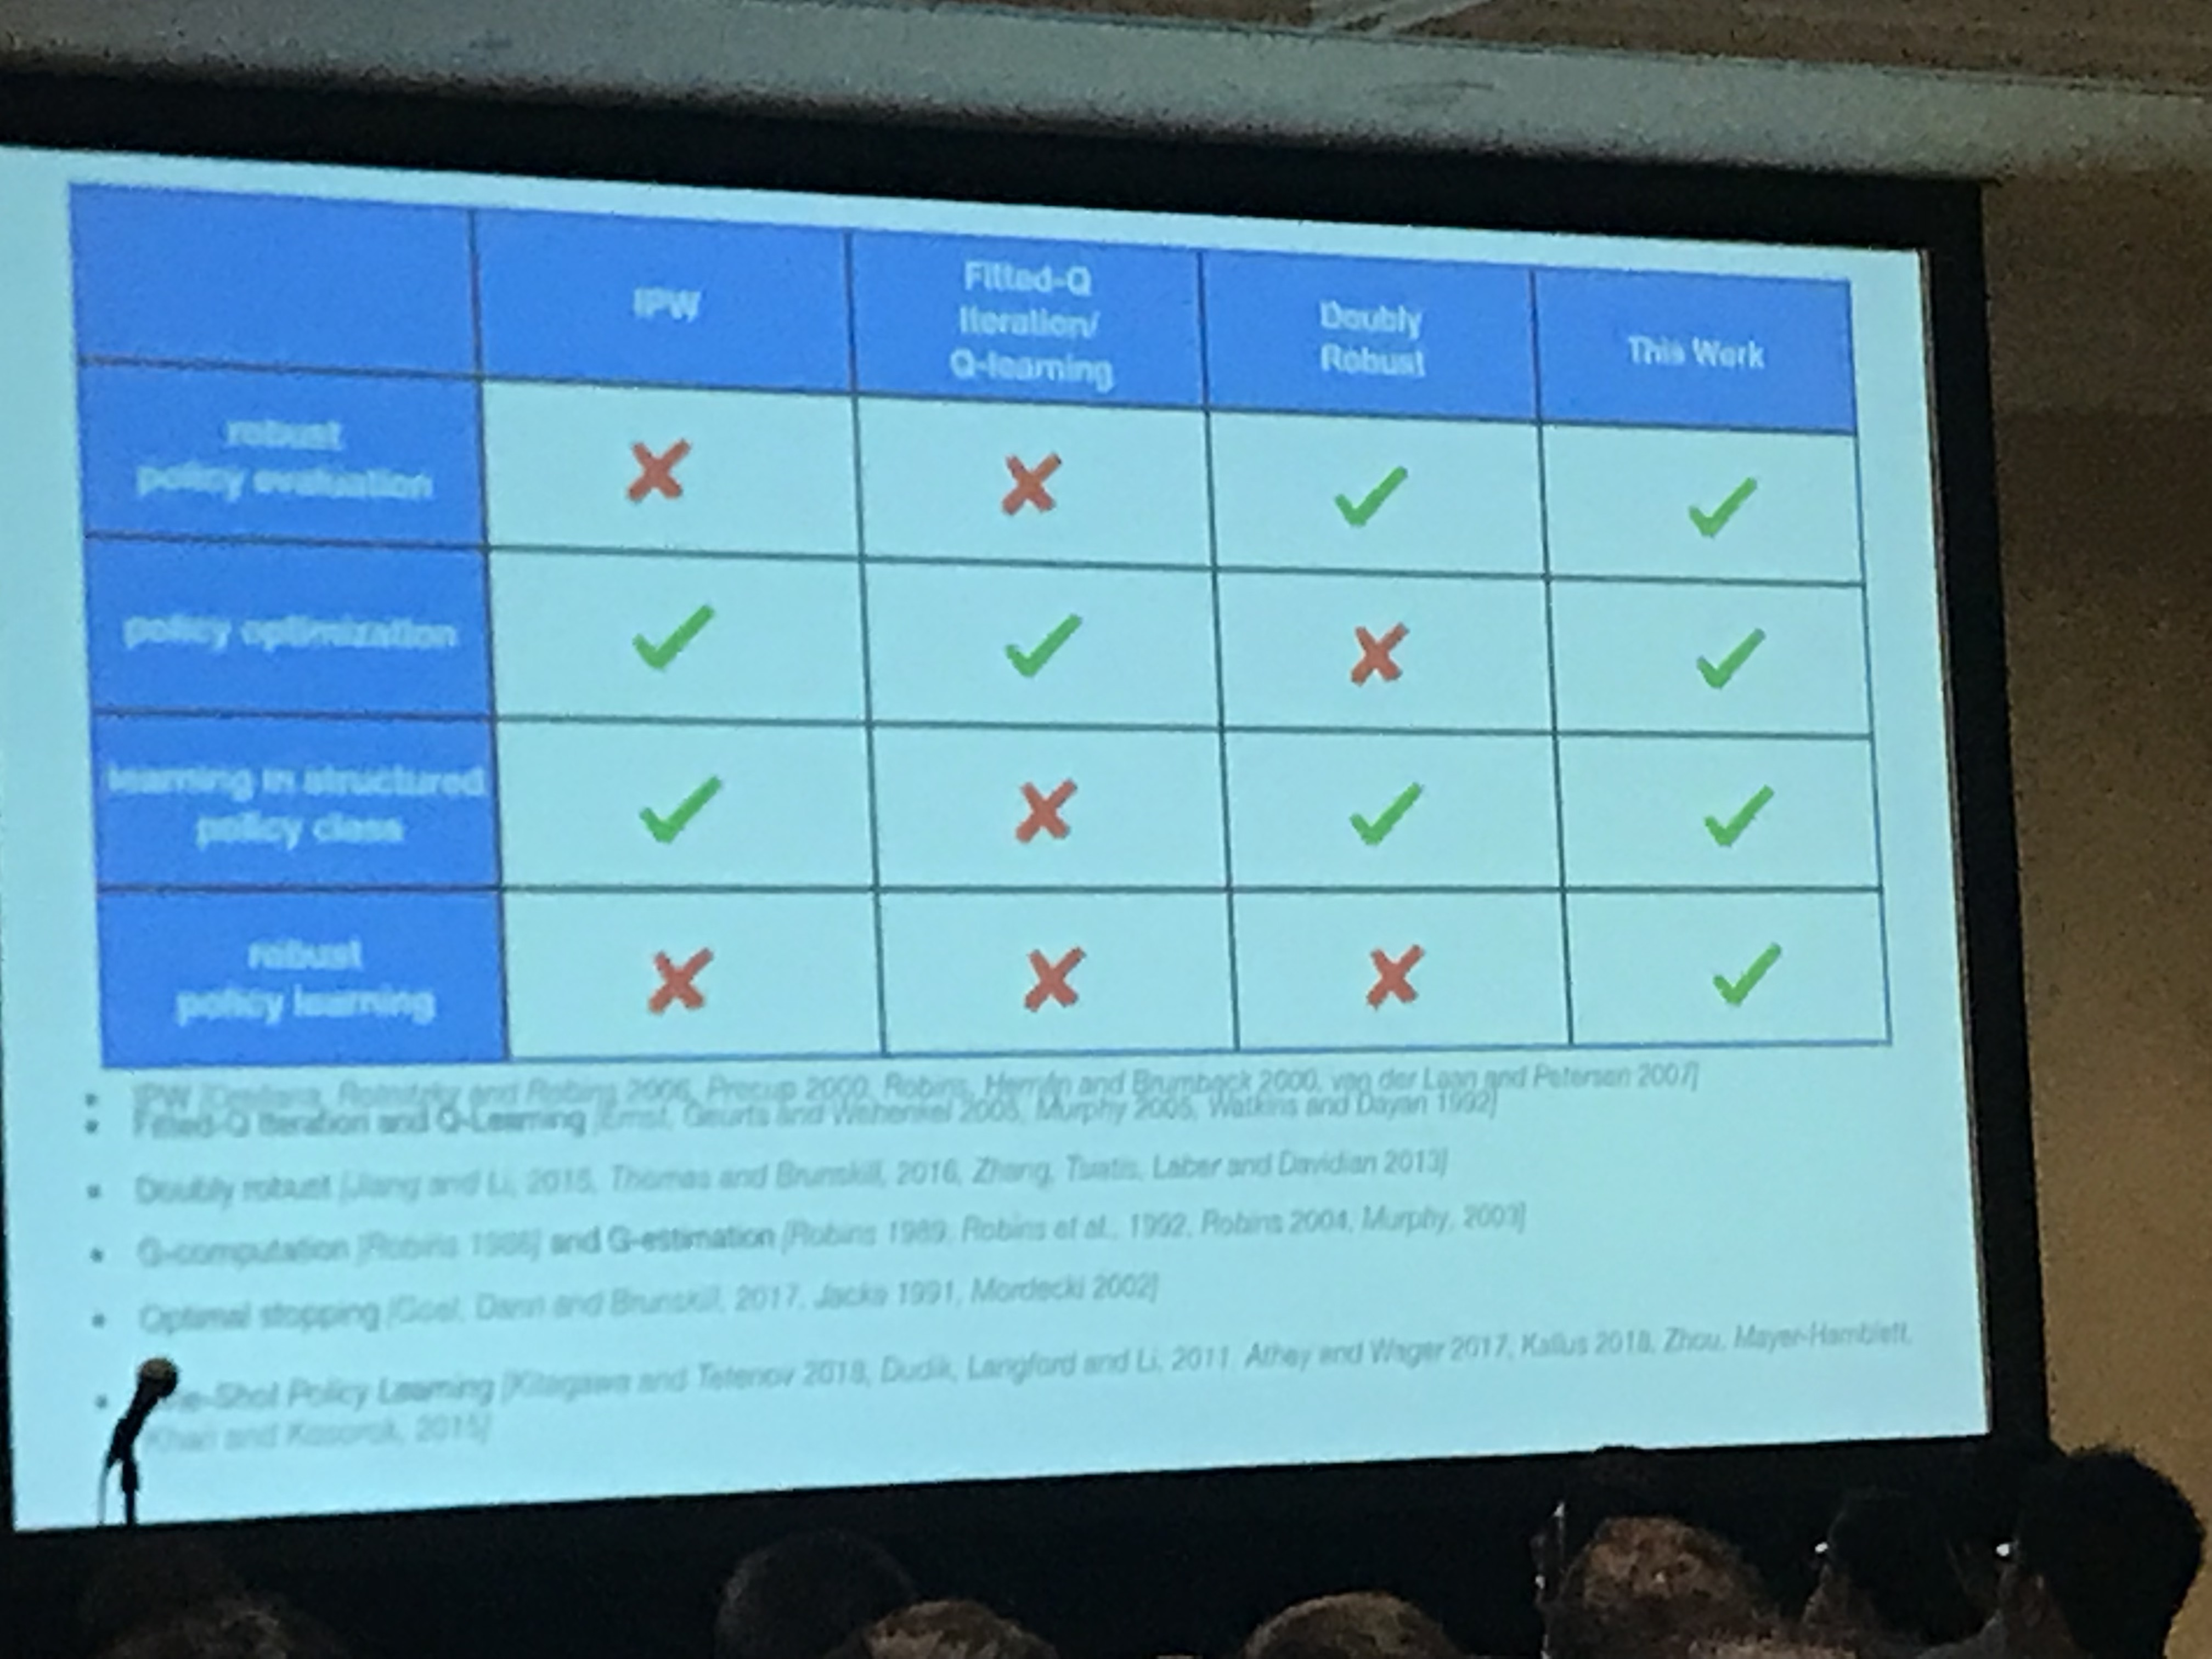
\includegraphics[width=0.5\textwidth]{images/off_pol.JPG}
    \caption{Comparison of different off-policy evaluation types.}
    \label{fig:off_policy}
\end{figure}

{\bf Experiments:} Keeping a health metric above 0, where state evolves over time in a stochastic way (with brownian motion). Use treatments to try to help outcomes. \\

$\ra$ Given observational data from clinic, want to find way to choose effective treatments. \\

Another important question: how can we estimate $V^*$? (perhaps, specifically to help human-in-the-loop)\\

Q: Can we identify with $< O (d)$ samples if there exists a linear threshold policy with expected value over a threshold $b$. \\

A: For some distributions over contexts, yes! This is before we could return any policy.

\spacerule


\subsubsection{Miro Dudik: Doubly Robust Off-Policy Evaluation via Shrinkage}

{\bf Problem Setting:} Contextual bandits. Comes up when learning from interaction data.\\

\ddef{Contextual Bandit}{An interaction protocol where a user comes to a service, the service presents objects to the user, and the user makes some decision based on the objects given. 

That is, we follow: 1) Observe context $x$, 2) Choose action $a$, and 3) Receive reward $r$, then sample a new context i.i.d.}

$\ra$ Lots of applications of contextual bandits. \\

Running Example: Think about news recommendation as a canonical instance of a contextual bandit. Repeatedly the algorithm perceives a context (user data), suggests some article to the user, and observes some data indicating the quality of the suggested article (click). \\

$\ra$ Challenging because reward model typically trained on prior data, $(x_1, a_1, r_1), \ldots, (x_n, a_n, r_n)$ (often for different policy). Moreover, policy by be randomized.

{\bf Fundamental task:} off-policy evaluation. What would have been the click rate if we had followed some other policy?

Standard Approach: importance weighted estimates. Reweight prior experiences according to:
\[
\frac{\pi_{new}(a_i \mid x_i)}{\pi_{old}(a_i \mid x_i)}.
\]

$\ra$ Unbiased, but high variance. \\

{\bf Key Question:} Can we take advantage of the reward estimator $\hat{R}$ to improve over these methods? \\

Two tricks:
\begin{enumerate}
    \item Doubly robust estimate: use direct estimate as a baseline, apply importance weighting to estimate the {\it departure from the baseline}.
    
    $\ra$ Still unbiased!
    
    \item Weight shrinkage (see justification below). Idea is to clip estimator with a parameter $\lambda$:
    \[
    \hat{w}(x,a) = \begin{cases}
    w(x,a)& tx{if} w(x,a) < \lambda\\
    \lambda& \tx{if} w(x,a) \geq \lambda
    \end{cases}
    \]
    
    Allows for $\lambda$ to control, explicitly, the bias-variance trade-off, while ensuring weights are smaller.
\end{enumerate}

\ddef{Doubly Robust Estimate}{The doubly robust estimator is as follows:
\[
\hat{V}_{direct} + \frac{1}{n} w(x,a) (r - \hat{r}(x,a)) ^2.
\]}

Critically: doubly robust estimator is asymptotically optimal, but in finite samples, other estimators tend to be more accurate. \\

$\ra$ Critically:
\[
\text{Mean Squared Error = Bias$^2$ + Variance.}
\]
But: IPS and DR are unbiased, so error is entirely variance. Their variances are:
\begin{align}
    &IPS: \frac{1}{n}\bE[w^2(x,a)r^2] + O(1/n) \\
    &DR: \frac{1}{n}\bE[w^2(x,a)(r - \hat{r}(x,a))^2] + O(1/n) \\
\end{align}

Even if $\hat{r}(x,a) = \bE[r \mid x,a]$, so $\hat{V}_{\tx{direct}}$ is unbiased, we suffer to due large weights if rewards are inherently noisy. Thus: weight shrinkage (see above). \\

Q: Many ways to shrink weights? Which one should I use? \\

A1: Pessimistic shrinkage! Only assume
\[
|r - \hat{r}(x,a)| \leq 1
\]
This induces bias of $\bE[(\hat{w}(x,a) - w(x,a))(r-\hat{r}(x,a))]$. \\

New variance $\leq \bE[\hat{w}(x,a)]$. \\

$\therefore$ Can come up with the right kind of weight shrinkage method. \\

A2: Optimistic shrinkage! Assume $\hat{r}$ is fitted by optimizing weighted square error with a weighting function $z(x,a)$:
\[
\frac{1}{n} \nsum z(x_i, a_i) (r_i - \hat{r}(x,a))^2
\]
Then we can bound the bias and the variance again (using similar pareto-optimizing-trick). New estimator based on $\lambda$:
\[
\hat{w}(x,a) = \frac{\lambda}{w^2(x,a) + \lambda} w(x,a).
\]
As $\lambda \ra \infty$, leading coefficient becomes 1, recover DR estimator, as $\lambda \ra 0$, recover the \dnote{Missed it.} \\

{\bf Experiment 1:} Do we need both optimistic and pessimistic shrinkage? How often across 108 conditions is each better? (for three different choices of reward predictors). \\

$\ra$ Finding: under all three reward predictors, pessimistic shrinkage tends to be better than optimistic is better (but there are conditions when optimistic is better, or they tie).

{\bf Experiment 2:} Do we need all these reward predictors? \\

$\ra$ Finding: Again, some cases where each predictor is superior (when using the direct estimator).
$\ra$ When using DR almost always a tie across the different estimators.
$\ra$ Moreover, when using DR with shrinkage, one of the reward estimators $(z=w^2)$ suddenly becomes dominant. So: if using shrinkage, might need to rethink how you're using reward estimators. \\

{\bf Summary:}
\begin{itemize}
    \item For best finite-sample performance of DR:
    $\ra$ Important to consider both reward predictor and weight shrinkage
    $\ra$ Different reward predictors applicable in different settings
    $\ra$ Model selection matters and needs to be studied more
    \item Next steps: structured actions, continuous actions.
\end{itemize}


\spacerule


\dnote{And that's a wrap! Sadly I have to miss the workshops tomorrow (and the rest of today's session). Flying out of Long Beach shortly.}



\section*{Edits}

Many thanks to the following individuals for sending along helpful edits/catching typos:
\begin{itemize}
    \item Zeno Zantner for catching typos.
    \item Brandon Amos for catching typos.
\end{itemize}


% --- Bibliography ---
\newpage
\bibliographystyle{plainnat}
\bibliography{icml}

\end{document}